\documentclass[lang=cn,10pt]{elegantbook}
\usepackage{physics}
\title{Mathematics in Quantum Chemistry}

\author{J.M.Anderson (美)}
\bioinfo{翻译}{邹宪法}

\extrainfo{Too young too simple, sometimes naive.}

\setcounter{tocdepth}{3}

\cover{cover.jpg}

% 本文档命令
\usepackage{array}
\newcommand{\ccr}[1]{\makecell{{\color{#1}\rule{1cm}{1cm}}}}

% 修改标题页的橙色带
% \definecolor{customcolor}{RGB}{32,178,170}
% \colorlet{coverlinecolor}{customcolor}

\begin{document}

\maketitle
\frontmatter


\mainmatter

\chapter*{译 \ 者 \ 的 \ 话}
\setcounter{page}{1}
\pagenumbering{roman}
偶读此书,顺便译出。
作者在这本书中只介绍了两个数学课题——正交函数微积分,向量空间代数和两个物理课题——拉格朗日经典力学,哈密顿经典力学。
其取材精炼,针对性强,对初学量子化学的同志,是一本值得参考的书。
故将其初稿重新整理出版,并对原书中某些文字上的错误做了修正,对原书所附各章习题答案并未做核对,仅供参考。许多同志对初稿提出了不少宝贵的意见,在此一并致谢。
限于译者水平,译文有不当之处,希望读者指正。
\begin{flushright}
    译 \qquad 者 \\ 一九七九年十月
\end{flushright}
\chapter*{来自\textit{Astolfo}}
在图书馆中偶然碰到此书,不忍心让如此良物沉寂在图书馆的地下室中,且寻不到PDF版,遂决定将其誊写一份。
在誊写过程中,本人的一些想法将在本书的脚注中陈述。感谢同学
\begin{Large}
\textbf{卷王}
\end{Large}
帮忙从图书馆借下此书并绘制图片(30\%的图片),本工作得以顺利进行。
限于本人水平,誊抄若有不当之处,希望读者指正。
\begin{flushright}
    \textit{Astolfo} \\ 2022年2月
\end{flushright}
\chapter*{序}
化学教育今年来的发展趋势,迫使学化学的学生在学习进程中接触量子力学的应用越来越早。
本科化学课程表的这一发展方向之所以重要其原因如下:
物理-化学信息的宝库来源于建立在量子力学的基础上的分子光谱和其他技术,表述化学的发展趋势是建立在量子力学提供的概念的基础上;
理论化学的发展方向是用量子力学充分解释分子现象。

将同学骤然引到这种艰难和令人激动的学习中,常使他们不能适应表达这些内容的数学公式,把握不住已经习以为常的牛顿世界和分子现象世界之间的联系,不能将新建立的理论知识应用到分子结构和分子运动问题上。

在本书中我们只准备讲数学中两个重要课题和物理学中两个重要课题。
它们是数学中的正交函数微积分和向量空间代数,物理学中的拉格朗日经典力学和哈密顿经典力学及它们在分子运动中的应用。
我选择这四个课题是因为它们与现代量子化学密切相关,特别与量子力学在分子光谱中应用密切相关。
对分子光谱的强调反映了我个人对这个成长着的和普及的领域的兴趣和工作;它也使我从这本小书中去掉了对我的同时和他们的学生感兴趣的课题。
我们去掉了小定理,电学,磁学和辐射物理,因为它们在别的书中一般讲比本书处理得更好,并且容许做更深入的讨论;由于同样原因,将群论与微分方程包括近似解法也留给别的书来讲。

本书试图一般地为量子化学,特别为分子光谱准备物理和化学基础。
读者应有包括偏微分和重积分在内的微积分(通常约为一年半),一年物理和一年化学的准备知识。
这个材料曾用做Bryn Mawr学院,为具有上述准备知识的同学开设的一学期课程“化学家用的应用数学”的基础;在此课程后接着学习初等量子力学。

作者对Addison Wesley出版公司允许从其出版物上取材和W. Z. Benjamin公司的不断帮助和鼓励表示感谢。
\begin{flushright}
    Jay \ Martin \ Anderson \\
    Bryn \ Mawr Pennsylrania \\
    1965年10月
\end{flushright}
\tableofcontents
\thispagestyle{empty}
\newpage
\setcounter{page}{1}
\pagenumbering{arabic}
\chapter{导言}
\section{量子力学中的本征值问题}
与量子化学有关的数学和物理,几乎没有例外,都是面向求解一类特殊问题,即用组成体系的粒子的基本性质(电荷,质量)计算分子体系的性质。
只用电子电荷,普朗克常数等计算分子中电子的能量就是一个很好的例子。
读者或已知道这个问题的答案的本性\footnote{个人感觉翻译成本质更好}了。
分子中的电子的能量可取一些分立值,但当能量的值高达某一点后再高的能量值则在连续区中。
这些能值定性地示于图1-1中。
正如实验指出的那样,量子力学为某些物理量提供的结果是它们只能取某些值而非全部值。
一物理量的许可值称为本征值,他来源于德语特征值。
一特殊物理量的本征值可取值于连续区或取自有限或无线的一组分立本征值中。
例如,一个原子的能量可以是无限多个分离本征值中的一个,也可以是更高区中的称为连续谱的本征值中的一个。
化学设计的物理量多半是分立本征值而非连续本征值\footnote{大概是由于基本在处理电子态处于基态时的分子。}。
\begin{figure}[htbp]
    \center
    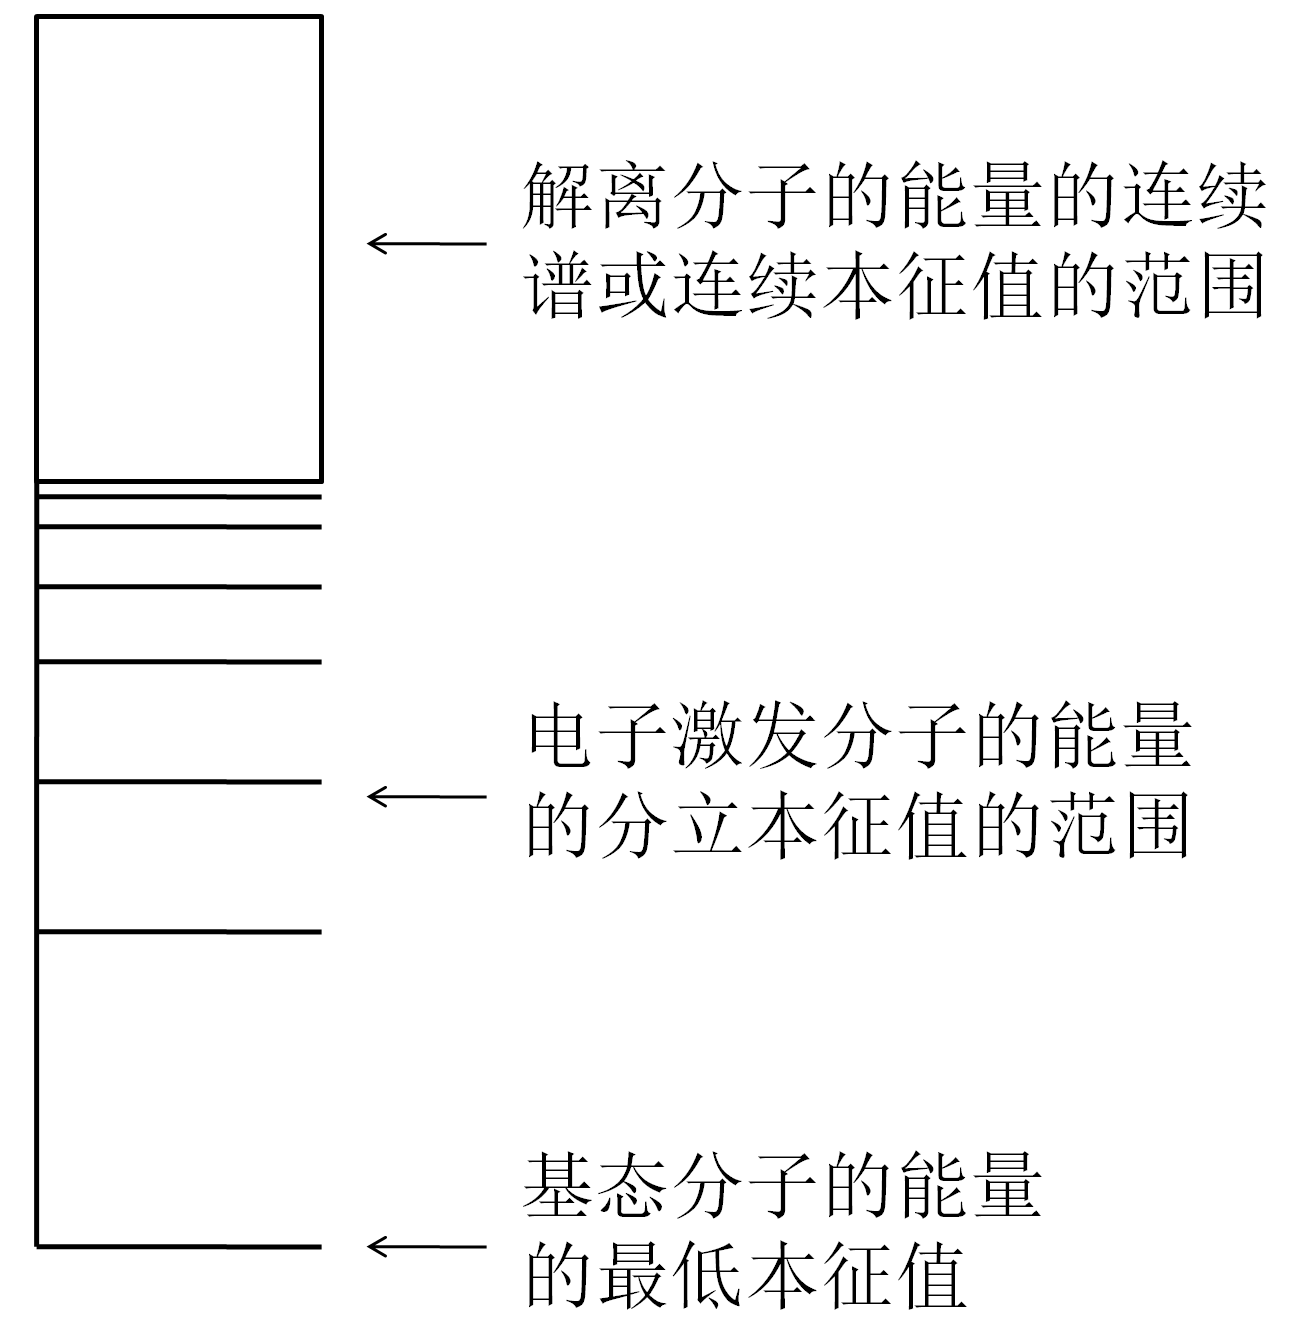
\includegraphics[scale=0.15]{./fig/1-1.png}
    \caption{分子的能量的本征值}
\end{figure}
求一物理量的本征值的数学问题称为本征值问题;用通常称为本征值方程的那种形式的方程计算。
一物理量Q的本征值方程具有易为人误解的简单外观:
\[\hat{Q}f=qf \tag{1-1}\]
方程中f是一函数,称为物理量Q具有本征值q的本征函数。符号$\hat{Q}$称为算符,$\hat{Q}f$这个陈述式告诉我们如何将函数f按$\hat{Q}$的定义中的含义所指出的那样换成一个新函数。
本征值方程(方程1-1)表示将算符$\hat{Q}$所示的那些规则用于f得到的函数是原来函数f的q倍。
很值得提出的一种情况是几根本征函数具有相同的本征值;即$\hat{Q}f_1=qf_1$,$\hat{Q}f_2=qf_2$等等。
在此情况下可称q是简并\footnote{原文中“简bing”的bing为“左伴随”单人旁的“并”,在LaTeX中打不出来,故用“并”代替}的,具有相同本征值的本征函数的数目叫做简并度。

算符可以只是数或函数;例如,可定义算符X为“对被运算函数乘以x”;因此$Xx^2=x^3$。
另一方面,算符可以比数或函数更复杂些。
例如,同学们已经使用过的下述算符(虽未用算符这个名称),它表示或定义为“求某变量的改变”。
例如$\Delta$作用于热力学函数H(焓)得到新函数$\Delta H$(焓的改变),$\Delta H=H_2-H_1$。
人们熟悉的另一算符是$\dv{x}$,他用于表示“对x求导数”。

如何写出对应于欲测物理量的算符是量子力学的任务。
目前我们的任务是学习如何求解这类算符的本征值方程,特别是学习用于讨论方程的解的性质的词汇和概念。
而量子力学本身是从两个不同的观点发展起来的,这两种观点代表本征值问题的两个类似的数学处理。

第一个观点是薛定谔的波动力学。
在波动力学里,算符是微分表达形式,像前边提到的算符$\dv{x}$那样,因而本征值方程区微分方程形式,可应用微积分学求解。
第二个表述是海森堡的矩阵力学,在矩阵力学中算符表示成叫做矩阵的代数形式;代替本征值方程中是函数,矩阵算符作用于向量$\zeta$将$\zeta$变换为与$\zeta$平行的向量,后者的长度是$\zeta$的q倍。
\[\hat{Q}\zeta=q\zeta \tag{1-2}\]
方程1-2是本征值问题的矩阵力学陈述形式。
在第三章中将对矩阵和向量给予定义并作详细讨论。
如方程1-1那样,q是物理量Q的本征值,$\zeta$是本征向量,$\hat{Q}$是用矩阵表述的算符。
这种形式的本征值问题的求解是用代数学。

量子力学的这些表面上不同的数学和物理处理方法,实际上有着深刻的相互联系;狄拉克的工作证明了两种观点的内在等价性,也证明了对应的数学技巧的内在等价性。

\section{经典力学的本征值问题}
我们已经简要地讨论了量子力学中本征值方程的作用。
但经典力学中的一些问题也可以用简单而有意义的方式表示为本征值问题。
其中力学体系(如分子)的振动和转动就是这类问题。
这些物理问题对研究分子运动和光谱学的化学家很重要。
在振动中,振动的简正方式和频率可表现为本征向量和本征值;在转动中,从本征值问题中可以得出主轴和惯性矩。
但应注意,在分子水平上正确地描述这些体系,总是需要量子力学,而非经典力学。

\section{本书涉及的范围}
根据我们希望能提出的,求解的和理解的问题的种类决定了的要求,在本课程中先学习与本征函数密切相关的一类函数,然后学习向量代数和矩阵代数,最后将本征值问题的两种观点综合起来。
并用经典力学的研究收尾,即了解如何将力学体系(如分子)的振动表示为本征值问题。同时试图将牛顿力学以它与量子力学的关系很清晰的形式表示出来\footnote{这里感觉作者翻译得有问题,我猜大概是想表达“同时试图将牛顿力学与量子力学之间的关系以很清晰的方式表达出来”}。

我将沿此途径学习本征值问题的一些方法,并采用一些化学中感兴趣的应用。
我们的着重点始终是概念第一,方法第二,而将数学定理的详细证明放在最次要的地位。
在每章后给出一组习题。
许多习题的答案和提示放在全书的后面。

\begin{problemset}
    \item 求算符$\dv{x}$的本征函数。
\end{problemset}
\chapter{正交函数}
对应于重要物理量的算符的本征函数,几乎没有例外,都有两个性质:正交性和归一性。
本章的目的是详细地展开这些概念和说明它们的一些应用。 
“展成正交函数”是最重要的概念。
做为这种技巧的举例我们将详细地考察“富里叶级数”。
我们也要学习怎祥用"施密特正交化”造正交函数和怎样从特殊微分方程的解产生正交函数。
为了说明后一概念, 我们将要考察“勒让德多项式”的性质,并简要介绍量子化学中其他重要特殊函数。
在附录中简要地讨论微积分和复变数的基础。
在学习本章前读者最好先检验一下自己对这些内容熟悉的程度。

\section{基本概念:正交性和归一性}
在开始讨论正交函数时,先复习函数概念。
函数概念有三个主要成份。第一,将函数定义在数标上的特殊域内,如从a到b。
第二,存在一变量(如x),它可在a到b域内独立地取值,第三,按特定规则对任意x值都存在确定y值。\footnote{换成我们现在比较熟悉的说法:构造函数这一映射关系需要一个定义完备的定义域和值域以及一个从定义域到值域的映射关系。}
这样,我们可以说在$a \leq x \leq b$域内y是x的函数。
这个定义可用某种方式加以修改以包含多于一个独立变量,但这三个主要成份要保持:一个独立变量;独立变量取值的区间;用一特定规则将因变量与独立变量联系起来。

表述“y是x的函数”的最简单的表示方法是写下方程y=y(x)。
这种表示法很简洁,但可能产生误会。
方程的左端仅是变量的名称——在我们看到方程右端之前并不知它是因变量。
右端也用字母,但这里的符号y( )的含义与单纯变量名称有所不同。
y( )表示y是因变量,它的值可按特定规则由括号里的量求出。
y=y(x)没表示出独立变量x定义的区间。
这在函数概念的初级讨论中并不总是重要的,但在表示函数展开时则是非常重要的。

因此,我们引入一个定义。
\begin{definition}[展开区间或简称区间]
    展开区间是所讨论的函数的独立变量的取值范围。这并不意味着在独立变量取其它值时函数不能定义,只不过不考虑那些别的值。
\end{definition}
   
通常用$[a,b]$表示展开区间,它表示独立变量x允许值在$a \leq x \leq b$范围内。

现在再连续介绍四个定义。
\begin{definition}[内积]
    在展开区间[a,b]内为连续变量的二函数f和g(一般讲是复函数)的内积是:
    \[\bra*{f}\ket*{g}=\int_a^bf(x)^*g(x)\dd{x} \tag{2-1}\]
\end{definition}

二函数的内积是定义在其展开区间内。
有些作者用$(f,g)$表示内积,但这容易和表示維坐标或开城的符号混淆。我们将采
用$\bra*{f}\ket*{g}$。书写的顺序十分重要: 
\[\bra*{g}\ket*{f}=\int g(x)^*f(x)\dd{x}=\left ( \int f(x)^*g(x)\dd{x} \right )^*=\bra*{f}\ket*{g}^* \tag{2-2}\]
对实函数书写顺序不重要。方程2-2说明了以后将反复出现的内积的一个重要特性:对换内积的一函数的位置得出该内积的复共轭。
常数可从内积符号里随意移出:若b和c是(复)数,则$\bra*{bf}\ket*{cg}=b^*c\bra*{f}\ket*{g}$。

内积是一很有意义的概念。它的几何类比是大家可能已熟悉的向量的点积或标量积,我们将在第三章讨论它。

与向量的垂直性这几何性质类比,函数和向量都有正交性这一概括性的和一般化的概念。
\begin{definition}[正交]
    若二函数$f(x)$和$g(x)$在区间$[a,b]$的内积为零,
    \[\bra*{f}\ket*{g}=\int_a^bf^*g=0=\int_a^bg^*f=\bra*{g}\ket*{f} \tag{2-3}\]
    我们就说它们是正交的。
\end{definition}

若内积为零,则内积中哪个函数在前面都行,因此,f和g的正交性既可用$\bra*{f}\ket*{g}=0$表示,也可用$\bra*{f}\ket*{g}=0$表示。
二向量的垂直性可写正交性的这个定义联系起来;若其点积为零,则二向量垂直。

\begin{definition}[范数]
    函数在区间$[a,b]$的范数和自身的内积,可用符号$N$表示:
    \[N(f)=\bra*{f}\ket*{f}=\int_a^bf^*f \tag{2-4}\]
\end{definition}

函数的范数是实的,正量;它与向量的长度的平方类似。
范数是实的正的可证明如下:
\[f^*f=(\text{Re} f-i\text{Im} f)(\text{Re} f+i\text{Im} f)=(\text{Re} f)^2+(\text{Im} f)^2 \tag{2-5}\]
它是正的有限的。于是$f^*f$的积分即范数也是正的有限的。
范数为正值这一性质立刻就有用处。

\begin{definition}[归一性]
    定义若一函数的范数是一,即$\bra*{f}\ket*{f}=1$,则称该函数是归一化\footnote{原书的脚注:归一化为一井非唯一可能的归一化,但它是最常用的,本节始终用它。}的。
\end{definition}

因为函数在特定区间的范教永远是正实数,所以我们总能将一给定函数采一数使之归一化。
假定f的范数是N,那么函数$f/\sqrt{N}$的范数为一,因
\[\bra*{\frac{f}{\sqrt{N}}}\ket*{\frac{f}{\sqrt{N}}}=\frac{1}{N}\bra*{f}\ket*{f}=\frac{N}{N}=1 \tag{2-6}\]

将函数除以它的范数的平方根的过程称为将所数归一化,或有时说将函数归一化为一。

我们将已介绍的五个定义用于些例子。
假定我们讨论的函数定义在区间$[-1,1]$。做为演算内积的例子,我们求算$\bra*{x}\ket*{x^2}$
\[\bra*{x}\ket*{x^2}=\int_{-1}^1x^*x^2\dd{x}=\int_{-1}^1x^3\dd{x}= \eval{\frac{x^4}{4}}_{-1}^1=0 \tag{2-7}\]
此简单内积计算的结果是零。因此,可以讲$x$和$x^2$在$[-1,1]$区间是正交函数。
可看到指定区间的重要性:在$[0,1]$区间内积$\bra*{x}\ket*{x^2}$为
\[\bra*{x}\ket*{x^2}=\int_0^1x^3\dd{x}= \eval{\frac{x^4}{4}}_0^1=\frac{1}{4} \tag{2-8}\]
因而函数不是正交的。必须先指定展开区间,才能讲正交性。对归一性也是这样。
在区间$[-1,1]$函数x的范数为
\[N(x)=\bra*{x}\ket*{x}=\int_{-1}^{1}x^2\dd{x}=\frac{2}{3} \tag{2-9}\]
而在区间$[0,1]$范数为:
\[N(x)=\bra*{x}\ket*{x}=\int_{0}^{1}x^2\dd{x}=\frac{1}{3} \tag{2-10}\]

现在可介绍函数的一个非常有用的性质。
形成内积的积分常常可用函数的对称性来简化。
用两个定义表示对称性。

\begin{definition}[奇偶性]
    定义若$f(x)=f(-x)$,则函数是偶函数; \\
    若$f(x)=-f(-x)$,则函数是奇函数。
\end{definition}

偶或奇很容易用图表示出。图2-1$a$示出函数$f(x)=x^2$的图:因$(x)^2=(-x)^2$,所以它是偶函数。
按图形讲,f(x)的图形对纵坐标对称。
图2-1b示出函数$f(x)=x^3$的图, 因$(x)^3=-(-x)^3$,所以它是奇函数。
图在纵坐标右边的部分是左边部分的负值。
若区间对称,则偶或奇函数的积分特别简单。可归结为下列定理。

\begin{figure}[htbp]
    \centering
    \begin{minipage}[t]{0.48\textwidth}
    \centering
    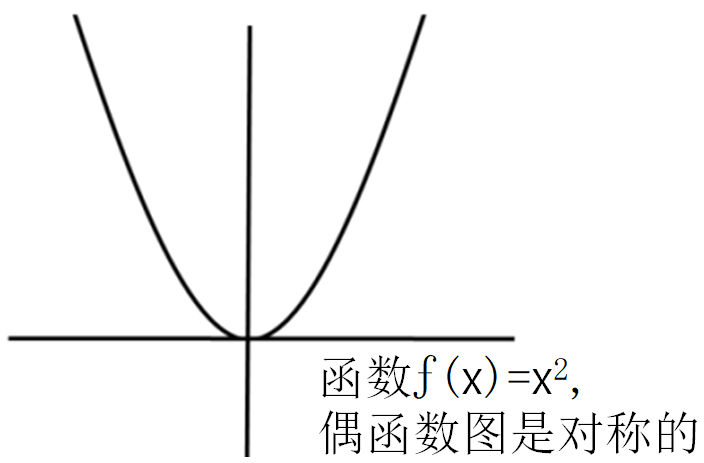
\includegraphics[width=6cm]{./fig/2-1a.png}
    
    (a)
    \end{minipage}
    \begin{minipage}[t]{0.48\textwidth}
    \centering
    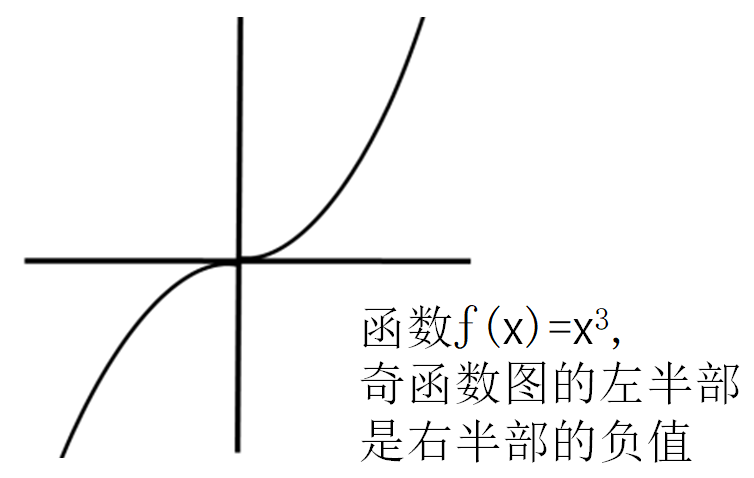
\includegraphics[width=6cm]{./fig/2-1b.png}
    
    (b)
    \end{minipage}
    \caption{偶函数和奇函数}
    \end{figure}

\begin{theorem}
    偶函数在对称区间的积分是在半区间的积分的两倍; \\
    奇函数在对称区间的积分为零。
\end{theorem}

\begin{figure}[htbp]
    \centering
    \begin{minipage}[t]{0.6\textwidth}
    \centering
    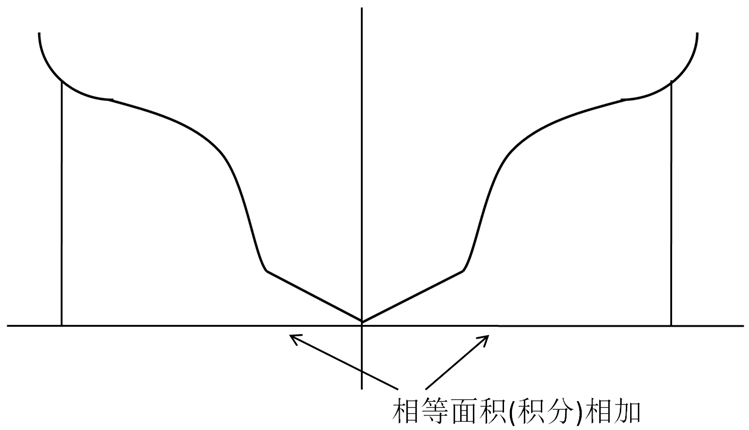
\includegraphics[width=6cm]{./fig/2-2a.png}
    
    (a)偶函数在对称区间的积分为半区间的积分的两倍
    \end{minipage}
    \begin{minipage}[t]{0.6\textwidth}
    \centering
    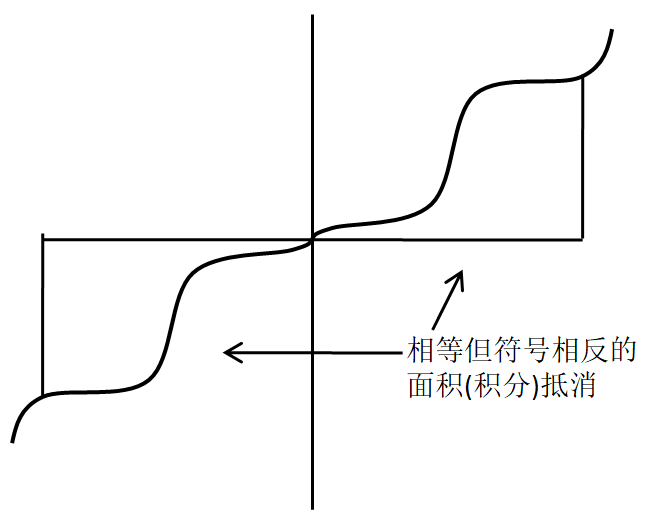
\includegraphics[width=6cm]{./fig/2-2b.png}
    
    (b)奇函数在对称区间的积分为零
    \end{minipage}
    \caption{偶函数和奇函数的积分}
\end{figure}

图2-2示出该定理的图解。可用将整个区间分为二半区间的办法证明:
\[\int_{-a}^a(even)=\int_{-a}^0(even)+\int_0^a(even) \tag{2-11}\]
但因x的偶函数和一x的偶函数一样,所以可用在正半区间$[0,a]$的积分替换在负半区间$[-a,0]$的积分而函数不变:
\[\int_{-a}^a(even)=\int_{-a}^0(even)+\int_0^a(even)=2\int_0^a(even) \tag{2-12}\]
这就证明了定理的第一部分。第二部分的证明也同样简单:
\[\int_{-a}^a(odd)=\int_{-a}^0(odd)+\int_0^a(odd)=-\int_0^a(odd)+\int_0^a(odd)=0 \tag{2-13}\]
奇函数在负半区间的积分可用在正半区间的积分的负值替换。方程2-13给出定理的第二部分。

将此定理应用于对称区间的内积得到另一结果。
\begin{theorem}
    在对称区间$[-a,a]$,奇函數与奇函数或偶函数与偶函数的内积不为零,并可由在半区间$[-a,0]$或$[0,a]$的内积的二倍算出;不论函数是什么形式,偶函数与奇函数的内积为零。
\end{theorem}

在上述五个定义里,我们只考虑了二任意函数。但这些定义的威力和有效性对于函数组无疑也是很明显的。
函数组是函数的集合,它们的变量相同,定义区间相同,和写出函数的规则相同。
例如,x的全部幂函数构成一组函数。
这个函数组用大括号可写
成$\{x^n\}$,它表示这些x的函数的全部:$x^0=1$,$x^1=x$,$x^2$,$x^3$,$x^4$等等。
一般项的指数n表明写出函数组中每个成员的规则。
为了完备起见,必须标明区间和n (常称为指标)可取的值,如下边那样:
“函数组$\{x^n\}$,在$[-1,1]$,$n=0$和全部正整数”。

为了完善地描述量子化学中有用的函数组,我们引人三个新定义。

\begin{definition}[完备函数集]
    完备函数组$\{F_i\}$是这样的函数组,任何别的函数$f$都可在规定的展开区间用函数组$\{F_i\}$的成员线性组合表示,并可达到你所要求的任何精确度
    \footnote{原书的脚注:在这里和以后都默认函数组$\{F_i\}$和函数$f$是均匀连续的,若用了这个概念,则该定义可更严格些,但这在量子化学中是不重要的。}。
\end{definition}

若函数组$\{F_i\}$是完备的,则$f$可展成函数$F_i$.如下:
\[f(x)=a_1F_1(x)+a_2F_2(x)+ \cdots +a_nF_n(x)+ \cdots =\sum_{n=1}^{+\infty}a_nF_n(x) \tag{2-14}\]
一般讲,要证明一函数组是否完备是十分困难的,但根据我们的目的要求,将只考虑已知它们是完备的那些函数组,而不考虑完备性的证明本身。

\begin{definition}[正交完备函数集]
    一函数正交组或正交函数组是这样的函数组,在规定的区间内其中每一函数与全部其它函数都是正交的。
\end{definition}

即若函数组$\{F_i\}$中每一成员与每一其它成员正交,
\[\bra*{F_j}\ket*{F_k}=0 \tag{2-15}\]
对全部j和k$(j \neq k)$,是正交组。
在本章第三节要讨论的函
数组$\{\sin nx,\cos nx\}$在区间$[-\pi,\pi]$,$n=0$或正整数,就是这样的函数组。
证明这些函数组的正交性是本章未要讨论的问题之一;请注意它是三个分开的证明\footnote{作者这里可能想表达三角函数系正交性的三种体现可以分别证明,但对2-16c个人认为改为$\bra*{\sin nx}\ket*{\cos mx}=0 \quad for \ all$ \\ $ \ n,m$更合适,按照原文表述并未完全体现三角函数系的正交性的涵义。}:
\[
\begin{array}{rl}
    \bra*{\sin nx}\ket*{\sin mx}=0 & n \neq m \\
    \bra*{\cos nx}\ket*{\cos mx}=0 & n \neq m \\
    \bra*{\sin nx}\ket*{\cos nx}=0 & for \ all \ n
\end{array}    
\tag{2-16}
\]

最后,将正交性和归性合并在一起。

\begin{definition}[正交归一完备函数集]
    定义正交归一函数组是函数的正交组,其中每一函数又是归一化的。
\end{definition}

即若
\[\bra*{F_j}\ket*{F_k}=0, \ \text{for all} \ j \neq k \tag{2-17a}\]
\[\bra*{F_j}\ket*{F_j}=0, \ \text{for all} \ j=k \tag{2-17b}\]
则$\{F_i\}$是正交归一的。
在讨论正交归一函数时2-17a和2-17b这一对方程要经常出现,因此需要引入一特殊符号将方程2-17a和方程2-17b合并在一起。
克朗尼克符号($\delta_{ij}$)的含义是当$i \neq j$,$\delta_{ij}=0$;当$i=j$,$\delta_{ij}=1$。
若用克朗尼克符号,则正交归一的条件(方程2-17a和方程2-17 b)可简单地表示为
\[\bra*{F_j}\ket*{F_k}=\delta_{ij}, \ \text{for all} \ j,k \tag{2-18}\]
在本章中正交归一组是用小写希腊字母表示,如$\{\phi_i\}$。
在本节中我们定义了一些重要术语,内积,正交性,范数和归一性,完备性,正交和正交归一函数组;我们也应用函数的偶和奇性质简化在对称区间的积分。

\section{用正交归一函数组展开}
在本节中,我们将要学习如何在规定区间将给定函数用一组正交归一函数展开。
因这种演算过程在接着讨论正交归一函数和以后讨论正交归一向量时经常出现,所以先将这些计算公式写出。
\[f(x)=\sum_ia_i\phi_i(x) \tag{2-19}\]
\[\phi_j(x)^*f(x)=\sum_ia_i\phi_j(x)^*\phi_i(x) \tag{2-20}\]
\[\int\phi_j(x)^*f(x)\dd{x}=\sum_ia_i\int\phi_j(x)^*\phi_i(x)\dd{x} \tag{2-21}\]
\[\bra*{\phi_j}\ket*{f}=\sum_ia_i\bra*{\phi_j}\ket*{\phi_i} \tag{2-22}\]
\[\bra*{\phi_j}\ket*{f}=\sum_ia_i\delta_{ji} \tag{2-23}\]
\[\bra*{\phi_j}\ket*{f}=a_j \tag{2-24}\]

方程2- 19表示$f(x)$在特定展开区间(这里未标明)展成正交归一函数组$\{\phi_i\}$的成员的线性组合。
方程2-20是将方程2-19的两端都乘以函数组$\{\phi_i\}$中的任一函数的复共轭$\phi_i(x)^*$的结果。
方程2-21是将方程2- 20的两端在展开区间积分的结果。
而方程2-20和2 21就是$\phi_j$(在左)与方程2-19 (在右)形成的内积。

在方程2-23中根据正交归一的定义以克朗尼克符号$\delta_{ji}$代替$\bra*{\phi_j}\ket*{\phi_i}$。

最后,对方程2-23的右端求和。若将求和写出,则其形式如下:
\[\sum_ia_i\delta_{ji}=a_1\delta_{j1}+a_2\delta_{j2}+ \cdots +a_j\delta_{jj}+ \cdots +a_n\delta_{jn}+ \cdots \tag{2-25}\]

除一个克朗尼克符号外其余的皆为零。仅有的一个不为零的克朗尼克符号是$\delta_{jj}=1$。于是求和给出
\[\sum_ia_i\delta_{ji}=a_j\delta_{jj}=a_j \cdot 1=a_j \tag{2-26}\]

使用在正交归一性基础上产生的克朗尼克符号是在展成正交归一函数时,简化求算系数$a_i$的关键。
方程2-23中的求和遵守一简单的规则:在对包含克朗尼克符号和别的量的乘积求和时,只挑选出包含下标相同的克朗尼克符号的项就行,或只剩下包含下标相同的克朗尼克符号的项。

最后,方程2-24是在给定区间将一函数展成正交归一函数组的展开系数的计算公式,$a_j=\bra*{\phi_j}\ket*{f}$。展开系数可以是复数。
不要用错下标!若需要$a_1$,就要求算$\bra*{\phi_1}\ket*{f}$,需要$a_2$,就求算$\bra*{\phi_2}\ket*{f}$;需要$a_3$,就求算$\bra*{\phi_3}\ket*{f}$,以此类推。下节我们将详细地举一例。

下边我们转入一在实用上重要的问题。若将展成正交归一组的展开式中若干项后各项断掉,产生的误差是多少?
在回答此问题中显现出展开系数的一个新性质:这些系数可使断尾展开式的误差极小。用$M_n$表示取n项的误差。此误差可用下式求出\footnote{原书的脚注:这是误差的“最小二乘法”判别。别的方法也可以用。还应注意,如果整个函数是归一化的,则断尾展开式不是归一化的。};
\[M_n=\int\abs\Big{f(x)-\sum_{j=1}^nb_j\phi_j}^2\dd{x} \tag{2-27}\]

即,用余项的绝对值的平方与x对划的曲线下的面积求算。
积分范围是展开区间。在图2-3中用图说明$M_n$的含义。因$c^*c=\abs*{c}^2$,故可写成
\[M_n=\int \left ( f^*-\sum_{j=1}^nb_j^*\phi_j^* \right ) \left ( f-\sum_{i=1}^nb_j\phi_j \right )\dd{x}\]
\[=\bra*{f}\ket*{f}-\sum_{j=1}^nb^*_j\bra*{\phi_j}\ket*{f}-\sum_{i=1}^nb_j\bra*{f}\ket*{\phi_j}+\sum_{j=1}^n\sum_{i=1}^nb_j^*b_i\bra*{\phi_j}\ket*{\phi_i} \tag{2-28}\]

注意方程2-28中每个因式所用的求和指标不同。求和指标常常只是傀标,因为它们的名称单独存在并无什么特殊意义。然而,对它们的名称却必须时常小心地加以辨别。例如,
\[\left (\sum_ic_i\phi_i\right )\left (\sum_ic_i\phi_i\right )\]
可能误写为
\[\sum_ic_i^2\phi_i^2\]
\begin{figure}[htbp]
    \centering
    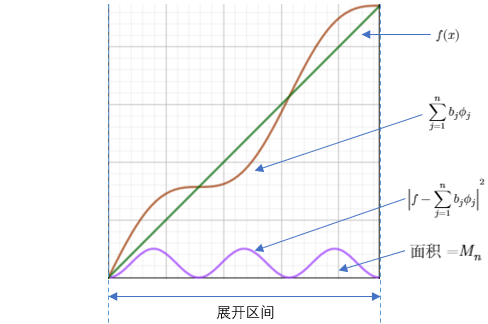
\includegraphics[scale=0.6]{./fig/2-3.png}
    \caption{展成正交归一函数的断尾展开的误差}
\end{figure}
但它不是乘积的含义。若加和写出,$(c_1\phi_1+c_2\phi_2+ \cdots )(c_1\phi_1+c_2\phi_2+ \cdots )$等于$c_1^2\phi_1^2+c_1c_2\phi_1\phi_2+c_2c_1\phi_2\phi_1+c_2^2\phi_2^2 \cdots $,它与
\[\sum_ic_i^2\phi_i^2=c_1^2\phi_1^2+c_2^2\phi_2^2+ \cdots\]
差别很大。为了保证写出的答案正确(包含交错项),我们使用下列符号
\[\left (\sum_ic_i\phi_i\right )\left (\sum_jc_j\phi_j\right )=\sum_{ij}c_ic_j\phi_i\phi_j\]

因函数组$\{\phi_i\}$是正交归一的,所以方程2-28的末项中可代入克朗尼克符号\footnote{原书合并后最后一项连加的符号误写为+。}:
\[M_n=\bra*{f}\ket*{f}-\sum_{j=1}^nb^*_j\bra*{\phi_j}\ket*{f}-\sum_{i=1}^nb_j\bra*{f}\ket*{\phi_j}+\sum_{j=1}^n\sum_{i=1}^nb_j^*b_i\delta_{ij}\]
\[=\bra*{f}\ket*{f}-\sum_{j=1}^n \left ( b^*_j\bra*{\phi_j}\ket*{f}+b_j\bra*{f}\ket*{\phi_j}-b_j^*b_j \right ) \tag{2-29}\]

在包含克朗尼克符号的项中对$i$求和,只剩下$i=j$的项,又因求和指标的名称不重要,故三项都用指标$j$表示,并且并在一起。

我们可借助使与系数$b_j$对应的误差$M_n$极小的办法求展开系数的“最佳”组。
因为$b_j$,有实数和虚数两部分,所以它包含两步。
双极小问题可表为对全部$j$求$\partial M_n / \partial b_j=\partial M_n / \partial b_j^*=0$。
对方程2-29求导数得出
\[\frac{\partial M_n}{\partial b_j}=0=-\bra*{f}\ket*{\phi_j}+b^*_j \tag{2-30a}\]
\[\frac{\partial M_n}{\partial b_j^*}=0=-\bra*{\phi_j}\ket*{f}+b_j \tag{2-30b}\]
这两个方程彼此成复共轭,从使误差为极小的意义看,展开式的“最佳”系数可由下式求出:
\[b_j=\bra*{\phi_j}\ket*{f} \tag{2-31}\]
由方程2-31得出的系数事实上就是展成正交归一函数时必须使用的系数。
因此,$a_j=b_j=\bra*{\phi_j}\ket*{f}$\footnote{这里莫名其妙的换了系数的符号我猜是作者同时参考了两本书发现符号不同但是懒得改了(笑)。}不仅是 “正确”的系数(方程2-24),而且也是“最佳”的系数(方程2-31)。

将$a_j=b_j=\bra*{\phi_j}\ket*{f}$代入方程2-29,求出的误差为
\[M_n=\bra*{f}\ket*{f}-\sum_{j=1}^n \left ( a_ja_j^*+a_j^*a_j-a_j^*a_j \right )=\bra*{f}\ket*{f}-\sum_{j=1}^n\abs*{a_j}^2 \tag{2-32}\]

我们用一个称为展开定理的有关内积的重要关系结束本节。

\begin{theorem}
    内积$\bra*{f}\ket*{g}$可 用正交归一函数组$\{\phi_i\}$展开为
    \[\bra*{f}\ket*{g}=\sum_i\bra*{f}\ket*{\phi_i}\bra*{\phi_i}\ket*{g} \tag{2-33}\]
\end{theorem}

为了证明此定理,可将$f$展成$f=\sum_ia_i\phi_i$,$g$展成$g=\sum_ib_i\phi_i$。于是
\[\bra*{f}\ket*{g}=\int f^*g=\sum_i\sum_j\int a^*_i\phi_J^*b_j\phi_j=\sum_{ij}a_i^*b_j\bra*{\phi_i}\ket*{\phi_j}=\sum_{ij}a_i^*b_j\delta_{ij}\]
而
\[a_i^*=\bra*{\phi_i}\ket*{f}^*=\bra*{f}\ket*{\phi_i},b_i=\bra*{\phi_i}\ket*{g}\]
因此,
\[\bra*{f}\ket*{g}=\sum_i\bra*{f}\ket*{\phi_i}\bra*{\phi_i}\ket*{g}\]

展开定理中出现的结构$\ket*{\phi_i}\bra*{\phi_i}$在本书后边将赋予更多的含义。
现在我们在展开定理中看到的只是在$\bra*{f}$和$\ket*{g}$之间插入$\ket*{\phi_i}\bra*{\phi_i}$对$i$求和。
这就是实际情况;这种运算称为“插入态的完备组”。
展开定理可写成$\sum\ket*{\phi_i}\bra*{\phi_i}=1$。
结构$\ket*{\phi_i}\bra*{\phi_i}$不是方程2-29定义的内积,它是我们到此为止还未讨论的一个元素。
它实际上是一个算符。以后会明显地看到它起着算符的作用。

在本节中,我们导出了展成正交归一函数组的展开式中系数公式;证明了这些系数使断尾展开式的误差极小,并导出断掉展开式\footnote{我觉得叫断尾展开式或者截尾展开式都比这个好。}的余项产生的误差公式。最后,导出内积的展开定理。

\section{富里叶(Fourier)级数}

富里叶级数\footnote{古早翻译了属于是。}是将函数展成与${\sin mx,\cos \, mx}$成比例的正交归一函数组的展开式。
在第一节中讲过这些函数是正交的,现在导出它在$[-\pi,\pi]$区间的范数。
\[N(\sin mx)=\bra*{\sin mx}\ket*{\sin mx}=\int_{-\pi}^{\pi}\sin^2 \, mx\dd{x}=\frac{1}{m}\int_{-m\pi}^{m\pi}\sin^2y\dd{y}=\pi \tag{2-34}\]
同样
\[N(\cos mx)=\bra*{\cos mx}\ket*{\cos mx}=\int_{-\pi}^{\pi}\cos ^2 \, mx\dd{x}=\frac{1}{m}\int_{-m\pi}^{m\pi}\cos ^2y\dd{y}=\pi \tag{2-35}\]
方程2-34和2-35除m=0外对全部m值都成立,而m=0时则得出不定的N=0/0。为了澄清m=0的情况,必须分开求算
\[N(\sin \, 0x)=\bra*{\sin \, 0x}\ket*{\sin \, 0x}=\int_{-\pi}^{\pi}0\dd{x}=0 \tag{2-36}\]
\[N(\cos  \, 0x)=\bra*{\cos  \, 0x}\ket*{\cos  \, 0x}=\int_{-\pi}^{\pi}1\dd{x}=2\pi \tag{2-37}\]
全部结果可以表为
\[
N(\sin mx)=\left\{
\begin{array}{rl}
    \pi, & m \neq 0 \\
    0, & m=0
\end{array}
\right.
\qquad
N(\cos mx)=\left\{
\begin{array}{rl}
    \pi, & m \neq 0 \\
    2\pi, & m=0 \\
\end{array}  
\right.  
\tag{2-38a}
\]
或用克朗尼克符号表示
\[
\begin{array}{c}
    N(\sin mx)=\pi-\pi \delta_{m0} \\
    N(\cos mx)=\pi+\pi \delta_{m0}
\end{array}    
\tag{2-38b}
\]
与正交关系式合在一起,可写出$(\sin mx ,\cos mx)$的全部可能的内积
\[
\begin{array}{c}
    \bra*{\sin mx}\ket*{\cos mx}=0 \\
    \bra*{\sin mx}\ket*{\sin nx}=(1-\delta_{m0})\pi \delta_{mn} \\
    \bra*{\cos mx}\ket*{\cos nx}=(1+\delta_{m0})\pi \delta_{mn}
\end{array}    
\tag{2-39}
\]

对全部m,n为任意正整數或零。因为我们要用以前的公式(方程2-24)来计算展成正交归一函数组的展开系数,所以必须用函数组
$\{(2\pi)^{-\frac{1}{2}},(\pi)^{-\frac{1}{2}}\sin mx,(\pi)^{-\frac{1}{2}}\cos mx\}$, $m=1,2,\cdots $,$[-\pi,\pi]$代替函数组${\sin mx ,\cos mx}$。

对于这些正交归一函数,展开系数为
\[
\begin{array}{c}
    a_0=\bra*{\frac{1}{\sqrt{2\pi}}}\ket*{f} \\
    a_m=\bra*{\frac{\cos mx}{\sqrt{\pi}}}\ket*{f} \\
    b_m=\bra*{\frac{\sin mx}{\sqrt{\pi}}}\ket*{f}
\end{array}    
\tag{2-40}
\]
展开式为
\[f(x)=\frac{a_0}{\sqrt{2\pi}}+\sum_{m=1}^{+\infty}\frac{a_m}{\sqrt{\pi}}\cos mx+\sum_{m=1}^{+\infty}\frac{b_m}{\sqrt{\pi}}\sin mx \tag{2-41}\]
这不是富里叶级数的一般形式,只是展成正交归一函数组的一个例子。一般是利用以显式写出展开系数的办法将常数移到项外:
\[f(x)=\frac{\bra*{1}\ket*{f}}{2\pi}+\frac{1}{\pi}\sum_{m=1}^{+\infty}(\bra*{\cos mx}\ket*{f}\cos mx+\bra*{\sin mx}\ket*{f}\sin mx) \tag{2-42}\]
最终的结果是
\[f(x)=\frac{c_0}{2}+\sum_{m=1}^{+\infty}c_m\cos mx+\sum_{m=1}^{+\infty}d_m\sin mx \tag{2-43}\]
\[c_m=\frac{1}{\pi}\bra*{\cos mx}\ket*{f} \tag{2-44a}\]
\[d_m=\frac{1}{\pi}\bra*{\sin mx}\ket*{f} \tag{2-44b}\]
在$[-\pi,\pi]$区间。这是富里叶级数常用的形式。注意首项被2除。
这是因为$\cos  \, 0x$的范数是2π,对其它全部m值,$\cos mx$的范数是π。

我们能用偶函数和奇函数的性质立刻做出富里叶级数的两个简单推论。
正弦函数是奇函数:$\sin\, x=-\sin(-x)$。余弦函数是偶函数:$\cos  \, x=\cos (-x)$。因此,我们可以写出两个规则。

(1)一奇函数在$[-\pi,\pi]$区间的富里叶展开仅由正弦项组成:$f(x)=\sum d_m\sin mx$。
(1)一偶函数在$[-\pi,\pi]$区间的富里叶展开仅由余弦项组成:$f(x)=\sum c_m\cos mx$。
因为若f是奇函数,则所有内积$\bra*{\cos mx}\ket*{f}=0$;
若f是偶函数,则所有内积$\bra*{\sin mx}\ket*{f}=0$。
例

$f(x)=x$在$[-\pi,\pi]$的展开。因$f(x)=x$是奇函数,所以仅正弦项存在,因此可写成
\[x=\sum_{m=1}^{+\infty}d_m\sin mx, \ m=1,2, \cdots \ in \ [-\pi,\pi]\]
式中
\[d_m=\frac{1}{\pi}\bra*{\sin mx}\ket*{x}=\frac{1}{\pi}\int_{-\pi}^{\pi}x\sin \,mx\dd{x}=\frac{1}{m^2\pi}\int_{-m\pi}^{m\pi}y\sin y\dd{y}=\eval{\frac{1}{m^2\pi}(-y\cos y+\sin y)}_{-m\pi}^{m\pi}\]
\[=-\frac{m\pi \cos  \, m\pi+m\pi \cos  \,m\pi}{m^2\pi}=\frac{2(-1)^{m+1}}{m}\]
富里叶级数为
\[x=\sum_{m=1}^{+\infty}\frac{2(-1)^{m+1}}{m}\sin mx=2\sin \, x-\sin \, 2x +\frac{2}{3}\sin \, 3x -\cdots\]

三项后断尾的富里叶级数和函数本身的比较示于图2-4。可利用方程2-32求出取三项的富里叶级数的均方误差如下:
\[M_3=\bra*{x}\ket*{x}-\sum_{j=1}^3\abs*{a_j}^2 \tag{2-45}\]
根据方程2-40和2-44,$a_j=\sqrt{\pi}d_j$,可得
\[M_3=\int_{-\pi}^{\pi}x^2\dd{x}-4\pi-1\pi-\frac{4}{9}\pi=\frac{2\pi^3}{3}-\frac{49\pi}{9} \approx 6.8\]
其平方根为2.6,可与函数下的面积$\pi^2=9.9$比较。因此,断掉三项后的余项造成的相对误差约为26\%。

\begin{figure}[htbp]
    \centering
    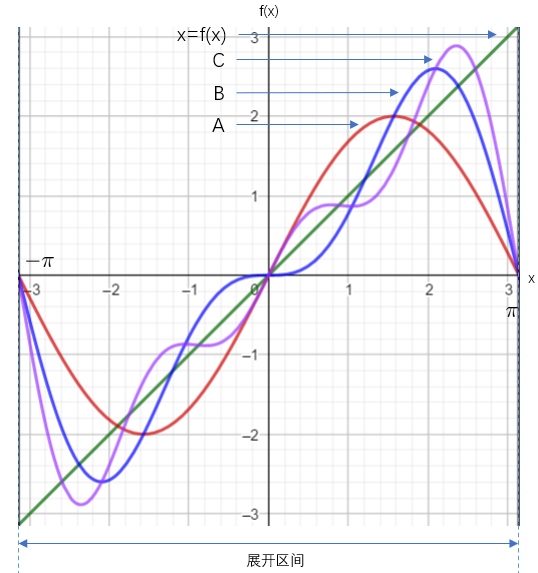
\includegraphics[scale=0.4]{./fig/2-4.png}
    \caption{在区间$[-\pi,\pi]$的函数$f(x)=x$及其富里叶级数展开(A)一项,(B)两项,(C)三项}
\end{figure}

用富里叶级数描述函数有一重要的电子学类比。在通常情况下,很容易在电路中发生正弦和余弦函数。
也可用电子学中的富里叶合成发生其它函数。用这种合成可发生如图2-5a所示的所谓“锯齿”波。
锯齿波是在$[-\pi,\pi]$区间无穷级数$f(x)=x$与对划得到的图,它具有前例中导出的富里叶组分。
图2-5b表示锯齿波的三项近似图。这样的波形被用于示波器和电视中扫描。

\begin{figure}[htbp]
    \centering
    \begin{minipage}[t]{0.7\textwidth}
    \centering
    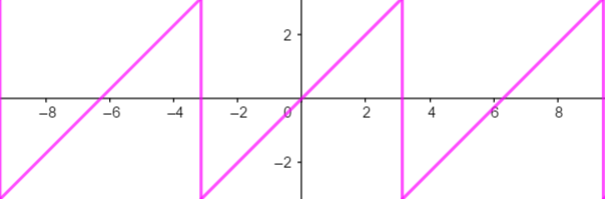
\includegraphics[width=8cm]{./fig/2-5a.png}
    
    (a)
    \end{minipage}
    \begin{minipage}[t]{0.7\textwidth}
    \centering
    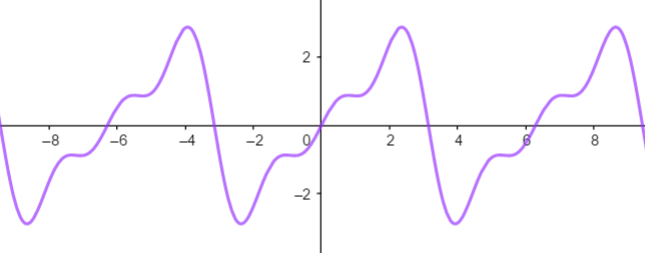
\includegraphics[width=8cm]{./fig/2-5b.png}
    
    (b)
    \end{minipage}
    \caption{(a)“锯齿”波 \quad (b)锯齿波的三项富里叶合成}
\end{figure}

函数$\{\sin mx\}$和$\{\cos mx\}$无论在半区间$[-\pi,0]$或$[0,\pi]$中都是完备的。
这些函数在哪个半区间也都是正交的。
除$\cos  \, 0x$的范数是$\pi$外,所有其它函数的范数都是$\frac{\pi}{2}$因此,我们能够造两个不同的“半富里叶级数”:
\[f(x)=\frac{c_0}{2}+\sum_{m=1}^{+\infty}c_m\cos mx \qquad c_m=\frac{2}{\pi}\bra*{\cos mx}\ket*{f} \tag{2-46}\]
\[f(x)=\sum_{m=1}^{+\infty}d_m\sin mx \qquad d_m=\frac{2}{\pi}\bra*{\sin mx}\ket*{f} \tag{2-47}\]
它们的展开区间都是$[-\pi,0]$或$[0,\pi]$。
无论全富里叶级数还是半富里叶级数都可用按比例展开的办法推广到任何对称区间
$[-a,a]$或半对称区间$[-a,0]$或$[0,a]$,如
\[f(x)=\frac{c_0}{2}+\sum_{m=1}^{+\infty} \left ( c_m\cos \frac{m\pi x}{a}+d_m\sin\frac{m\pi x}{a} \right ) \tag{2-48}\]
\[c_m=\frac{1}{a}\bra*{\cos \frac{m\pi x}{a}}\ket*{f} \qquad d_m=\frac{1}{a}\bra*{\sin\frac{m\pi x}{a}}\ket*{f}\]
在量子力学中富里叶级数的一个重要的经过修正的形式为\footnote{这个形式的强大之处在于它是复数域的傅里叶变换,但一般量子化学不太涉及复变函数的运算,以至于大部分人直接只把它认成一般实数域下的傅里叶变换的简洁形式。}
\[f(x)=\sum_{m=-\infty}^{+\infty}a_me^{imx} \qquad x \in [-\pi,\pi] \tag{2-49}\]
因为若$\{\sin mx,\cos mx\}$对全部正m值和零是完备的,则${e^{imx}=\cos mx + i\sin mx}$对m的全部整数值(正,负和零)也是完备的。
可将函数组$\{e^{imx}\}$的复共轭包括在内,以使函数组完备。
基本富里叶级数的这些修正形式是本章末许多问题中要讨论的课题。

本节展示了非常有用的正交归一函数组展开,富里叶级数(展成正弦和余弦函数),并对它的用途和适用范围做了评论。

\section{构造正交归一函数}
到目前为止我们已一般地讨论了正交归一函数组的性质,它们在级数展开中的应用,以及富里叶级数这个特殊例子。
我们曾经指出,无论正交归一否,唯有函数组是完备的才能得到足够精确的展开。
本节将介绍如何由一完备函数组形成完备正交归函数组。
在实际造完备正交归一函数前,必须引入与完备性有关的一个问题,此问题在目前的讨论和紧接着的工作中都起着重要作用。
我们从一个定义开始。

\begin{definition}[线性无关,线性相关]
    若一函数组中任一函数都不能用其余函数的线性组合来表示,则称该函数组为线性无关的。同样的,若至少有一函数可以线性方程与一个或多个其它函数关联,则称该函数组为线性相关的。
 \end{definition}
此定义可用数学公式表示为,若方程
\[\sum_iC_iF_i=C_1F_1+C_2F_2+ \cdots \tag{2-50}\]
仅当所有的$C_i=0$时才可解,则函数组$\{F_i\}$是线性无关的。若该方程在至少有一个$C_i \neq 0$时可解,则$\{F_i\}$是线性相关的。取下列两组函数为例:
\[
\begin{array}{ll}
    F_1=1 & G_1=1 \\
    F_2=x & G_2=x \\
    F_3=7x+4 & G_3=x^3 \\
    F_4=x^3 & G_4=x^3
\end{array}    
\]
函数组$\{G_i\}$是线性无关的。不可能使这些函数的任何线性组合如方程2-50那样为零。
另一种说法是,这四个函数没有线性关系:$G_3=x^2$不是$1$, $x$和$x^3$的线性组合。$\{F_i\}$是线性相关的。$F_3$是$F_1$,$F_2$和$F_4$的线性组合;$F_3=7F_2+4F_1$。
即方程2-50可在有些$C_i \neq 0$时解出;$-4F_1-7F_2+1F_3+0F_4=0$。

一完备函数组总是包含一线性无关子集(亚组)。这是我们未做证明的一个重要表述;它是造完备正交归一函数组的第一步。

我们用在$[-1,1]$区间x的幂函数为例。泰勒定理从根本上保证函数组$\{x^n\}$,$n=0,1,2 \cdots $,是完备的。
我们也已看到这些函数是线性无关的。再看下列函数组。$\{F'_i\}$是完备的;可从$\{F'_i\}$中将线性相关的组分移出而形成线性无关的函数组$\{F_i\}$。
$\{G_i\}$也是线性无关的和完备的;它与$\{F_i\}$的差别仅仅是排列次序不同。

\[
\begin{array}{ccc}
    \{F'_i\} & \{F_i\} & \{G_i\} \\
    1 & 1 & 1 \\
    x & x & x^2 \\
    2x & \cdots & x^4 \\
    x^2 & x^2 & \cdots \\
    x^3 & x^3 & x \\
    x^4 & x^4 & x^3 \\
    \cdots & \cdots & \cdots
\end{array}    
\]

总是可以从一完备的线性无关的函数组造一完备的正交归一函数组。造正交归一函数组的方法称为施密特正交化。
我们不准备对该方法作全面介绍,只想讲清楚概念,叙述一般结论,然后举一例说明之。
假定有一定义在特定区间的完备的,线性无关的函数组$\{f_i\}$。我们希望用$\{f_i\}$造一正交归一函数组$\{\phi_i\}$。

第一步,令$\phi_0$为归一化的$f_0$。即,使第一个$\phi$函数只与第一个$f$函数成比例。
$f_0$的范数是$N_0=\bra*{f_0}\ket*{f_0}$,因此,$\phi_0=f_0/\sqrt{N_0}$。

第二步,令$\phi_1$为$\phi_0$和$f_1$的线性组合,它与$\phi_0$正交,且是归一化的。 
因$\{f_i\}$是线性无关的所以一般讲这是办的到的。即,
\[\phi_1=\frac{1}{\sqrt{N_1}}(c\phi_0+f_1) \tag{2-50}\]
\[\bra*{\phi_0}\ket*{\phi_1}=0 \tag{2-51}\]
正交条件给出
\[c\bra*{\phi_0}\ket*{\phi_0}+\bra*{\phi_0}\ket*{f_1}=0 \tag{2-53a}\]
\[c=-\bra*{\phi_0}\ket*{f} \tag{2-53b}\]
于是,
\[\phi_1=\frac{1}{\sqrt{N_1}}(f_1-\bra*{\phi_0}\ket*{f_1}\phi_0) \tag{2-54}\]
和
\[N_1=\bra*{f_1}\ket*{f_1}-\bra*{\phi_0}\ket*{f_1}\bra*{f_1}\ket*{\phi_0}-\bra*{\phi_0}\ket*{f_1}\bra*{\phi_0}\ket*{f_1}+\bra*{\phi_0}\ket*{f_1}^2=\bra*{f_1}\ket*{f_1}-\abs*{\bra*{\phi_0}\ket*{f_1}}^2 \tag{2-55}\]

这种步骤一直继续到完备的正交归一函数组造好为止。一般项为
\[\phi_k=\frac{1}{\sqrt{N_k}} \left ( f_k-\sum_{j=0}^{k-1}\bra*{\phi_j}\ket*{f_k}\phi_j \right ) \tag{2-56}\]
\[N_k=\bra*{f_k}\ket*{f_k}-\sum_{j=0}^{k-1}\abs*{\bra*{\phi_j}\ket*{f_k}}^2 \tag{2-57}\]

从讨论中应该搞清楚,如果函数的范数不是有限值,则这些函数就不能归一化。
并非所有函数在所有区间内都是可归一化的;如,函数组$\{x^n\}$在$[-\infty,\infty]$就不是可归一化的。
分子结构的量子力学涉及的函数组几乎都是可归一化的,或平方可积的。

取在全区间$[-\infty,\infty]$函数组$\{x^ne^{-\frac{1}{2}x^2}\}$\footnote{原书中这个函数集的形式写成了$\{e^{-\frac{1}{2}x^2}x^n\}$,我觉得不好看所以给他换过来了。}做为施密特正交化的例子。先证明这些函数是可归一化的。
\[\bra*{f_n}\ket*{f_n}=\int_{-\infty}^{+\infty}e^{-\frac{1}{2}x^2}x^ne^{-\frac{1}{2}x^2}x^n\dd{x}=\int_{-\infty}^{+\infty}e^{-x^2}x^{2n}\dd{x} \tag{2-58}\]
因为被积函数是偶函数,故可使积分简化为
\[\bra*{f_n}\ket*{f_n}=2\int_{0}^{+\infty}e^{-x^2}x^{2n}\dd{x}=\int_{0}^{+\infty}e^{-y}y^{n-\frac{1}{2}}\dd{y} \tag{2-59}\]
用部分积分连续积分给出
\[\bra*{f_n}\ket*{f_n}=\left ( n-\frac{1}{2} \right )\left ( n-\frac{3}{2} \right ) \cdots \left ( \frac{1}{2} \right )\int_{0}^{+\infty}e^{-y}y^{-\frac{1}{2}}\dd{y}\]
\[=2\left ( n-\frac{1}{2} \right )\left ( n-\frac{3}{2} \right ) \cdots \left ( \frac{1}{2} \right )\int_{0}^{+\infty}e^{-x^2}\dd{x}\]
\[=(2n-1)(2n-3) \cdots (3)(1)\frac{\sqrt{\pi}}{2^n} \tag{2-60}\]
式中是将已知积分$\int_0^{+\infty}e^{-x^2}\dd{x}=\frac{\sqrt{\pi}}{2}$代入。对所有的n,范数$N_n$都是有限值。
因此$\{e^{-\frac{1}{2}x^2}x^n\}$中所有函数都是可归一化的。
衰减指数函数$e^{-\frac{1}{2}x^2}$的存在使积分是有限的和函数是平方可积的。

要造正交归一函数组,先将$f_0=e^{-\frac{1}{2}x^2}x^0=e^{-\frac{1}{2}x^2}$归化。
其范数为$\sqrt{\pi}$,故得到$\phi_0=\pi^{-\frac{1}{4}}e^{-\frac{1}{2}x^2}$。
用方程2-54和2-55求下一个函数,它是方程2-56和2-57的特殊情况。
为了使用这些方程,必须先求出$\bra*{\phi_0}\ket*{f_1}$和$\bra*{f_1}\ket*{f_1}$。因被积函数是奇函数,故
\[\bra*{\phi_0}\ket*{f_1}=\int_{-\infty}^{\infty}\pi^{-\frac{1}{4}}e^{-\frac{1}{2}x^2}e^{-\frac{1}{2}x^2}x^1\dd{x}=0 \tag{2-61}\]
根据方程2-60,
\[\bra*{f_1}\ket*{f_1}=\frac{\sqrt{\pi}}{2} \tag{2-62}\]
于是
\[N_1=\bra*{f_1}\ket*{f_1}-\abs*{\bra*{\phi_0}\ket*{f_1}}^2=\frac{\sqrt{\pi}}{2} \tag{2-63}\]
和
\[\phi_1=\frac{1}{\sqrt{N_1}}(f_1-\bra*{\phi_0}\ket*{f_1}\phi_0)=\left ( \frac{2^2}{\pi} \right )^{\frac{1}{4}}xe^{-\frac{1}{2}x^2} \tag{2-64}\]

读者应看到,因被积函数是奇函数,故对这组函数所有形式为$\bra*{\phi_i}\ket*{f_j}$(i是偶数,是奇数,或相反)的积分都是零。这使计算大大简化。

根据方程2-56和2-57,下一个函数可计算如下:
\[\phi_2=\frac{1}{\sqrt{N_2}}(f_2-\bra*{\phi_0}\ket*{f_2}\phi_0-\bra*{\phi_1}\ket*{f_2}\phi_1)=\frac{1}{\sqrt{N_2}}(f_2-\bra*{\phi_0}\ket*{f_2}\phi_0) \tag{2-65}\]
\[N_2=\bra*{f_2}\ket*{f_2}-\abs*{\bra*{\phi_0}\ket*{f_2}}^2-\abs*{\bra*{\phi_1}\ket*{f_2}}^2=\bra*{f_2}\ket*{f_2}-\abs*{\bra*{\phi_0}\ket*{f_2}}^2 \tag{2-66}\]
需要计算$\bra*{f_2}\ket*{f_2}$和$\bra*{\phi_0}\ket*{f_2}$,从方程2-60,
\[\bra*{f_2}\ket*{f_2}=\frac{3}{4}\sqrt{\pi} \tag{2-67}\]
和
\[\bra*{\phi_0}\ket*{f_2}=\int_{-\infty}^{\infty}\pi^{-\frac{1}{4}}e^{-\frac{1}{2}x^2}e^{-\frac{1}{2}x^2}x^2\dd{x}=\pi^{-\frac{1}{4}}\int_{-\infty}^{\infty}x^2e^{-x^2}\dd{x}=\pi^{-\frac{1}{4}}\frac{\sqrt{\pi}}{2}=\frac{\pi^{\frac{1}{4}}}{2} \tag{2-68}\]
最后得出,
\[N_2=\frac{3}{4}\sqrt{\pi}-\frac{1}{4}\sqrt{\pi}=\frac{1}{2}\sqrt{\pi} \tag{2-69}\]
\[\phi_2=\left( \frac{2^2}{\pi}\right)^{\frac{1}{4}}\left( x^2e^{-\frac{1}{2}x^2}-\frac{\pi^{\frac{1}{4}}}{2} \cdot \frac{1}{\pi^{\frac{1}{4}}}e^{-\frac{1}{2}x^2}\right)=\left( \frac{1}{\pi}\right )^{\frac{1}{4}}\frac{2x^2-1}{\sqrt{2}}e^{-\frac{1}{2}x^2} \tag{2-70}\]

用这种方法造的正交归一.函数组的形式是$\pi^{-\frac{1}{4}}H_n(x)e^{-\frac{1}{2}x^2}$,式中$H_n(x)$表示下列多项式之一,
\[H_0(x)=1 \qquad H_1(x)=x \qquad H_2(x)=\frac{2x^2-1}{\sqrt{2}} \qquad \cdots  \tag{2-71}\]

偶数多项式只包含x的偶次幂,奇数多项式只包含奇次幂。这些多项式与著名的厄米多项式成比例。\footnote{这些多项式就是在对应的厄米多项式上多除了一个系数$\sqrt{2^nn!}$。}
我们用函数组$\{x^ne^{-\frac{1}{2}x^2}\}$造的在$[-\infty,\infty]$区间的正交归一函数组是量子力学谐振子的波动方程的解。
当然,在造这些函数时我们并未注意任何特殊物理问题。
沿这个路线走,我们偶然逢到物理问题的解这样的事,加强了量子力学中谐振子的意义和简明性。

这样,我们在本节中用线性无关和可归一化的概念进一步展开了函数的性质,并介绍了如何由一完备的线性无关丽数组,造宗备的正交归一函数组。
最后, 我们开始粗略地将正交归函数与描述物理状态的波函数联系起来。

\section{勒让德多项式和其它特殊函数}

在本节中我们要考察在不同区间的一些正交归一函数组。这可能是一项庞大的工作。
这样函数间的关系式在较大部头的著作中都以表的形式列出,同时这些关系式的证明在量子化学中也不重要。
因此,本节着重考察一个特殊函数(勒让德多项式),并粗略地列出包括拉基尔函数和厄米函数在内的其它函数。
在很多量子化学问题中勒让德多项式很重要。
它是角动量波函数的基础,因此出现在球形运动的问题中,诸如氢原子中的电子运动或分子的转动。
勒让德多项式在描述单电子轨道的角度部分很重要;而角动量部分又形成化合物的几何学的基础。

形成这些多项式的方法很多,其中有三种是常用的。

(a)线性无关的完备函数组的施密特正交化。

(b)解微分方程。

(c)使用母函数。

此外,我们还要讲勒让德($Rodrigues$)多项式的一个公式。先讨论正交化。

\paragraph*{用施密特正交化造勒让德多项式}对在区间$[-1,1]$的函数组$\{x^n\}$进行施密特正交化可以得到勒让德多项式。
选择$[-1,1]$区间对勒让德多项式是特有的。
先令$\phi_0$与$x^0=1$成比例,并在该区间归一化:
\[N_0=\int_{-1}^1\dd{x}=2 \tag{2-72}\]
\[\phi_0=\sqrt{\frac{1}{2}} \tag{2-73}\]
再用方程2 -56和2-57,得出
\[N_1=\bra*{f_1}\ket*{f_1}-\abs*{\bra*{\phi_0}\ket*{f_1}}^2=\bra*{f_1}\ket*{f_1}=\int_{-1}^1x^2\dd{x}=\frac{2}{3} \tag{2-74}\]
\[\phi_1=\frac{1}{\sqrt{N_1}}(f_1-\bra*{\phi_0}\ket*{f_1}\phi_0)=\sqrt{\frac{3}{2}} \tag{2-75}\]
由于被积函数是奇函数,所以$\bra*{\phi_0}\ket*{f_1}=0$;同样,其下标的和是奇数的所有内积皆为零。这种行为在前节的厄米多项式中已经见过。

继续进行下去,可求出
\[N_2=\bra*{f_2}\ket*{f_2}-\abs*{\bra*{\phi_0}\ket*{f_2}}^2 \tag{2-76}\]
\[\phi_2=\frac{1}{\sqrt{N_2}}(f_2-\bra*{\phi_0}\ket*{f_2}\phi_0) \tag{2-77}\]
需要计算
\[\bra*{f_2}\ket*{f_2}=\int_{-1}^1x^4\dd{x}=\frac{2}{5} \tag{2-78}\]
\[\bra*{\phi_0}\ket*{f_2}=\int_{-1}^1\frac{1}{\sqrt{2}}x^2\dd{x}=\sqrt{\frac{1}{2}} \cdot \frac{2}{3} \tag{2-79}\]
由此得出
\[N_2=\frac{2}{5}-\frac{1}{2} \cdot \frac{4}{9}=\frac{8}{45} \tag{2-80}\]
\[\phi_2=\sqrt{\frac{45}{8}} \cdot \left(x^2-\frac{1}{3}\right)=\sqrt{\frac{5}{2}} \cdot \left(\frac{3}{2}x^2-\frac{1}{2}\right) \tag{2-81}\]
这些函数的形状是
\[\phi_0=\sqrt{\frac{1}{2}} \cdot 1\]
\[\phi_1=\sqrt{\frac{3}{2}} \cdot x\]
\[\phi_2=\sqrt{\frac{5}{2}} \cdot \left(\frac{3}{2}x^2-\frac{1}{2}\right)\]
\[\phi_4=\sqrt{\frac{7}{2}} \cdot \left(\frac{5}{2}x^3-\frac{3}{2}x\right) \tag{2-82}\]
右边的多项式就是勒让德多项式,整个正交归一函数组是$\{\sqrt{\frac{2n+1}{2}}P_n(x)\}$,式中$P_n(x)$表示n次勒让德多项式。

\paragraph*{解勒让德微分方程}勒让德多项式是下列微分方程的解:
\[\dv{x} \left [(1-x^2) \dv{f}{x} \right ]+l(l+1)f=0 \tag{2-83}\]
式中$l$是正整数或零。可用直线代入法证明,对$[-1,1]$区间的$\{x^n\}$做正交化造出的多项式是方程2-83的解。
但是,我们能够用解许多微分方程的典型方法直接导出这个结果。

我们尝试用级数解\footnote{关于级数解需要更进一步考虑的级数的敛散性,这里使用的函数基底是$\{x^n\}, \ (n=1,2,\cdots)$,他在$(-1,1)$是收敛的,但在$x=\pm 1$的敛散性有待进一步研究,在下面的例子中,该级数解在$x=\pm 1$处就不收敛,因此才需要外加条件将级数解退化成有限多项式和。}$f=\sum a_nx^n$。将此尝试解代入(德语称为Ansatz)方程2-83,得出
\[\dv{x}\left[(1-x^2)\sum_n na_nx^{n-1} \right]+l(l+1)\sum_n a_nx^n=0\]
\[\dv{x}\left[\sum_n na_nx^{n-1}-\sum_n na_nx^{n+1} \right]+\sum_n l(l+1) a_nx^n=0\]
\[\sum_n n(n-1)a_nx^{n-2}-\sum_n n(n+1)a_nx^n+\sum_n l(l+1) a_nx^n=0 \tag{2-84}\]
若将所有x的幂相同的项集合在一起,得到
\[\sum_n \left [ (n+2)(n+1)a_{n+2}-[n(n+1)-l(l+1)]a_n \right ]x^n=0 \tag{2-85}\]
但因级数恒等干零,函数组$\{x^n\}$又是线性无关的,故每一项都恒守于零。这就给出展开系数的递推公式,
\[a_{n+2}=\frac{n(n+1)-l(l+1)}{(n+2)(n+1)}a_n \tag{2-86}\]
方程2-86给出从第一个系数出发求每隔一项的系数的规则。即

若$a_0=1$,则方程2-86给出
\[a_2=-\frac{l(l+1)}{2} \qquad a_4=\frac{6-l(l+1)}{12} \cdot \left[\frac{-l(l+1)}{2}\right]\]
以此类推。系数与$l$值有关。若继续下去,可求出全部偶数项的系数。
若方程的次数$l$是偶数,当达到其n=l的某项时,$n(n+1)$就等于$l(l+1)$,则后边的系数$a_{n+2}$就等于零。
因此,后边所有的系数皆等于零。换言之,若$l$是偶数,则幂级数的偶数项在n=l处断掉余项。
奇数项当然仍继续存在下去。此奇数幂的无穷级数在$x= \pm 1$时发散,因而没有物理意义;偶数幂的有限级数给出
\[
\begin{array}{lll}
    l=0 & a_0=1 & f_0=1 \\
    l=2 & a_0=1 &  \\
     & a_2=-3 & f_2=-3x^2+1 
\end{array}    
\]
以此类推,它与由正交化导出的勒让德多项式成比例。选择$a_0$的习惯是在$x=+1$时使多项式$f_n=1$。于是
\[
\begin{array}{lll}
    l=0 & a_0=1 & P_0=1 \\
    l=2 & a_0=-\frac{1}{2} &  \\
     & a_2=\frac{3}{2} & P_2=\frac{3}{2}x^2-\frac{1}{2} 
\end{array}    
\]
以此类推。

同样,若$l$是奇数,奇幂级数在$n=l$处终止,偶幂级数是在$x= \pm 1$发散的无穷级数。同样也选择$a_1$以使$f_n(+1)=1$。于是
\[
\begin{array}{lll}
    l=1 & a_1=1 & P_1=x \\
    l=3 & a_1=-\frac{3}{2} &  \\
     & a_3=\frac{5}{2} & P_2=\frac{5}{2}x^3-\frac{3}{2}x 
\end{array}    
\]
\footnote{原书误写成$P_1=1$,应该是$P_1=x$。}以此类推。幂级数代入法是非常有威力的方法。其一般结果是递推公式。

\paragraph*{勒让德多项式的母函数}一函数组的母函数是具有两个变量的函数,在用一个变量将此函数展成幂级数时,其系数是用另一变量表示的函数组,勒让德多项式的母函数是
\[F(x,t)=\frac{1}{\sqrt{1-2xt+t^2}}=\sum_nP_n(x)t^n \tag{2-87}\]
若将母函数写成$1/\sqrt{1-2xt+t^2}$,则可展成二项式级数
\[F(x,t)=1+\frac{1}{2} \cdot \frac{1}{1!}(2xt-t^2)+\frac{1}{2} \cdot \frac{3}{2} \cdot \frac{1}{2!}(2xt-t^2)^2+\frac{1}{2} \cdot \frac{3}{2} \cdot \frac{5}{2} \cdot \frac{1}{3!}(2xt-t^2)^3+ \cdots \tag{2-88}\]
在按$t$的幂整理:
\[F(x,t)=1+(x)(t)+\left(\frac{3}{2}x^2-\frac{1}{2}\right)(t^2)+\left(\frac{5}{2}x^3-\frac{3}{2}x\right)(t^3)+\cdots=\sum_nP_n(x)t^n \tag{2-89}\]
许多有用的关系式常常可从母函数导出;但无造母函数的一般方法。

\paragraph*{勒让德多项式的$Rodrigues$公式}我们推导$Rodrigues$公式
\[P_l(x)=\frac{1}{2^ll!}\dv[l]{x}(x^2-1)^l \tag{2-90}\]
做为求勒让德多项式的公式的最后一例。考虑微分方程
\[(1-x^2)\dv{y}{x}+2lxy=0 \tag{2-91}\]
可用基本“变量分离”法解出
\[\frac{\dd{y}}{y}=-\frac{2lx\dd{x}}{1-x^2} \tag{2-92}\]
它的积分是\footnote{书上的积分结果是$y=(1-x^2)^l$,两个结果都是可以从微分方程导出来的,在后面归一化的时候,原书给的积分获得的归一化系数应该是$1/(-2)^ll!$,从两个方程出发最后获得的形式是一样的,为了统一,下面的讨论都从$y=(x^2-1)^l$出发。}
\[y=(x^2-1)^l \tag{2-93}\]
若对原始方程(方程2-91)做$(l+1)$次微商
\footnote{原书的脚注:在此推导中,用了乘积的n次导数的展开:\[\dv[n]{x}(uv)=\left(\dv[n]{u}{x}\right)v+n\left(\dv[n-1]{u}{x}\right)\left(\dv{v}{x}\right)+\cdots\]二项式系数的级数。}
\footnote{原书的脚注中的求导形式看起来比较复杂,这里我就换成简单一点的形式,也增加了一点细节:\[(uv)^{(n)}=u^{(n)}v+nu^{(n-1)}v'+\cdots+C_n^iu^{(n-i)}v^{i}+\cdots+nu'v^{(n-1)}+uv^{(n)}\]},其结果为
\footnote{2-94式整理后的结果2-95前式。}
\[(1-x^2)\dv[l+2]{y}{x}+(l+1)(-2x)\dv[l+1]{y}{x}+\frac{l(l+1)}{2}(-2)\dv[l]{y}{x}+2xl\dv[l+1]{y}{x}+2l(l+1)\dv[l]{y}{x}=0 \tag{2-94}\]
若将$f=\dv[l]{y}{x}$代入此方程,就会发现f是勒让德微分方程的解:
\[(1-x^2)\dv[2]{f}{x}-2x\dv{f}{x}+l(l+1)f=0\]
\[\dv{x} \left [(1-x^2) \dv{f}{x} \right ]+l(l+1)f=0 \tag{2-95}\]
因此,$f=\dv[l]{y}{x}=\dv[l]{x}(x^2-1)^l$是勒让德方程的一个解。但勒让德方程的解是勒让德多项式。
只要规定$f(+1)=1$,就可以建立要求的关系式。若将公式展成乘积的导数,就得出\footnote{书上给的原式太长了写不下。}
\[f=\dv[l]{x}[(x+1)(x-1)]^l=\sum_{k=0}^lC_l^k\dv[k]{x}(x-1)^l\dv[l-k]{x}(x+1)^l \tag{2-96}\]
在$x=1$时求算,因除末项外每项都包含$(x-1)$的幂,故除末项外所有项都等于零。末项不包含$(x-1)$的幂: $(\dv*[l]{x})(x-1)^l=l!,(x+1)^l=2^l$。
因此,$f(1)=2^ll!$;为了使$f(1)=1$,并与勒让德多项式一致,故用因子$2^ll!$除,得到
\[P_l(x)=\frac{1}{2^ll!}\dv[l]{x}(x^2-1)^l \tag{2-97}\]

在讲了求勒让德多项式的四种方法(还有别的方法)后,我们要用这些公式导出多项式的一些突出的性质。

求$P_l(x)$在$x=-1,x=0$的值。虽然我们将多项式的定义限制在边值条件$P_l(+1)=1$,但了解在别的边值条件$P_l(-1)$,和区间中间$P_l(0)$时$P_l(x)$的值也是有用的。
$Rodrigues$公式可用来求$P_l(-1)$。与方程2-96类似,从$P_l(x)=(1/2^ll!)(\dv*[l]{x})(1-x^2)^l$的展开式可清楚地看到,在$x=-1$时仅第一项不为零,因其它项都包含$(x+1)$的幂。在$x=-1$时第一项为$(-2)^ll!$。于是
\[P_l(-1)=\frac{1}{2^ll!}(-2)^ll!=(-1)^l \tag{2-98}\]
即$P_l(-1)$是$+1$或$-1$,视$l$是偶数或奇数而定。

再用$Rodrigues$公式求$P_l(0)$。$(x^2-1)^l$的二项式展开\footnote{书上的二项式展开太长了,这里我还是用连加形式代替。},
\[(x^2-1)^n=\sum_{i=0}^nC_n^i(-1)^ix^{2n-2i} \tag{2-99}\]
对于多项式$P_n$,我们需要方程2-99的n阶导数。因取n阶导数并在$x=0$求值,所以除可能项$x^n$外,二项式展开的所有其它项都是零。
若存在$x^n$项,则在$x=0$时其$n$阶导数为$n!$。只有$n$是偶数时才存在$x^n$项,因而在方程2-99中有一使$2n-2k=n$的$k$值,即$k=\frac{n}{2}$。
从以上讨论中可以总结出,若$n$是奇数,则
\[\eval{\dv[n]{x}(x^2-1)^n}_{x=0}=0 \tag{2-100a}\]
若$n$是偶数,则
\[\eval{\dv[n]{x}(x^2-1)^n}_{x=0}=(-1)^{\frac{n}{2}}\frac{n(n-1)\cdots(n-\frac{n}{2}+1)n!}{(\frac{n}{2})!} \tag{2-100b}\]

非零结果可以化简。令$2l=n$,则得\footnote{依然是对原式略做缩写。}
\[P_{2l}(0)=\frac{(-1)^l}{2^{2l}(2l)!}\frac{(2l!)^2}{(l!)^2}=\frac{(-1)^l}{2^{2l}}\frac{(2l)!}{(l!)^2}=\frac{(-1)^l}{2^{2l}}\frac{(2l-1)!!2^l}{l!}=(-1)^l\frac{(2l-1)!!}{2^ll!} \tag{2-101}\]
式中符号$(2l-1)!!$读“$2l-1$的双阶乘”,它表示每隔一个数的乘积,$n!!=n(n-2)(n-4)\cdots$。 此结果也可用勒让德多项式的母函数导出。
如今$F(x,t)=1/\sqrt{1-2xt+t^2}$中的$x=0$,则得到
\[F(0,t)=\sum_nP_n(0)t^n=\frac{1}{\sqrt{1+t^2}}=1-\frac{1}{1!} \cdot \frac{1}{2}t^2+\frac{1}{2!} \cdot \frac{1}{2} \cdot \frac{3}{2}t^2 \cdots =\sum_{n \, in \, even}\frac{(n-1)!!(-1)^{\frac{n}{2}}}{2^{\frac{n}{2}}}\left(\frac{n}{2}\right)!t^n\]
\[F(0,t)=\sum_l\frac{(2l-1)!!(-1)^l}{2^l}l!t^{2l} \tag{2-102}\]
图2-6示出前四个勒让德多项式的图。从图中可明显地看出$P_l( \pm 1)$和$P_l(0)$的值。

勒让德多项式间的递推关系。我们推导两个联系勒让德多项式的递推关系式做为母函数应用的又一例。方程2-87对$t$微商,可得
\[\frac{\partial F(x,t)}{\partial t}=\frac{x-t}{(1-2xt+t^2)^{\frac{3}{2}}}=\sum_nnl^{n-1}P_n(x)t^n \tag{2-103}\]
重新整理得出
\[\frac{x-t}{\sqrt{1-2xt+t^2}}=(1-2xt+t^2)\sum_nnl^{n-1}P_n(x)t^n\]
\[(x-t)\sum_nP_n(x)t^n=(1-2xt+t^2)\sum_nnl^{n-1}P_n(x) \tag{2-104}\]

\begin{figure}[htbp]
    \centering
    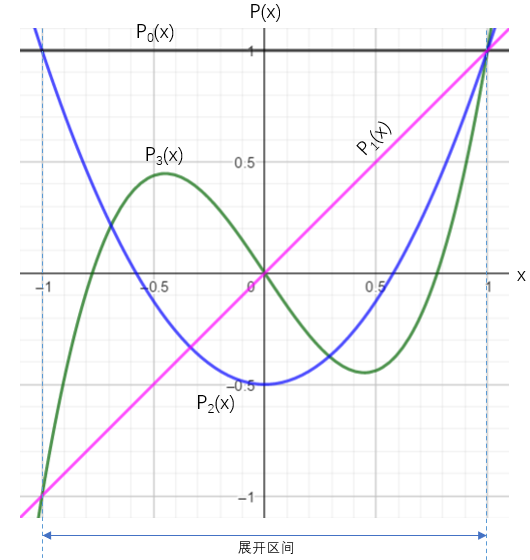
\includegraphics[scale=0.4]{./fig/2-6.png}
    \caption{勒让德多项式$P_n(x) \, , \, n=0,1,2,3$}
\end{figure}

因为$t$的幂是线性无关的,故可令等式两端$t^n$的系数相等:
\[xP_n-P_{n-1}=(n+1)P_{n+1}-2nxP_n+(n-1)P_{n-1}\]
\[(n+1)P_{n+1}-(2n+1)xP_n+nP_{n-1}=0 \tag{2-105}\]
它可将各种勒让德多项式联系起来。例如,给出$P_1$和$P_2$,就可小方程2-105中$n=2$求$P+3$:
\[P_3=\frac{(2 \cdot 1+1)xP_2-2P_1}{2+1}=\frac{5xP_2-2P_1}{3}=\frac{5x\left(\frac{3}{2}x^2-\frac{1}{2}\right)-2x}{3}=\frac{5}{2}x^3-\frac{3}{2}x \tag{2-106}\]
此递推关系式可用来造高次勒让德多项式。

方程2-87对$x$微商,可得另一关系式,
\[\frac{\partial F(x,t)}{\partial x}=\frac{t}{(1-2xt+t^2)^{\frac{3}{2}}}=\sum_nP'_n(x)t^n \tag{2-107}\]
由此式可将
\[t\sum_nP_n(x)t^n=(1-2xt+t^2)\sum_nP'_n(x)t^n \tag{2-108}\]
或,对$t^n$的系数,
\[P_{n-1}=P'_n-2xP'_{n-1}+P'_{n+1} \tag{2-109}\]
此递推关系式将勒让德多项式和它的一一阶导数联系起来。对母函数做类似的处理可以导出许多有用的关系式。

球谐函数:两个变量的正交归一函数组。勒让德微分方程(方程2-83)是下列方程的特例:
\[\dv{x}\left[(1+x^2)\dv{f}{x}\right]+\left[l(l+1)-\frac{m^2}{1-x^2}\right]f=0 \tag{2-110}\]
式中m是整数。若$m=0$,则方程2-110与2-83相同。此方程的解称为联属勒让德函数,
\[P_l^m(x)=(-1)^m(1-x^2)^{\frac{m}{2}}\dv[m]{P_l(x)}{x}\]
联属勒让德函数是由两个指标$m$和$l$标记。联属勒让德函数在区间$[-1,1]$也是正交的$\bra*{P_{l'}^m}\ket*{P_{l}^m}=0$。$l$不同和$m$相同的二联属勒让德函数的内积为零。联属勒让德函数的范数是
\[N(P_l^m)=\frac{2(l+m)!}{(2l+1)(l-m)!}\]
对确定的$m$和$l=m,m+1 \cdots $并定义在$[-1,1]$区间的函数组
\[\left \{\sqrt{\frac{(2l+1)(l-m)!}{2(l+m)!}}P_l^m(x) \right \}\]
是完备的和正交归-的。勒让德多项式是这组函数的特例,因为若$m=0$,这组函数与用施密特正交化造的函数组相同。

用$\cos \theta$代换x,联属勒让德函数可改写为在区间$0≤\theta≤\pi$的角变量$0$的函数。
因此,函数组$\{P_l^m(0)\}$是在$[0,π]$变 量为$θ$的完备的正交函数组。
在2-3节已见到$\{\frac{1}{\sqrt{2\pi}}e^{im\phi}\}$是在$[0,2\pi]$变量为$φ$的完备的正交归一函数组。
函数组$\{\sqrt{(2l+1)(l-m)!/2(l+m)!}P_l^m(\cos \theta)\}$的每一成员乘以完备正交归一函数组
$\{\frac{1}{\sqrt{2\pi}}e^{im\phi}\}$的每一成员,得到的函数组对二变量都是完备的和正交归一的,称为球谐函数:
\[Y_{l,m}(\theta,\phi)=\sqrt{\frac{(2l+1)(l-m)!}{4\pi(l+m)!}}P_l^m(\cos \theta)e^{im\phi} \tag{2-111}\]
同时
\[Y_{l,m}(\theta,\phi)=(-1)^mY_{l,m}^* \tag{2-112}\]
通常称指标m为球谐函数的“阶”,指标I为球谐函数的“次”。次
l取值$l=0,1,2 \cdots$;阶取值$-l,(-l+1),\cdots ,0, \cdots (l-1),l$。
\subsection*{总结}
现在用一些时间讨论勒让德多项式和联属勒让德多项式的内含和外延。
为了不使同学们见树不见林,我们现在扼要复述已讨论的问题的要点。

1.用施密特正交化,可由在$[-1,1]$的完备函数组$\{x^n\}$造出一组多项式。它就是没有归一化因子的勒让德多项式。

2.这些多项式是微分方程
\[\dv{x}\left[(1-x^2)\dv{f}{x}\right]+l(l+1)f=0\]
的解。

3.这些多项式是
\[F(x,t)=\frac{1}{\sqrt{1-2xt+t^2}}\]
以t的幂级数展开的系数。

4.这些多项式可从
\[P_l(x)=\frac{1}{2^ll!}\dv[l]{x}(x^2-1)^l\]
得出。

5.从3和4可导出许多关系式。

6.称做联属勒让德函数的
\[P_l^m(x)=(-1)^m(1-x^2)^{\frac{m}{2}}\dv[m]{P_l(x)}{x}\]
是微分方程
\[\dv{x}\left[(1-x^2)\dv{f}{x}\right]+l(l+1)f=0\]
的解。对不同的$l$和相同的$m$这些函数是正交的。

7.用归一化的调和函数$\{\frac{1}{\sqrt{2\pi}}e^{im\phi}\}$乘归一化的联属勒让德函数最形成的两个变量(角$\theta$和$\phi$)$Y_{l,m}(\theta,\phi)$在$0 \leq \theta \leq \pi$和$0≤\phi≤2\pi$是正交归一的和完备的。

本节试图说明下列两个想法:

1.讲清形成数学物理中重要特殊函数的几种方法。正交化,微分方程的幂级数解,和母函数。

2.为同学提供使用有关在化学中出现的一些函数的某些重要性质的资料(不需记忆)。
这些函数的行为,即便是定性描述,也能为化学体系提供有用的信息。
例如,因$P_{2l+1}(0)=0$,所以p和f原子轨道在垂直于轴的方向电子云密度为零。
同学们应像熟悉正弦函数和余弦函数那样努力掌握勒让德(及其它)函数,因而对用这些函数描述的化学体系的行为能够很容易地想象出来。

本节的大部分内容在别处都能找到。希望有些同学能够欣赏一下数学技巧,考察一下积分和导数的性质——但通常这对处理物理问题并不是最重要的部分。

本节以用于量子化学中的特殊函数的一览表做为总结。
\vspace{0.5cm}
\begin{center}
    \textbf{\Large{量子化学的特殊函数}}
\end{center}

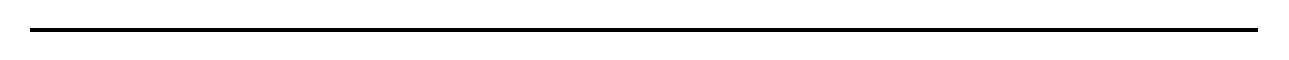
\begin{tikzpicture}
    \draw[ultra thick] (0,0) -- (15.6,0);
\end{tikzpicture}

\textbf{调和函数},$\{e^{imx}\}$

微分方程:
\[\dv[2]{f}{x}+m^2f=0\]

正交化:在$[0,2π]$区间

归一化因子:
\[\frac{1}{\sqrt{2\pi}}\]

存在:移动

\textbf{勒让德函数},$\{P(x)\}$

微分方程:
\[\dv{x}\left[(1-x^2)\dv{f}{x}\right]+l(l+1)f=0\]

正交化:对$[-1,1]$区间的$\{x^n\}$

归一化因子:
\[\sqrt{\frac{2l+1}{2}}\]

母函数:
\[\frac{1}{\sqrt{1-2xt+t^2}}=\sum_nP_n(x)t^n\]

存在:角运动。

联属勒让德函数,$\{P_l^m(x)\}$

微分方程:
\[\dv{x}\left[(1+x^2)\dv{f}{x}\right]+\left[l(l+1)-\frac{m^2}{1-x^2}\right]f=0\]

正交化:相同$m$,不同$l$,在区间$[-1,1]$

归一化因子:
\[\sqrt{\frac{(2l+1)(l-m)!}{2(l+m)!}}\]

存在:角运动

\textbf{拉基尔函数},$\{L_n(x)\}$

微分方程:
\[x\dv[2]{f}{x}+\dv{f}{x}-\left(\frac{1}{2}+\frac{x}{4}+n\right)f=0\]

正交化:对$[0,+\infty]$区间的$\{e^{-\frac{x}{2}}x^n\}$

归一化因子:
\[\frac{1}{n!}\]

母函数:
\[\frac{1}{1-t}e^{-\frac{xt}{1-t}}=\sum_nL_n(x)t^n\]

存在:径向运动

\textbf{厄米函数},$\{H_n(x)\}$

微分方程:
\[\dv[2]{f}{x}-2x\dv{f}{x}+2nf=0\]

正交化:对$(-\infty,+\infty)$区间的$\{e^{-\frac{x^2}{2}}x^n\}$

归一化因子:
\[\left(\frac{1}{\pi}\right)^{\frac{1}{4}}\frac{1}{\sqrt{2^nn!}}\]

母函数:
\[e^{2xt-t^2}=\frac{1}{n!}\sum_nH_n(x)t^n\]

存在:谐振子

\begin{problemset}
    \item 证明函数组$\{\sin mx,\cos nx\}$在m和n是正整数时在区间$[-\pi,\pi]$正交。
    \item 将下列函数按偶,奇,或非偶非奇分类,若函数既非偶又非奇,则将以函教分解成偶函数和奇函数之和。
    \[(a) \ x^2; \ (b) \ x^3; \ (c) \ x\sin x; \ (d) \ x^3\cos nx(n \in \mathbb{N_+}); \ (e) \ x^4; \ (f) \ \ln\left(\frac{1+x}{1-x}\right); \ (g) \ e^x; \ (h) \ e^{ix}\]
    \item 证明函数组$\{\sin mx\}$,$\{\cos nx\}$在区间$[0,\pi]$正交。求这些函数在区间的范数。计算用这些函数组展开的展开系数。
    \item 将函数$x-x^2$在区间$[-\pi,\pi]$\footnote{应该是$[0,\pi]$}展开,在区间$[0,\pi]$展成正弦级数,在区间$[0,\pi]$展成余弦级数。哪个展开式在$[0,\pi]$区间收敛的最快?
    \item 将函数$\sin^2x$在区间$[0,\pi]$展成正弦级数和余弦级数。哪个展开式收敛的最快?将结果与题4比较。
    \item 应用题4和题5的结果以及展开定理,计算在$[0,π]$的内积$\bra*{\sin x}\ket*{x-x^2}$。
    \item 证明函数组$\{e^{imx}\}$在区间$[0,2π]$正交。求此函数组的范数。计算用此函数组展开的展开系数。将这些系数与通常用富里叶级数展开的展开系数比较。
    \item “方波"是用在$0<x<\pi:f(x)=a,-\pi<x<0:f(x)=-a$定义的。对方波作富里叶级数展开。
    \item “三角波”是用在$-π≤x≤0:f(x)=x+π,0≤x≤π:f(x)=π-x$定义的。对三角波作富里叶级数展开。
    \item 证明函数组$\{exp(\frac{2ni\pi x}{b-a})\}$在区间$[a,b]$正交。
    \item 在零附近的泰勒级数是$x$的幂的展开式。泰勒级数是用正交函数展开的吗?证明各种正交归一函数组如何由用于泰勒级数的$x$的幂函数造出来的。
    \item 函数组$\{\sin^nx\}(n=0,1,2,\cdots)$不是正交归一函数组。 证明在$[-\pi,\pi]$用这组函数造的正交归一函数组就是题1的函数组。
    \item 用微分方程(方程2-110)证明联属勒让德函数事实上正如所述是正交的。
    \item 验证拉基尔多项式的正交化正如特殊函数表所列;验证其归一化因子。
    \item 验证厄米多项式的归一化因子正如特殊函数表所列。
    \item 将函数$e^x$展成勒让德多项式,厄米多项式和拉基尔多项式,井比较其结果。注意它们的展开区间十分不同。
    \item 对施密特正交化的讨论因展开区间的选择而有所不同。用一些尝试性例子说明改变展开区间对正交函数的影响是什么。
    \item 在光谱学中“选择定则”规定了哪些能级间的跃迁是允许的。对于
    “电偶级跃迁”光谱吸收的强度与称为跃迁偶级矩$\abs*{\bra*{\Psi_1}x\ket*{\Psi_2}}^2$成比例。
    计算谐振子的下列跃迁的跃迁偶极矩$(\Psi_n(x)=e^{-\frac{x^2}{2}}H_n(x))$,
    \[
    \begin{array}{ll}
        \Psi_1 \rightarrow \Psi_2 & \Psi_2 \rightarrow \Psi_3 \\
        \Psi_1 \rightarrow \Psi_3 & \Psi_2 \rightarrow \Psi_4 \\
        \Psi_1 \rightarrow \Psi_4
    \end{array}    
    \]
    你是否见到有什么花样出现?你能否列出并证明谐振子的一般选择定则?
\end{problemset}
\chapter{线性代数}
我们在第一章里简要地提到,量子力学可用两种观点处理。
第一,薛定谔波动力学将本征值方程表示为一个或多个变量函数的微分方程形式。
为了建立讨论薛定谔波函数所需的那种语言,在第二章里我们深入地研究了正交函数概念。
我们用解这样的微分方程(勒让德微分方程),并将其解与已建立的正交归一函数概念和性质联系起来做为总结。

研究量子力学的第二种观点是海森堡矩阵力学。本章将要建立研究矩阵力学的代数词汇。
也要以较完整的方式介绍在第一章里已提到的算符,导出量子化学中某些传统的有趣和重要结果。

\section{绪言}
我们就开始介绍一连串定义。
\begin{definition}[n维向量]
    一$n$维向量是$n$个数排成的数组:$\alpha=(\alpha_1,\alpha_2, \cdots ,\alpha_n)$。这n个数$\alpha_1,\alpha_2, \cdots ,\alpha_n$叫做向量的分量;它们是按规定的顺序排列;它们可为实数或虚数。
 \end{definition}

我们用希腊字母表示向量。三维空间中习用的物理向量就是一例,它的$x,y,z$分量分别用三个数表示。
\begin{definition}[向量空间]
    定义向量空间是具有下列二性质的向量的集合:
    
    (a) 定义唯一可对易的向量和为$\alpha^1+\alpha^2=\alpha^2+\alpha^1=(\alpha^1_1+\alpha^2_1,\alpha^1_2+\alpha^2_2,\cdots,\alpha^1_n+\alpha^2_n)$。
    
    (b) 定义任一向量$\alpha$和任一标量$c$的唯一积为$c\alpha=(c\alpha_1,c\alpha_2,\cdots,\alpha+n$,它既遵守分配律[即$c(\alpha+\beta)=c\alpha+c\beta$]又遵守结合律[即$(c_1c_2)\alpha=c_1(c_2\alpha)$]。    
\end{definition}

同学们应了解三维物理向量的这些性质。我们用上标表示向量组的成员${\alpha^i}$,用下标表示单个向量的分量。
\begin{definition}[欧氏向量空间]
    欧氏向量空间是这样的向量空间,其向量的分量是实数的,且任二向量的内积$\bra*{\alpha}\ket*{\beta}=\alpha_1\beta_1+\alpha_2\beta_2+\cdots+\alpha_n\beta_n$是实数的,
    它是对称的[$\bra*{\alpha}\ket*{\beta}=\bra*{\beta}\ket*{\alpha}$],双线性的[$\bra*{\alpha+\beta}\ket*{\gamma}=\bra*{\alpha}\ket*{\gamma}+\bra*{\beta}\ket*{\gamma}$]
    \footnote{关于双线性的定义应该是$\bra*{c_1\alpha^1+c_2\alpha^2}\ket*{\beta}=c_1\bra*{\alpha^1}\ket*{\beta}+c_2\bra*{\alpha^2}\ket*{\beta},\bra*{\alpha}\ket*{c_1\beta^1+c_2\beta^2}=c_1\bra*{\alpha}\ket*{\beta^1}+c_2\bra*{\alpha}\ket*{\beta^2}$,下一个定义中的双线性也相同。},和正值的[$\bra*{\alpha}\ket*{\alpha} \geq 0$]。
\end{definition}

此内积定义用的符号$\bra*{}\ket*{}$就是函数内积用的符号。

在稍微不同和更一般化的向量空间定义中,内积的定义也稍微不同和更一般化。
\begin{definition}[厄米向量空间]
    厄米向量空间是这样的向量空间, 其向量的分量可为复数,且任二向量可有复数内积$\bra*{\alpha}\ket*{\beta}=\alpha_1^*\beta_1+\alpha_2^*\beta_2+\cdots+\alpha_n^*\beta_n$,
    它是厄米的[$\bra*{\alpha}\ket*{\beta}=\bra*{\beta}\ket*{\alpha}^*$],双线性的[$\bra*{\alpha+\beta}\ket*{\gamma}=\bra*{\alpha}\ket*{\gamma}+\bra*{\beta}\ket*{\gamma}$],和正值的[$\bra*{\alpha}\ket*{\alpha} \geq 0$]。    
\end{definition}

应做两个比较。首先,比较这里的内积定义
\[\bra*{\alpha}\ket*{\beta}=\sum_i\alpha^*_i\beta_i \tag{3-1}\]
和第二章里内积的定义(方程2-1)
\[\bra*{f}\ket*{g}=\int f^*(x)g(x)\dd{x}\]
其差别在于向量内积定义是对不连续指标求和,而函数内积则是对连续变量积分。
此差别(不连续指标替换连续变量)在辨别海森堡和薛定谔图象时更明显。

另外,应看到欧氏向量空间和厄米向量空间的区别:欧氏向量空间中内积是实的和对称的;厄米向量空间中内积是复的和厄米的。
应将厄米向量空间中内积的这个性质和二函数内积的类似性质忆比:内积换位给出该内积的复共轭。
\begin{definition}[向量正交]
    若二向量的内积为零,则此二向量正交。
\end{definition}

此定义与函数正交性的定义是严格平行的;这使正交性成为一个更广义的概念,并与垂直向量这一为人们熟悉的性质建立联系。
\begin{definition}[向量范数]
    同样与已讲过的函数的有关内容类比,向量的范数定义为:$N(\alpha)=\bra*{\alpha}\ket*{\alpha}=\abs*{\alpha}^2$。
\end{definition}

范数对应于三维物理向量空间中向量的长度。最后的两个定义继续表明向量空间代数与函数微积分的平行结构。

\begin{definition}[向量归一化,正交归一向量组]
    若一向量的范数为一,则称该向量是归一化的。
    
    若向量组中每一向量是归一化的,且任一向量与任一其它向量都正交,则该向量组是正交归一向量组。
\end{definition}

我们用证明施瓦兹不等式做为对这些定义的说明。

\begin{theorem}[施瓦兹不等式]
    \[\abs*{\bra*{\alpha}\ket*{\alpha}} \leq \abs*{\alpha} \cdot \abs*{\beta}\]
\end{theorem}

若$\alpha$或$\beta$为零,则为等号,但定理没有意义。若$\alpha$和$\beta$都不为零,则可借二任意标量$c$和$d$之助构成此定理。根据内积的正值性,
\[0 \leq \bra*{c\alpha+d\beta}\ket*{c\alpha+d\beta} \tag{3-2}\]
和内积的双线性关系
\[0 \leq c^*\bra*{\alpha}\ket*{c\alpha+d\beta}+d^*\bra*{\beta}\ket*{c\alpha+d\beta}\]
\[\leq c^*c\bra*{\alpha}\ket*{\alpha}+c^*d\bra*{\alpha}\ket*{\beta}+d^*c\bra*{\beta}\ket*{\alpha}+d^*d\bra*{\beta}\ket*{\beta} \tag{3-3}\]
c和d为任何值方程都成立;因此,对特定值$c=-\bra*{\alpha}\ket*{\beta}$和$d=\bra*{\alpha}\ket*{\alpha}$方程也应成立。将这些值代入方程3-3,得出
\[0 \leq c^*cd-c^*dc-d^*cc^*+d^*d\bra*{\beta}\ket*{\beta}=d^*[-cc^*+d\bra*{\beta}\ket*{\beta}] \tag{3-4}\]
因此,
\[0 \leq -\abs*{\bra*{\alpha}\ket*{\beta}}^2+\bra*{\alpha}\ket*{\alpha}\bra*{\beta}\ket*{\beta} \tag{3-5}\]
或
\[\abs*{\bra*{\alpha}\ket*{\beta}}^2 \leq \abs*{\alpha}^2\abs*{\beta}^2 \tag{3-6}\]
\[\abs*{\bra*{\alpha}\ket*{\beta}} \leq \abs*{\alpha}\abs*{\beta} \tag{3-7}\]

建立了对函数和向量都能应用的内积和范数的定义后,我们就可以将对函数已深入研究过的那些结果应用于向量。
先考虑向量组;其结果在很大程度上与早先研究函数组的结果平行。

向量空间有与函数组完备性类似的概念。
\begin{definition}[向量空间]
    若向量空间的任一向量都能用向量组$\{\alpha^i\}$的线性组合表示,则该向量空间为向量组$\{\alpha^i\}$张成(Span)。
\end{definition}

通常的三维欧氏向量空间(以后称之为3D空间)能够很容易地将此定义用图表示出来。
例如,向量$(1,0,0),(0,1,0),(0,0,1)$张成3D空间。
这些向量正是三个坐标方向上的单位向量,任何向量可用三单位向量的线性组合表示,这是大家熟悉的事实。
这个定义促使我们对维的概念做更严格的解释。

\begin{definition}[向量空间的维数]
    向量空间的维是张成该向量空间所需的向量的最小数目。
\end{definition}

在上例中任二向量都不足以张成3D空间,但四个向量,如$(1,0,0),(0,1,0),(0,0,1),(1,1,1)$,又是多余的。
向量组$(1,0,0),(0,1,0),(1,1,0)$虽然数目是三,但不能张成3D空间。
希望读者能看出为什么。这些向量不是线性无关的,因而有一个是多余的。这样,线性无关的概念又在讨论向量空间时出现。

\begin{definition}[线性相关,线性无关]
    若只有全部$c_i=0$时方程
    \[c_1\alpha^1+c_2\alpha^2+\cdots+c_n\alpha^n=\sum_ic_i\alpha^i=0 \tag{3-8}\]
    才可解,则向量组$c_1 ,c_2,\cdots,c_n$是线性无关的。若方程3-8在某些$c_i \neq 0$时可解,则向量组$\{\alpha^i\}$是线性相关的。
\end{definition}

向量空间的这些性质使我们得出基这一方便概念。

\begin{definition}[基,正交归一基]
    向量空间的基是可张成向量空间的某些线性无关的向量组;
    
    向量空间的正交归一基是可张成该空间的某些正交归一向量组。
\end{definition}

可将此定义与由线性无关函数组造正交归一函数组的过程(施密特正交化)联系起来。施密特正交化可不加修正地用于向量。
若用$\{\alpha^i\}$表示线性无关向量组,$\{\phi^i\}$表示正交归一向量组,则可得有关公式如下:
\[\phi^k=\frac{1}{\sqrt{N_k}}(\alpha^k-\sum_{j=0}^{k-1}\bra*{\phi^j}\ket*{\phi^k}\phi^j) \tag{3-9}\]
\[N_k=\bra*{\alpha^k}\ket*{\alpha^k}-\sum_{j=0}^{k-1}\abs*{\bra*{\phi^j}\ket*{\phi^k}}^2 \tag{3-10}\]

由于向量几乎在所有方面都与正交归一函数平行,无疑全部代数“机器”都可用于将向量展成正交归一向量组。
在第二章中放在一起的那组方程(方程2-19——2-24) 可精确地用于向量问题。
因此,可按下列公式将任一向量$\xi$展成向量组$\{\phi^i\}$
\[\xi=\sum_ic_i\phi^i \tag{3-11}\]
其展开系数(可能是复数)为
\[c_i=-\bra*{\phi^i}\ket*{\xi} \tag{3-12}\]

也可从第二章将内积的展开定理借来用,
\[\bra*{\xi}\ket*{\eta}=\sum_i\bra*{\xi}\ket*{\phi^i}\bra*{\phi^i}\ket*{\eta} \tag{3-13}\]
式中$\{\phi^i\}$是正交归一向量组。

离开平行研究向量空间和函数,讨论一有用问题 ,这就是对有限维向量空间直接检验向量组是否线性无关。
读者可能还记得,在讨论函数组时曾暂时离开主题谈到此问题,并且更多地依赖直觉而非严格推理。

然而,对向量组我们可以仔细地作分析以确定向量组(有限的)是否线性无关。
由于出现了称为矩阵的数学元素,故此分析既为本节作出适合的总结,又是下节的导言。
在考虑线性无关时,我们尝试求符合方程3-8而又不为零的$c_i$。为了使求法比尝试法好些,提出一简单步骤。

将向量排成行。设有三个向量$\alpha,\beta,\gamma$每个向量有四个分量。其排列的形状如下:
\[
\begin{array}{cccc}
    \alpha_1 & \alpha_2 & \alpha_2 & \alpha_2 \\
    \beta_1 & \beta_2 & \beta_3 & \beta_4 \\
    \gamma_1 & \gamma_2 & \gamma_3 & \gamma_4
\end{array}    
\]
从底行作起。一定能找到一倍数乘$\alpha_1$加$\gamma_1$等于零。事实上此倍数就是$-\frac{\gamma_1}{\alpha_1}$。
将第一行所有$\alpha_1$;都乘此常数并加到底行上。现在排列的形状如下:
\[
\begin{array}{llll}
    \alpha_1 & \alpha_2 & \alpha_2 & \alpha_2 \\
    \beta_1 & \beta_2 & \beta_3 & \beta_4 \\
    0 & \gamma_2-\frac{\gamma_1}{\alpha_1}\alpha_2 & \gamma_3-\frac{\gamma_1}{\alpha_1}\alpha_3 & \gamma_4-\frac{\gamma_1}{\alpha_1}\alpha_4
\end{array}    
\]
用同样方法可以“消去”$\beta_1$,即找出一倍数乘$\alpha_1$加$\beta_1$:等于零。继续进行下去(下一步是消去$\gamma_2$),可得出下边那样排列:
\[
\begin{array}{llll}
    \times & \times & \times & \times \\
    0 & \times & \times & \times \\
    0 & 0 & \times & \times
\end{array}    
\]
像这样没有一行全为零,而左下角全为零的排列表明$\alpha,\beta,\gamma$线性组合都不为零,因而这些向量是线性无关的。若排列形状如下:
\[
\begin{array}{llll}
    \times & \times & \times & \times \\
    0 & \times & \times & \times \\
    0 & 0 & 0 & 0
\end{array}    
\]
则有$\alpha,\beta,\gamma$的某些线性组合为零(底行),因而这些向量是线性相关的。

现在可将这种想法归纳成文。

\begin{definition}
    \textbf{矩阵} \quad 标量(实数或复数)的矩形排列叫做矩阵。位于第$i$行第$j$列的标量称为矩阵的$i,j$矩阵元。$n$行$m$列的矩阵记为$n \times m$矩阵。

    \textbf{矩阵初等运算} \quad 对矩阵实施的初等行运算为:

    1.用常数乘行。
    
    2.两行相加。
    
    3.交换两行。

    \textbf{对角元} \quad 矩阵A的对角线(或主对角线)上的矩阵元为$\{a_{ii}\}$,即$a_{11},a_{22},a_{33},\cdots$等等。这些矩阵元称为对角元。
    
    \textbf{三角矩阵} \quad 若一矩阵其对角左下方的矩阵元皆为零,则该矩阵称为三角矩阵。\footnote{这里更应该叫上三角矩阵。}

    \textbf{行等价} \quad 用初等行运算可彼此形成的矩阵称为行等价。

    \textbf{向量组的线性无关} \quad 若以向量的分量为行形成的矩阵是非\footnote{这里译作“无”更好。}全为零的行的三角矩阵的行等价矩阵,则此向量组是线性无关的。
\end{definition}

此定理表示\footnote{奇怪的表述方式,感觉“揭示”更好。}出我们提出的检验线性无关的方法。用二例说明该定理和方法。

\textbf{例1}

向量$(1,-1,3),(2,-4,1)(0,3,2)$线性无关吗?先形成矩阵(放在括号里),再进行初等行运算。
(3,1)矩阵元已经是零。-2乘第一行加到第二行上使(2,1)矩阵元为零。为了简化,用$-\frac{1}{2}$乘第二行。
-3乘第二行加到第三行,上使(3,2)矩阵元为零。现在矩阵成三角形。所有行都至少含一不为零的矩阵元;因此,这些向量是线性无关的。

\[
\begin{pmatrix}
    1 & -1 & 3 \\
    2 & -4 & 1 \\
    0 & 3 & 2
\end{pmatrix}    
\xrightarrow{r_2-2r_1}
\begin{pmatrix}
    1 & -1 & 3 \\
    0 & -2 & -5 \\
    0 & 3 & 2
\end{pmatrix} 
\xrightarrow{-\frac{1}{2} \cdot r_2}
\begin{pmatrix}
    1 & -1 & 3 \\
    0 & 1 & \frac{5}{2} \\
    0 & 3 & 2
\end{pmatrix} 
\xrightarrow{r_3-3r_2}
\begin{pmatrix}
    1 & -1 & 3 \\
    0 & 1 & \frac{5}{2} \\
    0 & 0 & -\frac{11}{2}
\end{pmatrix} 
\]

\textbf{例2}

向量$(1,2i,1+i),(4,6-i,7),(-2,-6+5i,-5+2i)$线性无关吗?
还是先形成矩阵,再系统地实 施初等行运算。
\[
\begin{pmatrix}
    1 & 2i & 1+i \\
    4 & 6-i & 7 \\
    -2 & -6+5i & -5+2i
\end{pmatrix}    
\xrightarrow{r_3+2r_1}
\begin{pmatrix}
    1 & 2i & 1+i \\
    4 & 6-i & 7 \\
    0 & -6+9i & -3+4i
\end{pmatrix}    
\xrightarrow{r_2-3r_1}
\begin{pmatrix}
    1 & 2i & 1+i \\
    0 & 6-9i & 3-4i \\
    0 & -6+9i & -3+4i
\end{pmatrix}
\]
\[
\xrightarrow{r_3+r_2}
\begin{pmatrix}
    1 & 2i & 1+i \\
    0 & 6-9i & 3-4i \\
    0 & 0 & 0
\end{pmatrix}
\]

矩阵成三角形。有一行全为零;因此,这些向量线性相关。我们能够返回来作并求出满足方程3-8的常数:
\[2\alpha^1+\alpha^3+(-4\alpha^1+\alpha^2)=0\]
\[-2\alpha^1+\alpha^2+\alpha^3=0\]

本节用与函数对比的方法导出向量的-些性质。施密特正交化,展成正交归-基组,展开定理都是从第二章借来的结果。
介绍了检验线性无关的简易方法。在此检验方法中引入称为矩阵的代数元素,以及它的某些性质和成分,诸如矩阵元,对角元,行和列,行等价。

\section{矩阵、行列式和线性方程组}
矩阵。在上节中矩阵的定义是做为检验向量的线性无关的形式辅助手段而引入的。而矩阵有比做为这种问题的辅助手段更多的用途。
从量子力学的观点看,如第一章已提出的那样,矩阵可用来表示算符。矩阵的这个用途将在本章第四节详细讨论,它也促使我们现在要讨论更多的矩阵性质。

\begin{definition}[矩阵加法]
    二矩阵只有维数相同才能相加。$n \times m$矩阵A与$n \times m$矩阵B的和是$n \times m$矩阵C,其矩阵元由下列给出:
    \[c_{ij}=a_{ij}+b_{ij} \tag{3-14}\]
\end{definition}

也就是说,矩阵相加就是它们的矩阵元相加。我们用大写字母记矩阵,小写字母记它们的矩阵元。

\textbf{例}
\[
\begin{pmatrix}
    1 & 3 & 2 & 5 \\
    0 & 7 & 9 & 4 \\
    6 & -2 & 5 & 1 
\end{pmatrix}    
+
\begin{pmatrix}
    4 & -3 & 1 & -6 \\
    0 & 0 & -2 & 1 \\
    1 & -1 & 1 & -1 
\end{pmatrix}
=
\begin{pmatrix}
    5 & 0 & 3 & -1 \\
    0 & 7 & 7 & 5 \\
    7 & -3 & 6 & 0 
\end{pmatrix}   
\]

相加的定义不会使同学们惊异,而相乘的定义却与二数相显的通常概念不同。

\begin{definition}[矩阵乘法]
    只有乘数矩阵的列与被乘矩阵的行相同时,二矩阵才可相乘。$n \times m$矩阵4与$m \times p$矩阵B相乘得出$n \times p$矩阵C,其矩阵元由下式给出:
    \[c_{ij}=\sum_{k=1}^ma_{ik}b_{kj} \tag{3-15}\]
\end{definition}

应注意二矩阵可相乘的条件。
\[(n \times m)(m \times p)=(n \times p)\]
维数相同的方阵永远可乘,这是特殊情况\footnote{原书这里笔误写成$(n \times m)(n \times n)=(n \times n)$。}。
\[(n \times n)(n \times n)=(n \times n)\]
因为我们将要用方阵表示算符,所以方阵的性质对我们特别重要。

对二矩阵如何相加和如何相乘作一比较。矩阵相加是它们的矩阵元相加,但矩阵相乘却不是矩阵元简单地相乘。
虽然在许多情况下可就事论事地使用方程3-15,但从实际运算中了解方程的含义是有益的。
假设我们希望计算$2 \times 3$矩阵和$3 \times 4$矩阵的积。结果是$2 \times 4$矩阵,其(2,3)矩阵元由下式给出:
\[c_{23}=\sum_{k=1}^3a_{2k}b_{k3}=a_{21}b_{13}+a_{22}b_{23}+a_{23}b_{33} \tag{2-16}\]
图解有助于将参加运算的那些矩阵元显示出来。

人们(即便是专业人员)在乘矩阵时常常将左食指点在被乘矩阵(左)的行上,右食指放在乘数矩阵(右)的列上。

\begin{figure}[htbp]
    \centering
    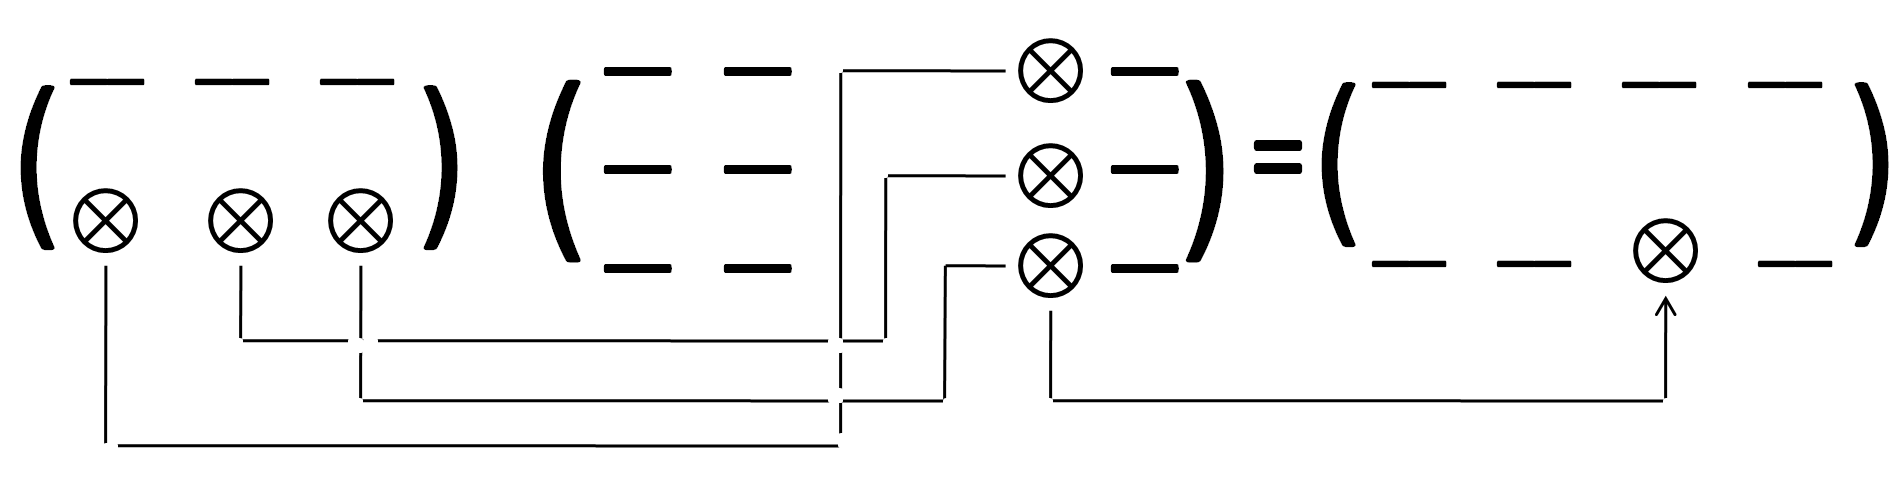
\includegraphics[scale=0.22]{./fig/3-0.png}
\end{figure}

\textbf{例1}

求下边矩阵的积。
\[
\begin{pmatrix}
    3 & 1 & 2 \\
    1 & 2 & 3
\end{pmatrix}
\begin{pmatrix}
    1 & 0 & 1 & 0 \\
    0 & 1 & 0 & 1 \\
    1 & 0 & 1 & 0
\end{pmatrix}    
=
\begin{pmatrix}
    C_{11} & C_{12} & C_{13} & C_{14} \\
    C_{21} & C_{22} & C_{23} & C_{24}
\end{pmatrix} 
\]
用方程3-15计算这八个矩阵元:
\[
\begin{array}{ll}
    C_{11}=3 \cdot 1+1 \cdot 0+2 \cdot 1=5 & C_{21}=1 \cdot 1+2 \cdot 0+3 \cdot 1=4 \\
    C_{11}=3 \cdot 0+1 \cdot 1+2 \cdot 0=1 & C_{21}=1 \cdot 0+2 \cdot 1+3 \cdot 0=2 \\
    C_{11}=3 \cdot 1+1 \cdot 0+2 \cdot 1=5 & C_{21}=1 \cdot 1+2 \cdot 0+3 \cdot 1=4 \\
    C_{11}=3 \cdot 0+1 \cdot 1+2 \cdot 0=1 & C_{21}=1 \cdot 0+2 \cdot 1+3 \cdot 0=2
\end{array}    
\]
其积为
\[
\begin{pmatrix}
    5 & 1 & 5 & 1  \\
    4 & 2 & 4 & 2
\end{pmatrix}    
\]
同学们应验证一下这些矩阵元,同时也可巩固乘二矩阵的“食指法”。

\vspace{0.5cm}

\textbf{例2}

求下列二方阵的积。
\[
\begin{pmatrix}
    1 & 2 \\
    3 & 4
\end{pmatrix}      
\begin{pmatrix}
    4 & 3 \\
    2 & 1
\end{pmatrix} 
=
\begin{pmatrix}
    8 & 5 \\
    20 & 13
\end{pmatrix}   
\]

矩阵相乘的另一特殊性质是不可对易性。标量相乘,标量和矩阵相加都是可对易的运算:$ab=ba,a+b=b+a,A+B=B+A$一般讲,矩阵相乘是不可对易的:$AB \neq BA$。
因为非方阵不能从个方向相乘,所以我们只考虑方阵的对易问题。在例2中,
\[
\begin{pmatrix}
    1 & 2 \\
    3 & 4
\end{pmatrix}      
\begin{pmatrix}
    4 & 3 \\
    2 & 1
\end{pmatrix} 
=
\begin{pmatrix}
    8 & 5 \\
    20 & 13
\end{pmatrix}   
\neq
\begin{pmatrix}
    13 & 20 \\
    5 & 8
\end{pmatrix}   
=   
\begin{pmatrix}
    4 & 3 \\
    2 & 1
\end{pmatrix} 
\begin{pmatrix}
    1 & 2 \\
    3 & 4
\end{pmatrix}   
\]

继续讨论矩阵的初等算术。下面介绍与数相似的两个矩阵。矩阵元全为零的矩阵叫做零矩阵,0。和数零相似,零知比加任何矩阵(同维)仍得该矩阵:
\[A+0=A \tag{3-17}\]

对角元全为一,非对角元全为零的矩阵(方阵)叫做恒等或单位矩阵,$E$(或记着$I$或$1$)。用克朗尼克符号可使此定义很简洁。我们义定
\[e_{ii}=1 \tag{3-18a}\]
对全部$i$,
\[e_{ij}=1 \tag{3-18a}\]
对全部$i \neq j$。这和定义
\[e_{ij}=\delta_{ij}\]
等价。只对方阵定义的恒等矩阵具有与数一相似的性质,即$E$与任何矩阵(方阵并与E同维)的积仍为该矩阵: $EA=A$。

做为使用一般化公式(方程3-15)的练习,我们证明$E$与所有矩阵都可对易。积$EA$的$ij$矩阵元是
\[(EA)_{ij}=\sum_ke_{ik}a_{kj}=\sum_k\delta_{ik}a_{kj}=a_{ij} \tag{3-19}\]
而
\[(AE)_{ij}=\sum_ka_{kj}e_{ik}=\sum_ka_{kj}\delta_{ik}=a_{ij}=(EA)_{ij} \tag{3-19}\]
既然有与数一的性质相似的矩阵,那么是否也有与倒数(因而与商)相似的矩阵?

\begin{definition}[逆矩阵]
    方阵$A$的逆矩阵(记着$A^{-1}$)是遵守下列关系的矩阵:
    \[A^{-1}A=AA^{-1}=E\]
    只对方阵定义逆矩阵。
\end{definition}

我们将讨论求逆矩阵的两个方法。第一个方法与上节介绍的检验线性无关的方法相似。第二个方法是用行列式定义的,我们稍后再讨论。行等价概念是找到第一个方法的线索。

\begin{theorem}[矩阵求逆]
    只有其行是线性无关的方阵$A$才有逆。可用下列步骤求逆。对$A$实施初等行运算使之变成$E$。然后以相同的顺序对$E$实施相同的行运算使之成$A^{-1}$。
\end{theorem}

应注意,一矩阵即便是非零矩阵也不定有逆。

正如上节的定理提示的那样,只有方阵$A$的行线性无关,$A$才是$E$的行等价矩阵。本定理的证明留给感兴趣的读者到许多好的代数教科书中去查找。我们只用一例来说明。

\textbf{例}

求下列方阵$A$的逆:
\[A=
\begin{pmatrix}
    1 & 2 \\
    3 & 4
\end{pmatrix} 
\]
先对$A$实施初等行运算使之成$E$:
\[
\begin{pmatrix}
    1 & 2 \\
    3 & 4
\end{pmatrix}    
\xrightarrow{r_2-3r_1}
\begin{pmatrix}
    1 & 2 \\
    0 & -2
\end{pmatrix} 
\xrightarrow{-\frac{1}{2} \cdot r_2}
\begin{pmatrix}
    1 & 2 \\
    0 & 1
\end{pmatrix} 
\xrightarrow{r_1-2r_2}
\begin{pmatrix}
    1 & 0 \\
    0 & 1
\end{pmatrix} 
=E
\]
然后对$E$实施相同运算:
\[
\begin{pmatrix}
    1 & 0 \\
    0 & 1
\end{pmatrix}
\xrightarrow{r_2-3r_1}
\begin{pmatrix}
    1 & 0 \\
    -3 & 1
\end{pmatrix}
\xrightarrow{-\frac{1}{2} \cdot r_2}
\begin{pmatrix}
    1 & 0 \\
    \frac{3}{2} & -\frac{1}{2}
\end{pmatrix}
\xrightarrow{r_1-2r_2}
\begin{pmatrix}
    -2 & 1 \\
    \frac{3}{2} & -\frac{1}{2}
\end{pmatrix}
=A^{-1}
\]
将答案乘以$A$以验证之:
\[
\begin{pmatrix}
    -2 & 1 \\
    \frac{3}{2} & -\frac{1}{2}
\end{pmatrix}   
\begin{pmatrix}
    1 & 2 \\
    3 & 4
\end{pmatrix} 
=
\begin{pmatrix}
    1 & 0 \\
    0 & 1
\end{pmatrix} 
\]
这种技巧既麻烦又易出错;同学们将会发现用行列式技巧比较保险。我们再用一个定义结束矩阵代数的讨论。

\begin{definition}[矩阵转置]
    方阵$A$的转置记为$A'$,其矩阵元
    \[a_{ij}'=a_{ji}\]
    以$A$的对角线为轴将矩阵翻转可得出$A'$。
\end{definition}

矩阵的转置在量子力学中很重要。转置的乘法遵守简单规则,
\[(AB)'=B'A' \tag{3-21}\]
若逆存在,它也遵守该规则,
\[(AB)^{-1}=B^{-1}A^{-1} \tag{3-22}\]

行列式。行列式的正式定义相当复杂,因此我们从使用行列式的实例开始。行列式的一个重要应用是解联立线性方程组。取下列方程组为例:
\[
\begin{array}{c}
    a_{11}x_1+a_{12}x_2=b_1 \\
    a_{21}x_1+a_{22}x_2=b_2
\end{array}    
\tag{3-23}
\]
将方程组写成这样形式就是要把我们引上以后要展开的矩阵观点。现在我们用代入法解方程3-23。
由第二个方程得$x_2=(b_2-a_{21}x_1)/a_{22}$,代入第一个方程,得出解
\[x_1=\frac{a_{22}b_1-a_{12}b_2}{a_{11}a_{22}-a_{12}a_{21}} \tag{3-24}\]
陈述式的分母包含联立方程组3-23的全部四个系数。事实上,分母就是称为系数矩阵的行列式。
\[A=
\begin{pmatrix}
    a_{11} & a_{12} \\
    a_{21} & a_{22} 
\end{pmatrix}
\tag{3-25a}
\]
\[
\begin{vmatrix}
    a_{11} & a_{12} \\
    a_{21} & a_{22} 
\end{vmatrix} 
\equiv
a_{11}a_{22}-a_{12}a_{21}
\tag{3-25b}
\]
方程3-24的分子也可写成行列式,因此结果为
\[
x_1=
\frac{
\begin{vmatrix}
    b_1 & a_{12} \\
    b_2 & a_{22} 
\end{vmatrix} 
}
{
\begin{vmatrix}
    a_{11} & a_{12} \\
    a_{21} & a_{22} 
\end{vmatrix} 
}   
\qquad 
x_2=
\frac{
\begin{vmatrix}
    a_{11} & b_1 \\
    a_{21} & b_2 
\end{vmatrix} 
}
{
\begin{vmatrix}
    a_{11} & a_{12} \\
    a_{21} & a_{22} 
\end{vmatrix} 
} 
\tag{3-26}
\]
此结果是以后要讨论的克拉姆规则的特例。方程3-25b给出$2 \times 2$行列式的简单定义。对应于大方阵的行列式的定义更复杂,不能从方程3-25b导出。
\begin{definition}[排列]
    $n$个整数的排列$P$是有序地排$n$个整数的一种方式;有$n!$个这样的排列。
    若排列中二指标换位数为偶;则P的符号为正;若排列中二指标换位数为奇,则$P$为负。
    \footnote{这里的二指标换位数定义应该与逆序数定义等价。}
\end{definition}
\textbf{例}

对整数$(1,2,3)$来讲,$(2,1,3)$是奇排列;$(2,3,1)$是偶排列。
\begin{definition}[行列式]
    方阵A的行列式记着$|A|$或$det \, A$;它是一个数(实数或复数),可用下式求出:
    \[|A|=\sum_{all \ P}^{n!}Sgn(P)a_{1,p_1}a_{2,p_2} \cdots a_{n,p_n} \tag{3-27}\]
\end{definition}
\textbf{例}

取$3 \times 3$行列式做为求行列式公式的例子。有$3!=6$项。求

\[
\begin{vmatrix}
    a_{11} & a_{12} & a_{13} \\
    a_{21} & a_{22} & a_{23} \\
    a_{31} & a_{32} & a_{33}
\end{vmatrix}    
\]
\[
\begin{tabular}{|c|c|c|c|}
    \hline
    项 & 排列 & 重排数 & Sgn(P) \\ \hline
    $a_{11} \ a_{22} \ a_{33}$ & 1 \ 2 \ 3 & 0 & + \\
    $a_{11} \ a_{23} \ a_{32}$ & 1 \ 3 \ 2 & 1 & - \\
    $a_{12} \ a_{21} \ a_{33}$ & 2 \ 1 \ 3 & 1 & - \\
    $a_{12} \ a_{23} \ a_{31}$ & 2 \ 3 \ 1 & 2 & + \\
    $a_{13} \ a_{22} \ a_{31}$ & 3 \ 2 \ 1 & 1 & - \\
    $a_{13} \ a_{21} \ a_{32}$ & 3 \ 1 \ 2 & 2 & + \\
    \hline
\end{tabular}
\]
以正确的符号\footnote{因个人技术能力有限,上表与原书有部分出入,基本想表达的思想应该是相同的。}将这些项加在一起,得出
\[|A|=a_{11}a_{22}a_{33}+a_{12}a_{23}a_{31}+a_{13}a_{21}a_{32}-a_{11}a_{23}a_{32}-a_{12}a_{21}a_{33}-a_{13}a_{22}a_{31} \tag{3-28}\]

这充其量也是一繁琐的步骤,但有比较简单的办法。将所有含$a_{11}$,$a_{12}$和$a_{13}$的项分别组合在一起,可得到简单办法的线索。
\[|A|=a_{11}(a_{22}a_{33}-a_{23}a_{32})+a_{12}(a_{23}a_{31}-a_{21}a_{33})+a_{13}(a_{21}a_{32}-a_{22}a_{31}) \tag{3-29a}\]
\[
=a_{11}
\begin{vmatrix}
    a_{22} & a_{23} \\
    a_{32} & a_{33}
\end{vmatrix}  
-a_{12}
\begin{vmatrix}
    a_{21} & a_{23} \\
    a_{31} & a_{33}
\end{vmatrix}  
+a_{13}
\begin{vmatrix}
    a_{21} & a_{22} \\
    a_{31} & a_{32}
\end{vmatrix}  
\]
方程3-29a表明行列式展成余因式;方程3-29b表明行列式展成余子式。

\begin{definition}[余因式,余子式]
    $n \times n$方阵的矩阵元$a_{ij}$的余因式$A_{ij}$是用$(n-1) \times (n-1)$行列式表示的数,余因式与行列式$|A|$的关系为
    \[|A|=\sum_ja_{ij}A_{ij} \tag{3-30}\]
    对任一i皆可。$n \times n$方阵的矩阵元$a_{ij}$的余子式$M_{ij}$是用$(n-1) \times (n-1)$行列式表示的数,此行列式是将$A$的$i$行和$j$列去掉而形成的。余子式和余因式最多差一符号:
    \[A_{ij}=M_{ij}(-1)^{i+j}\]
\end{definition}

\textbf{例}

取$4 \times 4$矩阵的$2,3$余子式和余因式为例,去掉第二行,去掉第三列。
\[
A=
\begin{pmatrix}
    a_{11} & a_{12} & a_{13} & a_{14} \\
    a_{21} & a_{22} & a_{23} & a_{24} \\
    a_{31} & a_{32} & a_{33} & a_{34} \\
    a_{41} & a_{42} & a_{43} & a_{44} 
\end{pmatrix}    
\]
\[
M_{23}=
\begin{vmatrix}
    a_{11} & a_{12} & a_{14} \\
    a_{31} & a_{32} & a_{34} \\
    a_{41} & a_{42} & a_{44} 
\end{vmatrix}    
\]
\[
A_{23}=-
\begin{vmatrix}
    a_{11} & a_{12} & a_{14} \\
    a_{31} & a_{32} & a_{34} \\
    a_{41} & a_{42} & a_{44} 
\end{vmatrix}    
=(-1)^{2+3}M_{23}
\]

\begin{theorem}
    $n \times n$矩阵$A$的行列式可展成余因式或余子式:
    \[|A|=\sum_ja_{ij}A_{ij}=\sum_ja_{ij}(-1)^{i+j}M_{ij}\]
    对任何$i$皆可。
\end{theorem}

\textbf{例}

用展成余子式和直接用方程3-28求下列$3 \times 3$行列式的值。
\[
\begin{vmatrix}
    1 & 0 & 2 \\
    3 & 4 & -1 \\
    -2 & 1 & 1
\end{vmatrix}    
=1
\begin{vmatrix}
    4 & -1 \\
    1 & 1
\end{vmatrix} 
-0
\begin{vmatrix}
    3 & -1 \\
    -2 & 1
\end{vmatrix} 
+2
\begin{vmatrix}
    4 & -1 \\
    1 & 1
\end{vmatrix} 
=5-0+22=27
\]
\[=-3
\begin{vmatrix}
    0 & 2 \\
    1 & 1
\end{vmatrix} 
+4
\begin{vmatrix}
    1 & 2 \\
    -2 & 1
\end{vmatrix} 
-(-1)
\begin{vmatrix}
    1 & 0 \\
    -2 & 1
\end{vmatrix} 
=6+20+1=27
\]
\[
=-2
\begin{vmatrix}
    0 & 2 \\
    4 & -1
\end{vmatrix}     
-1
\begin{vmatrix}
    1 & 2 \\
    3 & -1
\end{vmatrix} 
+1
\begin{vmatrix}
    1 & 0 \\
    3 & 4
\end{vmatrix} 
=16+7+4=27
\]
\[(1)(4)(1)+(0)(-1)(-2)+(2)(3)(1)-(1)(-1)(1)-(0)(3)(1)-(2)(4)(-2)=4+0+6+1-0+16=27\]
例中第一个方程是展成第一行的余子式;第二个方程是展成第一行的余子式;第三个方程是展成第三行的余子式。最后一个方程是用方程3-28(方程3-27的特例)直接求算。

若行列式中有零,则如上例中第一个方程那样对余子式展开特别有利。

检验向量的线性无关的初等行运算,也可在求算行列式时用做辅助手段。

\begin{theorem}
    常数乘方阵的一行等于该常数乘矩阵的行列式。
\end{theorem}

将$A$展成行的余因式,
\[|A|=\sum_ja_{ij}A_{ij} \tag{3-31}\]
常数$c$乘第$i$行给出一新矩阵,其行列式为
\[|B|=\sum_jb_{ij}B_{ij}=\sum_jca_{ij}A_{ij}=c\sum_ja_{ij}A_{ij}=c|A| \tag{3-32}\]

\begin{theorem}
    矩阵的二行交换使该矩阵的行列式变号。
\end{theorem}

此结果能用行列式的般定义证明。不需详细论证就可看出,原矩阵的展开式和换行的矩阵的展开式中的所有的项皆相同。因指标有一附加交换,故项的符号都不同。从此定理可立刻得出一推论。

\begin{proposition}
    有二恒等行的方阵的行列式为零。
\end{proposition}

这是因为交换恒等行给出符号相反的行列式,而交换恒等行又必须给出相同的行列式。因此,$|A|=-|A|$,这只有在$|A|=0$时才成立。最后,可得出实施最末一个初等行运算的结果。

\begin{theorem}
    方阵的二行相加,其行列式不变。
\end{theorem}

这可用展开$B$的行列式来证明($A$的第$i$行加第$k$行形成$B$的第$i$行)。利用$B$的第$i$行的余因式。
\[|B|=\sum_jb_{ij}B_{ij}=\sum_j(a_{ij}+a_{kj})A_{ij}=\sum_ja_{ij}A_{ij}+\sum_ja_{kj}A_{ij} \tag{3-33}\]
第一项是将$|A|$展成$A$的第$i$行的余因式的展开式。第二项看起来象是展成余因式的展开式,但这只有矩阵$A$第$i$行和第4行恒等时才成立。因此,第二项表示具有二恒等行的行列式的余因式展开;该行列式为零。因此,$|B|=|A|$。

做为概括的方式,附表给出初等行运算对行列式的值的影响。
\[
\begin{tabular}{|c|c|}
    \hline
    初等行运算 & 对行列式值的影响 \\ \hline
    1、常数乘行 & 常数乘行列式 \\
    2、交换行 & 行列式变号 \\
    3、行相加 & 不变 \\
    \hline
\end{tabular}
\]

我们用另外两个重要结果结束对行列式的基本性质的讨论。

\begin{theorem}
    二方阵乘积的行列式是二方阵的行列式的乘积:$|AB|=|A| \cdot |B|$。

    方阵的行列式等于该矩阵的转置的行列式:$|A|=|A'|$
\end{theorem}

在分析行列式的一般定义的基础上可以证明后一定理。所的项相同,符号也都相同。此定理使我们能将行语言表示的结果同样地用列语言表示出来。下表给出这些表述,也做为对有行列式知识的归纳。
\footnote{对下列第一点行展开和列展开\[|A|=\sum_ja_{ij}A_{ij}=\sum_ja_{ij}(-1)^{i+j}M_{ij} \qquad |A|=\sum_ia_{ij}A_{ij}=\sum_ia_{ij}(-1)^{i+j}M_{ij}\]}
\[
\begin{tabular}{|c|c|}
    \hline
    行语言表述 & 类似的列语言表述 \\ \hline
    1、用行的余因式或余子式展开行列式 & 用列的余因式或余子式展开行列式 \\
    2、常数乘行就是常数乘行列式。 & 常数乘列就是常数乘行列式。 \\
    3、变换行,行列式变号。 & 变换列,行列式变号。 \\
    4、具有二恒等行的矩阵的行列式为零。 & 具有二恒等列的矩阵的行列式为零。 \\
    5、两行相加行列式不变。 & 两列相加行列式不变。 \\
    \hline
\end{tabular}
\]

在了解行列式性质的基础上,我们可用较简单的方法处理两个问题。检验向量(做为矩阵的行)的线性无关和逆矩阵这两个问题,都曾用行等价解决。这些方法都是烦杂的,特别对大矩阵是这样。直接应用行列式的性质则为解决这两个问题提供了简便的方法。

\begin{theorem}
    苦$|A| \neq 0$,则方阵$A$有逆;逆矩阵$A^{-1}$的$i,j$矩阵元为
    \[(A^{-1})_{ij}=\frac{A_{ij}'}{|A|}=\frac{A_{ji}}{|A|} \tag{3-34}\]
\end{theorem}

将$|A|$展成余因式:
\[a_{i1}A_{i1}+a_{i2}A_{i2}+ \cdots +a_{in}A_{in}=|A|=\sum_ja_{ij}A_{ij} \tag{3-35}\]
用处理方程3-33同样的原理令第二项为零,若$i \neq k$也可得出
\[\sum_ja_{kj}A_{kj}=0 \tag{3-36}\]
这些关系式可合并为
\[\sum_ja_{kj}\frac{A_{ij}}{|A|}=\delta_{ki} \tag{3-37}\]
式中$\delta_{ki}$是单位矩阵E的一个矩阵元。方程3-37左端像是\footnote{原文写成“象似”,似乎是原古写法。}矩阵乘积。若将余因式$A_{ij}$改写为转置矩阵的余因式$A_{ij}'$
\footnote{\[\left(\sum_ja_{kj}\frac{A_{ij}}{|A|}\right)'=\sum_ja_{kj}\frac{A_{ij}'}{|A|}=\delta_{ki}\]},则方程3-37左端就是矩阵乘积。又因
\[\sum_ja_{kj}a_{kj}^{-1}=\delta_{ki}\]
所以$A_{ij}'/|A|=a_{ij}^{-1}$。应注意,仅当$|A|$不为零时这些矩阵元才存在。这里的符号$a_{ij}^{-1}$不表示$1/a_{ij}^{-1}$,而表示矩阵$A^{-1}$的$i,j$矩阵元。这就为求逆矩阵提供了更直接的途径。仍用前例来说明。

\textbf{例}

求
$
\begin{pmatrix}
    1 & 2 \\
    3 & 4
\end{pmatrix}
$
的逆矩阵。

根据上边给出的公式,
\[a_{11}^{-1}=\frac{A_{11}'}{|A|}=\frac{4}{-2}=-2\]
\[a_{12}^{-1}=\frac{A_{12}'}{|A|}=\frac{-2}{-2}=1\]
\[a_{21}^{-1}=\frac{A_{21}'}{|A|}=\frac{-3}{-2}=\frac{3}{2}\]
\[a_{22}^{-1}=\frac{A_{22}'}{|A|}=\frac{1}{-2}=-\frac{1}{2}\]
因此,
\[
A^{-1}=
\begin{pmatrix}
    -2 & 1 \\
    \frac{3}{2} & -\frac{1}{2}
\end{pmatrix}    
\]
这和前边求出的结果一样。

最后,将由行等价导出的线性无关和逆矩阵的结果,与有关非零行列式和逆矩阵的结果结合起来,可以得出线性无关和非零行列式之间的关系。

\begin{theorem}
    当且仅当矩阵的行列式不为零,该方阵的行才是线性无关的。
\end{theorem}

联立线性方程组。可用矩阵和行列式代数法,有效地解联立线性方程组。我们将不加证明地叙述其结果,并用一些例子说明此方法。

在介绍该问题的过程中,可看到联立线性方程组能用一个矩阵方程表示。一组含$n$个未知数的$m$个方程既可写为
\[
\begin{array}{c}
    a_{11}x_1+a_{12}x_2+ \cdots +a_{1n}x_n=b_1 \\
    a_{21}x_1+a_{22}x_2+ \cdots +a_{2n}x_n=b_2 \\
    \vdots \\
    a_{m1}x_1+a_{m2}x_2+ \cdots +a_{mn}x_n=b_m \\
\end{array}    
\tag{3-38}
\]
也可用矩阵方程表示
\[AX=B \tag{3-39}\]
式中A是$m \times n$系数矩阵,$X$是$n \times 1$未知数矩阵,B是$m \times 1$常数矩阵:
\[
\begin{pmatrix}
    a_{11} & a_{12} & \cdots & a_{1n} \\
    a_{21} & a_{22} & \cdots & a_{2n} \\
    \vdots & \vdots & \ddots & \vdots \\
    a_{m1} & a_{m2} & \cdots & a_{mn} \\
\end{pmatrix}    
\begin{pmatrix}
    x_{1} \\
    x_{2} \\
    \vdots \\
    x_{n} \\
\end{pmatrix} 
=
\begin{pmatrix}
    b_{1} \\
    b_{2} \\
    \vdots \\
    b_{m} \\
\end{pmatrix} 
\tag{3-40}
\]
我们还要定义两个概念。

\begin{definition}[增广矩阵,齐次方程组]
    一组含$n$个未知数的$m$个联立方程的增广矩阵是一个$m \times (n+1)$矩阵,它是将$m \times 1$常数矩阵补加在$m \times n$系数矩阵的右边而形成的。
    例如,若$A$和$B$是方程3-40中的矩阵,则增广矩阵$*A$为
    \[
    *A=
    \begin{pmatrix}
        a_{11} & a_{12} & \cdots & a_{1n} & b_{1} \\
        a_{21} & a_{22} & \cdots & a_{2n} & b_{2} \\
        \vdots & \vdots & \ddots & \vdots & \vdots \\
        a_{m1} & a_{m2} & \cdots & a_{mn} & b_{m} \\
    \end{pmatrix}
    \tag{3-41}
    \]

    若矩阵$B$为零,则这组联立线性方程称为齐次联立线性方程组。
\end{definition}

几乎完全不加证明的一些结果,可用下列定理表示出。

\begin{theorem}
    一组含$n$个未知数的$n$个联立线性方程,若系数行列式不为零则有解。其解可由逆矩阵或克莱姆规则构成。
\end{theorem}

若$AX=B$,则$A^{-1}AX=A^{-1}B$。因此,若已知$A^{-1}$,则$X$的一整组解就可得出。但仅当$|A| \neq 0$时$A^{-1}$才存在。其结果为
\[X=A^{-1}B \tag{3-42}\]
其个别解为
\[x_i=\sum_j(A^{-1})_{ij}b_j=\sum_j\frac{A_{ji}}{|A|}b_j=\sum_j\frac{b_jA_{ji}}{|A|} \tag{3-43}\]
方程3-43中出现的和
\[\sum_ib_iA_{ji}\]
是第i列为常数矩阵B的行列式的列余因式展开。达实际上就是以大家熟悉的形式表示的克莱姆规则:
\[x_i=\frac{
\begin{vmatrix}
    a_{11} & \cdots & b_{1} & \cdots & a_{1n} \\
    a_{21} & \cdots & b_{2} & \cdots & a_{2n} \\
    \vdots & & \vdots & & \vdots \\
    a_{n1} & \cdots & b_{n} & \cdots & a_{nn} \\
\end{vmatrix}   
}{
|A|
}\tag{3-44}\]

\begin{theorem}
    一组含$n$个未知数的$m$个联立线性方程,$AX=B$,若$A$中线性无关的行数$r$与$^*A$中的线性无关的行数相等,则有解。$r$个未知数可用其余的$n-r$个未知数表示,这$n-r$个未知数可取任意值。

    一组含$n$个未知数的$m$个线性齐次方程,总有零解$X=0$。若系数矩阵$A$的线性无关行,比未知数少,则有不全为零的解。同样$r$个未知数可用其余的$n-r$个未知数表示,这$n-r$个未知数可取任意值。
\end{theorem}

我们用说明这些定理的例子结束本节。

\textbf{例1}

含二未知数的两个线性方程
\[\begin{array}{c}
    4x+4y=2 \\ 8x-2y=4
\end{array}\]
用克莱姆规则得出的解为
\[x=\frac{
\begin{vmatrix}
    2 & 4 \\
    4 & -2
\end{vmatrix}
}{
\begin{vmatrix}
    4 & 4 \\
    8 & -2
\end{vmatrix}
}
=\frac{-20}{-40}=\frac{1}{2}\]
\[y=\frac{
\begin{vmatrix}
    4 & 2 \\
    8 & 4
\end{vmatrix}
}{
\begin{vmatrix}
    4 & 4 \\
    8 & -2
\end{vmatrix}
}
=\frac{0}{-40}=0\]
根据$AX=C$,$x=A^{-1}C$,可得出矩阵解。系数矩阵的逆是
\[
\begin{pmatrix}
    \frac{1}{20} & \frac{1}{10} \\
    \frac{1}{5} & -\frac{1}{10} 
\end{pmatrix}    
\]
方程组的解为
\[
\begin{pmatrix}
    x \\ y 
\end{pmatrix} 
=
\begin{pmatrix}
    \frac{1}{20} & \frac{1}{10} \\
    \frac{1}{5} & -\frac{1}{10} 
\end{pmatrix}  
\begin{pmatrix}
    2 \\ 4 
\end{pmatrix} 
=
\begin{pmatrix}
    \frac{2}{20}+\frac{4}{10} \\
    \frac{2}{5}-\frac{4}{10} 
\end{pmatrix} 
=
\begin{pmatrix}
    \frac{1}{2} \\ 0 
\end{pmatrix} 
\]
此矩阵方程表示$x=\frac{1}{2}$, $y=0$。

\textbf{例2}

含二未知数的三个方程
\[
\begin{array}{c}
    4x+4y=2 \\ 8x-2y=4 \\ x+y=1
\end{array}
\]
系数矩阵
\[
\begin{pmatrix}
    4 & 4 \\
    8 & -2 \\
    1 & 1
\end{pmatrix}    
\]
的行等价矩阵为
\[
\begin{pmatrix}
    1 & 1 \\
    0 & 10 \\
    0 & 0
\end{pmatrix}    
\]
因而有二线性无关的行。增广矩阵
\[
\begin{pmatrix}
    4 & 4 & 2 \\
    8 & -2 & 4 \\
    1 & 1 & 1
\end{pmatrix}    
\]
的行等价矩阵为
\[
\begin{pmatrix}
    1 & 1 & \frac{1}{2} \\
    0 & 1 & 0 \\
    0 & 0 & 1
\end{pmatrix}    
\]
它有三个线性无关的行。因此,这组方程无解。

\textbf{例3}

含二未知数的三个方程
\[
\begin{array}{c}
    4x+4y=2 \\ 8x-2y=4 \\ 3x+\frac{1}{2}y=\frac{3}{2}
\end{array}
\]
系数矩阵
\[
\begin{pmatrix}
    4 & 4 \\
    8 & -2 \\
    3 & \frac{1}{2}
\end{pmatrix}    
\]
的行等价矩阵是
\[
\begin{pmatrix}
    1 & 1 \\
    0 & 1 \\
    0 & 0
\end{pmatrix}    
\]
因而有二线性无关的行。增广矩阵
\[
\begin{pmatrix}
    4 & 4 & 2 \\
    8 & -2 & 4 \\
    3 & \frac{1}{2} & \frac{3}{2}
\end{pmatrix}    
\]
的行等价矩阵为
\[
\begin{pmatrix}
    1 & 1 & \frac{1}{2} \\
    0 & 1 & 0 \\
    0 & 0 & 0
\end{pmatrix}    
\]
它也有二线性无关的行,因此这组方程有解。其解可由增广矩阵的任一行等价矩阵得出。用最后一个矩阵做向导写出矩阵方程
\[
\begin{pmatrix}
    1 & 1 \\
    0 & 1
\end{pmatrix}   
\begin{pmatrix}
    x \\ y
\end{pmatrix}  
=
\begin{pmatrix}
    \frac{1}{2} \\ 0
\end{pmatrix} 
\]
用一般技巧(见例1),解此方程,求出$x=\frac{1}{2}$, $y=0$,与例1的解相同。也可以说,因本例的方程是线性相关的,同时两个方程与例1的相同。所以这组方程的解与例1的解相同。

\textbf{例4}

含三个未知数的两个方程
\[
\begin{array}{c}
    x+y+z=2 \\ x-y-z=1
\end{array}
\]
系数矩阵
\[
\begin{pmatrix}
    1 & 1 & 1 \\
    1 & -1 & -1
\end{pmatrix}    
\]
有两个线性无关的行,因其行等价矩阵为
\[
\begin{pmatrix}
    1 & 1 & 1 \\
    0 & -2 & -2
\end{pmatrix}    
\]
增广矩阵
\[
\begin{pmatrix}
    1 & 1 & 1 & 2\\
    1 & -1 & -1 & 1
\end{pmatrix}    
\]
的行等价矩阵为
\[
\begin{pmatrix}
    1 & 1 & 1 & 2\\
    0 & -2 & -2 & -1
\end{pmatrix}    
\]
它也有二线性无关的行;因此,这组方程有解。和上例一样,解这组方程可求助于增广矩阵的行等价矩阵,写出矩阵方程
\[
\begin{pmatrix}
    1 & 1 & 1 \\
    0 & -2 & -2
\end{pmatrix}    
\begin{pmatrix}
    x \\ y \\ z
\end{pmatrix}   
=
\begin{pmatrix}
    x+y+z \\ -2y-2z
\end{pmatrix}  
=
\begin{pmatrix}
    2 \\ -1
\end{pmatrix} 
\]
由此可得$x=2-y-z$,$y+z=\frac{1}{2}$。其解为$x=\frac{3}{2}$,$z=\frac{1}{2}-y$。
有无穷个解。即每一可能的y值就有一解。可用代入原方程组的方法验证一般解,每代入一次就给出一恒等式。
$x=\frac{3}{2}$,$y=0$,$z=\frac{1}{2}$是一组解;$x=\frac{3}{2}$,$y=1$,$z=-\frac{1}{2}$是另一组解,以此类推。

\textbf{例5}

含三个未知数的两个方程
\[
\begin{array}{c}
    x+y+z=2 \\ x+y+z=1
\end{array}
\]
用观察法可清楚地看出这组方程无解。考察系数矩阵也可以证实此结果。系数矩阵
\[
\begin{pmatrix}
    1 & 1 & 1 \\
    1 & 1 & 1
\end{pmatrix}    
\]
的行等价矩阵是
\[
\begin{pmatrix}
    1 & 1 & 1 \\
    0 & 0 & 0
\end{pmatrix}    
\]
因此有一个线性无关的行。另一方面, 增广矩阵
\[
\begin{pmatrix}
    1 & 1 & 1 & 2\\
    1 & 1 & 1 & 1
\end{pmatrix}    
\]
的行等价矩阵为
\[
\begin{pmatrix}
    1 & 1 & 1 & 2\\
    0 & 0 & 0 & -1
\end{pmatrix}    
\]
它有二线性无关的行。因系数矩阵和增广矩阵的线性无关的行数不同,故这组方程无解。

\textbf{例6}

含三个未知数的三个齐次方程
\[
\begin{array}{c}
    3x+4y+z=0 \\ 2x+6y+4z=0 \\ x-y+z=0
\end{array}
\]
系数矩阵
\[
\begin{pmatrix}
    3 & 4 & 1 \\
    2 & 6 & 4 \\
    1 & -1 & 1
\end{pmatrix}    
\]
有一等于$30$的行列式,和三个线性无关的行,因此这组齐次方程只有零解$x=y=z=0$。

\textbf{例7}

含三个未知数的三个齐次方程
\[
\begin{array}{c}
    x+y+z=0 \\ x-y-z=0 \\ x+3y+3z=0
\end{array}
\]
系数矩阵的行列式
\[
\begin{vmatrix}
    1 & 1 & 1 \\
    1 & -1 & -1 \\
    1 & 3 & 3
\end{vmatrix}   
=0 
\]
因此,这组方程有解。为了求解,还要求助增广矩阵的行等价矩阵。增广矩阵
\[
\begin{pmatrix}
    1 & 1 & 1 & 0 \\
    1 & -1 & -1 & 0 \\
    1 & 3 & 3 & 0 
\end{pmatrix}   
\]
的行等价矩阵是
\[
\begin{pmatrix}
    1 & 1 & 1 & 0 \\
    0 & 1 & 1 & 0 \\
    0 & 0 & 0 & 0 
\end{pmatrix}   
\]
因而只有两个线性无关的行。由增广矩阵写出的矩阵方程的解是$x+y+z=0$, $y+z=0$。即一般解为$x=0$,$y=-z$。和以前一样有无穷个特解。一个解是零解$x=y=z=0$;另一可能解是$x=0$, $y=1$, $z=-1$。

\section{线性变换}
在第二章定义函数时,我们强调在某特定区间给定一独立变量值就有一函数值。变换就是这个概念的推广。

\begin{definition}[线性空间上的变换]
    设存在$n$个独立变量$x_i \ (i=1,2,\cdots,n)$,每个变量都分别定义在特定区间内,诸如$a_1≤x_1≤b_1$, $a_2≤x_2≤b_2$, $\cdots$。
    若存在$m$个因变量$y_i$,每个因变量都是独立变量$x_i$的单值函数,我们说存在着一个将$n$-维空间($n$空间\footnote{原文这里是“$n$-空间”,为保持形式上的统一故改成“$n$空间”})中的一域变到$m$-维空间(或$m$空间)中的变换。
    写出$y_i=T(x_i)$,它表示一组$y_i$值在$T$变换下是一组$x_i$值的像。我们用大写字母表示变换。
\end{definition}

为了继续讨论本章第一节建立的代数课题,我们只限于讨论线性变换。

\begin{definition}[空间上的变换]
    变换$A$是线性的,当
    \[1. \ A(x_i+x_j)=A(x_i)+A(x_j)\]
    \[2. \ A(cx_i)=cA(x_i)\]
    式中c是标量。
\end{definition}

这个定义包含着线性的两个方面,这在记忆中应该是很熟悉的。这两个方面暗示出线性变换的形式必须是
\[
\begin{array}{c}
    a_{11}x_1+a_{12}x_2+ \cdots +a_{1n}x_n=y_1 \\
    \vdots \qquad \qquad \vdots \qquad \qquad \quad \vdots \quad \qquad \vdots \\
    a_{m1}x_1+a_{m2}x_2+ \cdots +a_{mn}x_n=y_m
\end{array}    
\tag{3-45}
\]
用矩阵语言可写
\[AX=Y \tag{3-46}\]
式中$A$是$m \times n$矩阵,$X$是$n \times 1$矩阵,$Y$是$m \times 1$矩阵。
由于可用矩阵表示线性变换,因此前边讨论的矩阵代数可用来帮助我们理解线性变换的性质。引入秩这个词将使讨论简化。

\begin{definition}[秩]
    矩阵的秩是矩阵中线性无关行的最大数;换句话说,矩阵的秩是由矩阵元形成的最大非零行列式的维数。线性变换的秩等于表示线性变换的矩阵的秩。
\end{definition}

根据非零行列式和线性无关之间的关系,可建立秩的另一定义。先讲一般结论,然后用特例说明。

\begin{theorem}
    设$n$空间到$m$空间的一线性变换的秩为$r$,在$m$空间的像为用$m$空间的$m$个坐标表示的线性方程组描述的$r$维子空间。当变换的秩$r=m$时,则变换可将$n$空间映入整个$m$空间。
\end{theorem}

做为证明,考虑一表示线性变换的$m \times n$知阵。若矩阵中只有$r$行是线性无关的,则$m-r$行是线性相关的,这就意味着$m$空间里有$m-r$个坐标是线性相关的。
因此,$n$空间在$m$空间的像是在$r$-维子空间上,$r$-维子空间是用$m$个坐标表示的线性方机,

\textbf{例}

有一变换
\[
\left .
\begin{array}{c}
    x+y+z=u \\ x+y+z=v
\end{array}
\right \} 
T
\]
T的秩就是矩阵
\[
\begin{pmatrix}
    1 & 1 & 1 \\ 1 & 1 & 1 
\end{pmatrix}  
\]
的秩,该矩阵有一线性无关的行;因此,秩为一。事实上,因矩阵的行相同,故$u=v$。因此$xyz$空间在$uv$空间的像就是$u=v$线,这是$uv$空间里的一个一维子空间。

在同学们将要学习的量子力学中,很重视函数或向量的正交性和归一性, 因此我们特别注意能保持这些性质的变换。
在欧氏向量空间这类变换称为正交变换;在厄米向量空间这类变换称为酉变换。

\begin{definition}[正交变换和酉变换]
    正交变换保存欧氏向量空间中向量的长度(归一性)和正交性;酉变换保存厄米向量空间中向量的正交性和归一性。
\end{definition}

这个定义是基本的,但如不从变换的结构上解释也效用不大。变换的结构是变换矩阵的矩阵元之间的关系。对结构的考查又要用这个定义。
设有一完备的正交向量组$\{\phi^i\}$。我们知道,如方程3-11描述并讨论过那样,任意向量$\alpha$可用向量组$\{\phi^i\}$按下式展开:
\[\alpha=\sum_ia_i\phi^i \tag{3-47}\]
设用$\{\phi^i\}$展开$\alpha$并保存其长度和正交性。即设$\alpha$是第二个完备正交归一组$\{\psi^j\}$的成员$\alpha=\psi^j$。因此,
\[\psi^j=\sum_ia_{ji}\phi^i \tag{3-48}\]
在方程3-47中系数$a_{ji}$加上第二个指标$j$以示出它是向量组$\{\psi^j\}$中的哪个向量。逆展开也是可能的(在一个习题里有此说明),因此
\[\phi^i=\sum_kb_{ik}\psi^k \tag{3-49}\]
合并这两个方程,得出
\[\psi^j=\sum_ia_{ji}\phi^i=\sum_ia_{ji}\sum_kb_{ik}\psi^k=\sum_k \left ( \sum_ia_{ji}b_{ik} \right )\psi^k \tag{3-50}\]
因$\{\phi^i\}$是线性无关的,所以当
\[j=k, \ \sum_ia_{ji}b_{ik}=1 \quad \text{and} \quad j \neq k, \ \sum_ia_{ji}b_{ik}=0\]
时上式才成立。得出,
\[\sum_ia_{ji}b_{ik}=\delta_{jk} \tag{3-51}\]
若不用展开系数语言而用矩阵语言表述,则可得
\[AB=E \tag{3-52}\]
或
\[A=B^{-1} \tag{3-53}\]
这是不奇怪的。因由基组$\{\phi^i\}$到基组$\{\psi^i\}$的变换必须用其行列式不为零的方阵表示;因而应存在逆。因此,将逆变换与向量的逆展开联系起来是唯一合理的。

我们还未涉及在变换中保存向量的正交归一性的问题。方程3-53是在要求保存完备性的条件下得出的。
对于$\psi^i$的正交归一性在欧氏向量空间有下列关系:
\[\bra*{\psi^i}\ket*{\psi^j}=\delta_{ij}=\sum_k\sum_l\bra*{\phi^kb_{ik}}\ket*{\phi^lb_{jl}}=\sum_{kl}\bra*{\phi^k}\ket*{\phi^l}b_{ik}b_{jl}=\sum_{kl}\delta_{kl}b_{ik}b_{jl}=\sum_kb_{ik}b_{jk} \tag{3-54}\]
方程3-54几近矩阵乘积,但又不十分像。若再一次求助于转置的定义,就可导出,
\[\delta_{ij}=\sum_kb_{ik}b_{kj}' \tag{3-55}\]
它表示
\[BB'=E \tag{3-56}\]
或
\[B^{-1}=B' \tag{3-56}\]
我们已经证明了下列结果。

\begin{theorem}
    (a)正交矩阵的还是该正交矩阵的转置。\\
    (b)西矩阵的这是该矩阵的复共轭的转置。\\
    (c)正交矩阵或酉矩阵的行是正交归一向量组。\\
    (d)正交矩阵或酉矩阵的列是正交归一向量组。
\end{theorem}

对厄来向量只要在适当地方加上复共轭,仍可用推导方程3-54到3-57的方法证明(b)。由方程3-54能清楚地看出(c),(d)也类似。
正交变换或酉变换的结构的最后一个方面,是关于矩阵表示的行列式的一个表述。
我们知道对于正交变换$BB'=E$;因此,
\[|B||B'|=|E|=1 \tag{3-58}\]
因$|B'|=|B|$,故
\[|B|= \pm 1 \tag{3-59}\]
我们证明了下列定理和酉变换的类似的结果。

\begin{theorem}
    正交矩阵的行列式为$+1$或$-1$;
    
    酉矩阵的行列式的模为$1$。
\end{theorem}

正交变换的一个特殊的和有用的几何应用是二维和三维转动。先考虑二维转动。
若转动$\alpha$角,则$P$点移至$P'$点。$P'$的坐标为
\[
\begin{array}{c}
    x'=x\cos \alpha-y\sin\alpha \\ y'=x\sin\alpha+y\cos \alpha
\end{array}    
\tag{3-60}
\]
它是一组线性方程。转动变换可用矩阵语言表示为
\[
R_{point}=
\begin{pmatrix}
    \cos \alpha & -\sin\alpha \\
    \sin\alpha & \cos \alpha
\end{pmatrix}    
\tag{3-61}
\]
\begin{figure}[htbp]
    \centering
    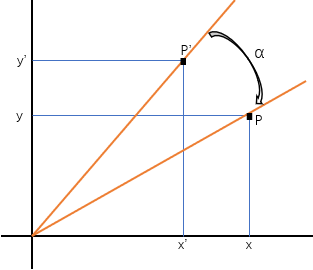
\includegraphics[scale=0.8]{./fig/3-1.png}
    \caption{在二位空间的转动}
\end{figure}
同学们应注意,在此过程中图3-1的坐标轴不动,而点动。此问题也可描述为坐标轴沿相反方向转动,即转$-\alpha$角:
\[
R_{axis}=
\begin{pmatrix}
    \cos \alpha & \sin\alpha \\
    -\sin\alpha & \cos \alpha
\end{pmatrix}    
\tag{3-62}
\]
存在着这两种观点,而应记住的一重要点是点的转动变换与坐标系转动的作用相反。

将二维转动变换的矩阵表示记住,现在观察三维转动。有许多考虑三维转动的方式,但所有这些方式都具有两个共同的原则。
第一,一般讲,需要用三个角来描述转动。读者对不对称物体做一演习就会相信这一点了。
第二,描述转动的习惯方式是按下列顺序:

(a)绕一坐标轴转$\phi$角。

(b)绕新位置的另一坐标轴转$\theta$角。

(c)再绕新位置的原坐标轴转$\psi$角。

这种转动顺序称为欧拉角转动(以数学家欧拉命名的)现代的作者们选择各种不同的顺序,因而同学们应小心地注意每一作者的习惯。为了和许多著名的教科书一致,我们的选择如图3-2所示。
\begin{figure}[htbp]
    \centering
    \begin{minipage}[t]{0.3\textwidth}
    \centering
    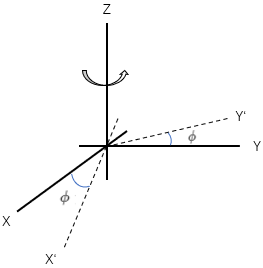
\includegraphics[width=4.5cm]{./fig/3-2a.png}
    (a)
    \end{minipage}
    \begin{minipage}[t]{0.3\textwidth}
    \centering
    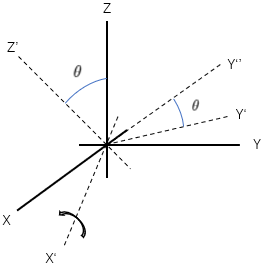
\includegraphics[width=4.5cm]{./fig/3-2b.png}
    (b)
    \end{minipage}
    \begin{minipage}[t]{0.3\textwidth}
    \centering
    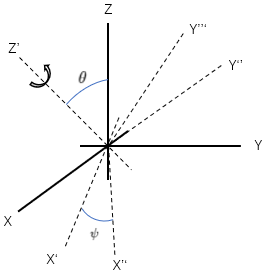
\includegraphics[width=4.5cm]{./fig/3-2c.png}
    (c)
    \end{minipage}
    \caption{在三维中转欧拉角(a)绕Z轴旋转$\phi(A)$; (b)绕X'轴旋转$\theta(B)$; (c)绕Z'轴旋转$\psi(C)$}
\end{figure}

(a)绕Z轴转$\phi$角得新的X'Y'Z坐标系(矩阵表示A)。

(b)绕X'轴转$\theta$角得新的X'Y''Z'坐标系\footnote{图B原书上Z'少了'。}(矩阵表示B)。

(c)绕Z'轴转$\psi$角得新的最终的X''Y'''Z'坐标系(矩阵表示C)。

此动作顺序表示坐标系转动。每一分步变换的矩阵表示可用与方程3-62类比的方法求出,它们是
\[A=
\begin{pmatrix}
    \cos \phi & \sin\phi & 0 \\
    -\sin\phi & \cos \phi & 0 \\
    0 & 0 & 1
\end{pmatrix}
\tag{3-63a}
\]
\[B=
\begin{pmatrix}
    1 & 0 & 0 \\
    0 & \cos \theta & \sin\theta \\
    0 & -\sin\theta & \cos \theta
\end{pmatrix}
\tag{3-63b}
\]
\[C=
\begin{pmatrix}
    \cos \psi & \sin\psi & 0 \\
    -\sin\psi & \cos \psi & 0 \\
    0 & 0 & 1
\end{pmatrix}
\tag{3-63c}
\]
三个分步转动的总效应给出一般化的三维转动矩阵$R=ABC$\footnote{因下式长度问题,这里稍微对原式做些许改动。},
\[R=
\begin{pmatrix}
    \cos \psi \cos \phi-\cos \theta \sin\phi \sin\psi & \cos \psi \sin\phi+\cos \theta \cos \phi \sin\psi & \sin\psi \sin\theta \\
    -\sin\psi \cos \phi-\cos \theta \sin\phi \cos \psi & -\sin\psi \sin\phi+\cos \theta \cos \phi \cos \psi & \cos \psi \sin\theta \\
    \sin\theta \sin\phi & -\sin\theta \cos \phi & \cos \theta
\end{pmatrix}
\tag{3-64}
\]
它虽然很复杂,但在讨论分子转动中很重要。

做为本节的总结和前两节的部分提纲,下表列出有关变换、矩阵、行列式和线性无关的表述之间的相互关系。同学们应努力掌握此课题的内在联系并应用它。
\begin{center}
    \textbf{等价表述; $n \times n$矩阵}\\
    \textbf{情况1. 行列式不为零}
\end{center}

1.向量组线性无关。

2.单位矩阵的行等价。

3.矩阵有逆。

4.矩阵的秩$r$等于维数$n$。

5.线性变换是$n$空间到$n$空间一对一的映射。

6.矩阵的行列式不为零。

7.含$n$个未知数的$n$个联立方程有解。

\begin{center}
    \textbf{情况2.行列式为零}
\end{center}

1.向量组线性相关。

2.是至少有一全为零的行的三角矩阵的行等价矩阵。

3.矩阵无逆。

4.矩阵的秩$r$小于维数$n$。

5.线性变换是$n$空间到$n$空间的$r$-维子空间的多对一的映射。

6.矩阵的行列式为零。

7.含$n$个未知数的$n$个齐次联立线性方程有解。

\begin{center}
    \textbf{等价表述:秩为$r$的$m \times n$矩阵}
\end{center}

1. $m$个向量中任何$r$个向量线性无关,$m-r$个向量是$r$个独立向量的因向量。

2.是有$m-r$个全为零的行的三角矩阵的行等价矩阵。

3.线性变换是$n$空间到$m$空间的$r$-维子空间的映射。

4.若增广矩阵的秩也是$r$,则联立线性方程组有解。

\section{线性算符}

本节在应用向量空间代数于量子力学方面将迈进主要的一步。早在第一章我们就讲过量子力学的本征值方程的作用,并见过这样方程所取的形式,如方程1-2。
虽然对特殊算符的描述要留给量子力学著作来讨论,但在这里能列出其一般结果。按我们的习惯先介绍一些定义。

\begin{definition}[算符]
    算符是定义在某向量空间变该空间中一向量为另一向量的一组指令。
    由此,我们写下$\mathscr{A}\xi=\eta$来表示,将体现在算符$\mathscr{A}$的定义中的一组特定指令作用于向量$\xi$形成一新向量$\eta$。用草体字表示算符。
\end{definition}

我们要问算符的这个定义和变换的定义之间有何区别。经最终分析可以说它们没有区别。
算符一词在量子力学的行文中常用于表示特定物理量,而变换一词则用于表示坐标系的改变。
无论如何,它们的定义在形式上是相同的,而且线性算符的定义和线性变换的定义也是相似的。

\begin{definition}[线性算符]
    线性算符服从下列方程:\\
    (a) $\mathscr{A}(c\xi)=c\mathscr{A}\xi$,式中$c$是常数(也可能是复数)。\\
    (b) $\mathscr{A}(\xi+\eta)=\mathscr{A}\xi+\mathscr{A}\eta$,式中$\xi$和$\eta$都是向量。
\end{definition}

算符表示“一组指令”这一定义并未给出表示算符的方式。那么怎样表示线性算符呢?
算符$\mathscr{A}$作用于任一向量的结果可从算符$\mathscr{A}$作用于基向量的结果求出。
例如,设已知
\[\mathscr{A}\phi^i=\sum_jA_{ij}\phi^j \tag{3-65}\]
式中向量组$\{\phi^i\}$,$\{\phi^j\}$是所讨论的向量空间中两组完备正交归一基向量组。
任一向量都可在$\{\phi^i\}$,$\{\phi^j\}$下展开\footnote{原文为“任一向量都可展开成$\phi^j$”,感觉翻译有问题。}:
\[\xi=\sum_ic_i\phi^i \qquad \eta=\sum_id_j\phi^j \tag{3-66}\]
我们再用算符定义$\mathscr{A}\xi=\eta$,将数$\{c_i\}$和$\{d_i\}$联系起来:
\[\mathscr{A}\xi=\mathscr{A}\sum_ic_i\phi^i=\sum_{ij}c_iA_{ij}\phi^j=\eta=\sum_jd_j\phi^j \tag{3-67}\]
因此,
\[d_j=\sum_iA_{ij}c_i \tag{3-68}\]
现在只需揭示出数$\{A_{ij}\}$是什么。若基向量$\{\phi^i\}$是正交归一的,那就容易办到,
\[\bra*{\phi^j}\ket*{\mathscr{A}\phi^i}=\sum_k\bra*{\phi^j}\ket*{A_{ik}\phi^k}=\sum_kA_{ik}\bra*{\phi^j}\ket*{\phi^k}=A_{ij} \tag{3-69}\]
我们时常见到方程3-69左边的那条竖线$\bra*{\phi^j}\mathscr{A}\ket*{\phi^i}$,此特殊竖线并未增加新的含义,只是提醒注意中心的算符$\mathscr{A}$。
像$\bra*{\phi^j}\mathscr{A}\ket*{\phi^i}$这样的内积常称为矩阵元。接下去我们就会看到使用这些矩阵元带来很大的方便。
例如,方程3-68现在可写成
\[d_j=\sum_i\bra*{\phi^j}\mathscr{A}\ket*{\phi^i}c_i \tag{3-70}\]
它具有矩阵乘积的形式\footnote{原书这里写得很乱,这里稍微修整了一下。},
\[
\begin{pmatrix}
    d_1 \\ d_2 \\ \vdots \\ d_n
\end{pmatrix}    
=
\begin{pmatrix}
    \bra*{\phi^1}\mathscr{A}\ket*{\phi^1} & \bra*{\phi^1}\mathscr{A}\ket*{\phi^2} & \cdots & \bra*{\phi^1}\mathscr{A}\ket*{\phi^n} \\
    \bra*{\phi^2}\mathscr{A}\ket*{\phi^1} & \bra*{\phi^2}\mathscr{A}\ket*{\phi^2} & \cdots & \bra*{\phi^2}\mathscr{A}\ket*{\phi^n} \\
    \vdots & \vdots & \ddots & \vdots \\
    \bra*{\phi^n}\mathscr{A}\ket*{\phi^1} & \bra*{\phi^n}\mathscr{A}\ket*{\phi^2} & \cdots & \bra*{\phi^n}\mathscr{A}\ket*{\phi^n}
\end{pmatrix}
\begin{pmatrix}
    c_1 \\ c_2 \\ \vdots \\ c_n
\end{pmatrix} 
\tag{3-71}
\]
在此情况下我们除去了展开系数$A_{ij}$(小体大写字母),并代之以通常的矩阵元$a_{ji}=\bra*{\phi^j}\mathscr{A}\ket*{\phi^i}$:
\[d_j=\sum_iA_{ij}c_i=\sum_ia_{ji}c_i \tag{3-72}\]
在这里我们用列矩阵($n \times 1$矩阵)表示向量。若左向量写成$1 \times n$行矩阵在向量写成$n \times 1$列矩阵,则内积可由用矩阵符号表示的二向量形成。它们的乘积自然是$1 \times 1$矩阵或标量:
\[\bra*{\xi}\ket*{\eta}=\left(c_1^* \ c_2^* \ \cdots \ c_n^*\right)
\begin{pmatrix}
    d_1 \\ d_2 \\ \vdots \\ d_n
\end{pmatrix}
=\sum_{i=1}^nc_i^*d_i \tag{3-73}\]
在我们讨论的情况,$\eta=\mathscr{A}\xi$。因此,
\[\bra*{\xi}\ket*{\eta}=\bra*{\xi}\mathscr{A}\ket*{\xi}=\left(c_1^* \ c_2^* \ \cdots \ c_n^*\right)
\begin{pmatrix}
    a_{11} & a_{12} & \cdots & a_{1n} \\
    a_{21} & a_{22} & \cdots & a_{2n} \\
    \vdots & \vdots & \ddots & \vdots \\
    a_{n1} & a_{n2} & \cdots & a_{nn}
\end{pmatrix}
\begin{pmatrix}
    d_1 \\ d_2 \\ \vdots \\ d_n
\end{pmatrix}
\tag{3-74}\]

现在出现了两个重要特点。用方阵表示线性算符和用列矩阵表示向量。
由于定义矩阵元为$a_{ji}=\bra*{\phi^j}\mathscr{A}\ket*{\phi^i}$,故所用的矩阵依赖于基组$\{\phi^i\}$的选择。
当然任何基组都可用。因此,有许多表示$\mathscr{A}$的矩阵,不同的矩阵表示产生于不同的基。
因此,严格讲,说算符$\mathscr{A}$与其矩阵元为$a_{ij}$的矩阵$A$相同是不正确的;
应该说,矩阵表示$\mathscr{A}$,或矩阵是算符$\mathscr{A}$的以$\{\phi^i\}$为基的表示。
同样地,说$\eta$与列向量
\[
\begin{pmatrix}
    d_1 \\ d_2 \\ \vdots \\ d_n
\end{pmatrix}
\]
相同也是不正确的,应该说,此列向量是$\eta$的表示或此列向量表示$\eta$。

我们还应考察一给定算符的二矩阵表示之间的关系。令$A^{\phi}$为$\mathscr{A}$的以$\{\phi^i\}$为基的表示,$A^{\psi}$为$\mathscr{A}$的以$\{\psi^i\}$为基的表示。
矩阵元为$a_{ij}^{\phi}=\bra*{\phi^i}\mathscr{A}\ket*{\phi^j}$和$a_{ij}^{\psi}=\bra*{\psi^i}\mathscr{A}\ket*{\psi^j}$。又设二基(正交归一的)以酉变换
\[\psi^i=\sum_ku_{ik}\phi^k\]
相关联,反过来,
\[\phi^i=\sum_ju^*_{ji}\psi^j=\sum_ju'^*_{ij}\psi^j\]
于是,矩阵元$a_{ij}^{\phi}$与$a_{ij}^{\psi}$之间的关系为
\[a_{ij}^{\psi}=\bra*{\psi^i}\mathscr{A}\ket*{\psi^j}=\sum_ku^*_{ik}\bra*{\phi^k}\mathscr{A}\ket*{\psi^j}=\sum_{kl}u^*_{ik}u_{jl}\bra*{\phi^k}\mathscr{A}\ket*{\phi^l}=\sum_{kl}u^*_{ik}u_{jl}a_{kl}^{\phi}\]
\[=\sum_{kl}u_{ik}'^{-1}a_{kl}^{\phi}u_{lj}'=[U'^{-1}A^{\phi}U']_{ij} \tag{3-75}\]
结构$A^{\psi}=U'^{-1}A^{\phi}U'$经常出现在代数方程组中。若$A=S^{-1}BS$,我们就说对B进行相似变换得到A。
若$S$是酉矩阵(现在$S=U'$),则变换称为酉变换。由此得出下列结果。

\begin{theorem}
    $\mathscr{A}$的以$\psi$为基的矩阵表示可通过对$\mathscr{A}$的以$\phi$为基的矩阵表示作相似变换得出;这个相似变换就是联系二基的变换的转置。
\end{theorem}

我们建立了线性算符和它们的矩阵表示之间的关系;它只是矩阵代数的概念,矩阵乘积,逆矩阵和转置矩阵对算符的自然推广。还有一些概念很重要,它们包含在下列定义中。

\begin{definition}[换位子,伴算子]
    二算符$\mathscr{A}$和$\mathscr{B}$的换位子是$\mathscr{A}\mathscr{B}-\mathscr{B}\mathscr{A}$,记着$[\mathscr{A},\mathscr{B}]$。
    算符$\mathscr{A}$的伴算符,记着$\mathscr{A}^{\dagger}$,其矩阵元和$\mathscr{A}$的矩阵元有如下关系:
    \[\bra*{\phi^i}\mathscr{A}^{\dagger}\ket*{\phi^j}=\bra*{\mathscr{A}\phi^i}\ket*{\phi^j}\]    
\end{definition}

$\mathscr{A}$的伴算符的矩阵是$\mathscr{A}$的矩阵表示转置并共轭化,因
\[\bra*{\phi^i}\ket*{\mathscr{A}^{\dagger}\phi^j}=\bra*{\mathscr{A}\phi^i}\ket*{\phi^j}=\bra*{\phi^j}\mathscr{A}\ket*{\phi^i}^* \tag{3-76}\]
剑号表示伴算符。

\begin{definition}[迹]
    算符的迹是算符的任何矩阵表示的对角元之和:
    \[\text{tr}\mathscr{A}=\sum_ia_{ii}\]
    (德语文献中迹称为Spur并简写为Sp)
\end{definition}

考虑一典型算符及其一些不同基的表示,做为已讨论的某些原则的例子。

\begin{definition}[投影算符]
    将某向量投影到一单位向量$\epsilon$的方向上的投影算符$\sigma_{\epsilon}$。定义为$\sigma_{\epsilon}\xi=\bra*{\epsilon}\ket*{\xi}\epsilon$。
\end{definition}

投影算符给出一向量在特定方向上的分量。应用算符法就能非常简便地解出$\sigma_{\epsilon}$的特征值:
\[\sigma_{\epsilon}^2\xi=\sigma_{\epsilon}(\sigma_{\epsilon}\xi)=\sigma_{\epsilon}(\bra*{\epsilon}\ket*{\xi}\epsilon)=\bra*{\epsilon}\ket*{\xi}\sigma_{\epsilon}\epsilon=\bra*{\epsilon}\ket*{\xi}\epsilon \tag{3-77}\]

因此,$\sigma_{\epsilon}^2=\sigma_{\epsilon}$。这表示算符$\sigma_{\epsilon}$是“幂等的”($idempotent$)由此可
得,$(\sigma_{\epsilon}^2-\sigma_{\epsilon})=0=\sigma_{\epsilon}(\sigma_{\epsilon}-1)=0$,即$\sigma_{\epsilon}=0$或$\sigma_{\epsilon}=1$。
即便不写出$\sigma_{\epsilon}$的矩阵表示,我们就已经知道$\sigma_{\epsilon}$的本征值(一或零)。
现在让我们看看$\sigma_{\epsilon}$的矩阵表示是什么样。

\textbf{例}

在二维欧氏向量空间投影方向向量为$\epsilon=(1/\sqrt{2},1/\sqrt{2})$的投影算符。
取习用的笛卡儿基$\phi^1=(1,0)$, $\phi^2=(0,1)$为基。用直接法得出
\[p_{11}^{\phi}=\bra*{\phi^1}\sigma\ket*{\phi^1}=\bra*{(1,0)}\ket*{\left(\frac{1}{\sqrt{2}},\frac{1}{\sqrt{2}}\right)\left(\frac{1}{\sqrt{2}}\right)}=\frac{1}{\sqrt{2}} \cdot \frac{1}{\sqrt{2}}=\frac{1}{2}\]
\[p_{12}^{\phi}=\frac{1}{2} \qquad p_{21}^{\phi}=\frac{1}{2} \qquad p_{22}^{\phi}=\frac{1}{2}\]
矩阵$P^{\phi}$为
\[
\begin{pmatrix}
    \frac{1}{2} & \frac{1}{2} \\ \frac{1}{2} & \frac{1}{2}
\end{pmatrix}    
\]
再考虑基$\psi^1=(1/2,\sqrt{3}/2)$, $\psi^2=(\sqrt{3}/2,-1/2)$的情况。用同样的计算方法,得出矩阵元$p_{ij}^{\psi}$和矩阵
\[P^{\psi}=
\begin{pmatrix}
    \frac{1}{2}+\frac{\sqrt{3}}{4} & \frac{1}{4} \\
    \frac{1}{4} & \frac{1}{2}-\frac{\sqrt{3}}{4}
\end{pmatrix}
\]
现在应验证一下变换定理,$P^{\psi}=U'^{-1}P^{\phi}U'$。因\footnote{原书下式第一个$\phi^2$的系数误写成了$\frac{\sqrt{2}}{2}$(笑)。}
\[\psi^1=\frac{1}{2}(1,0)+\frac{\sqrt{3}}{2}(0,1)=\frac{1}{2}\phi^1+\frac{\sqrt{3}}{2}\phi^2\]
\[\psi^2=\frac{\sqrt{3}}{2}(1,0)-\frac{1}{2}(0,1)=\frac{\sqrt{3}}{2}\phi^1-\frac{1}{2}\phi^2\]
所以
\[
U=
\begin{pmatrix}
    \frac{1}{2} & \frac{\sqrt{3}}{2} \\
    \frac{\sqrt{3}}{2} & -\frac{1}{2}
\end{pmatrix}
\qquad
U'=
\begin{pmatrix}
    \frac{1}{2} & \frac{\sqrt{3}}{2} \\
    \frac{\sqrt{3}}{2} & -\frac{1}{2}
\end{pmatrix}
U'^{-1}=
\begin{pmatrix}
    \frac{1}{2} & \frac{\sqrt{3}}{2} \\
    \frac{\sqrt{3}}{2} & -\frac{1}{2}
\end{pmatrix}
\]
直接相乘
\[
\begin{pmatrix}
    \frac{1}{2} & \frac{\sqrt{3}}{2} \\
    \frac{\sqrt{3}}{2} & -\frac{1}{2}
\end{pmatrix}   
\begin{pmatrix}
    \frac{1}{2} & \frac{1}{2} \\
    \frac{1}{2} & \frac{1}{2}
\end{pmatrix}
\begin{pmatrix}
    \frac{1}{2} & \frac{\sqrt{3}}{2} \\
    \frac{\sqrt{3}}{2} & -\frac{1}{2}
\end{pmatrix}
=
\begin{pmatrix}
    \frac{1}{2}+\frac{\sqrt{3}}{4} & \frac{1}{4} \\
    \frac{1}{4} & \frac{1}{2}-\frac{\sqrt{3}}{4}
\end{pmatrix}
=P^{\psi}
\]
我们可很快地求出,以$x^1=(1/\sqrt{2},1/\sqrt{2})$, $x^2=(1/\sqrt{2},1/\sqrt{2})$为基时$P$的形式为
\[
\begin{pmatrix}
    1 & 0 \\ 0 & 0
\end{pmatrix}    
\]
我们可以用这三个例子并结合图3-3(有点滑稽\footnote{确实(笑死)。})说明矩阵表示的概念。
\begin{figure}[htbp]
    \centering
    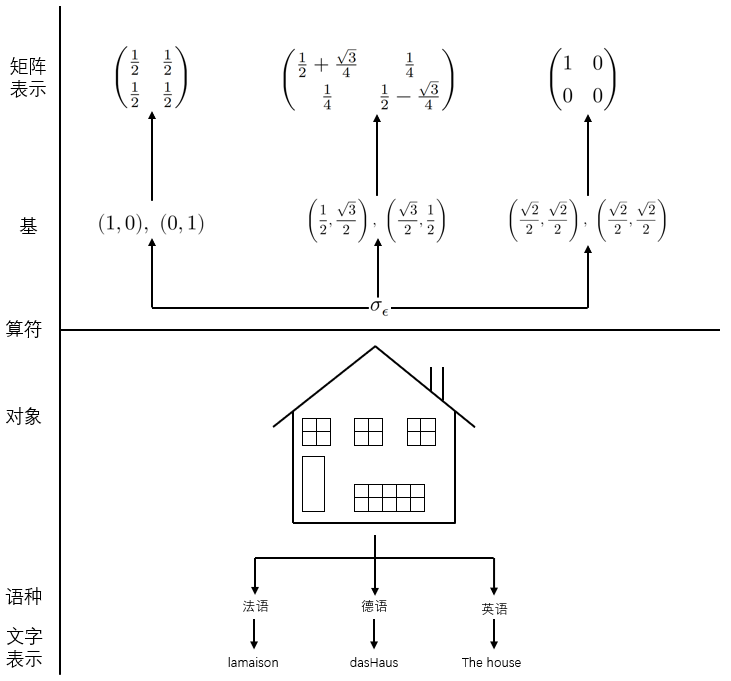
\includegraphics[scale=0.7]{./fig/3-3.png}
    \caption{算符$\sigma_{\epsilon}$, $\epsilon=(1/\sqrt{2},1/\sqrt{2})$及其在三个基上的矩阵表示;类比,对象房子,和在三个语种中的文字表示}
\end{figure}
最后我们讲,求线性算符的特征值和特征向量问题。井非所有线性算符都服从特征值方程,但从量子力学的观点看,有两类非常重要的算符服从特征值方程。
这些算符是厄米算符和酉算符,我们先概述一下结果,然后再证明。

\begin{definition}[简并特征值,简并度]
    若一特征值满足在同一个特征向量方程中对应多个特征向量\footnote{原文为“若一特征值满足多于一个特征向量的特征值一特征向量方程”,不知道翻译了个什么东西。},则称该特征值为简并的;特征值相同的特征向量数称为特征值的简并度。
\end{definition}

\begin{definition}[厄米算符]
    厄米算符是自伴的线性算符; 即$\mathscr{H}=\mathscr{H}^{\dagger}$或$h_{ij}=h_{ji}^*$。厄米矩阵的对角元是实的。
\end{definition}

\begin{theorem}
    在n维向量空间里的厄米算符有$n$个不同的特征向量和$n$个实特征值。
    若特征值是非简并的,则特征向量彼此正交,再乘以适合的归一化常数就形成正交归一向量组。
    即使某些特征向量是简并的,也可由不同的特征向量造正交归一组。
\end{theorem}

\begin{definition}[酉算符]
    酉算符是线性算符,其伴等于其逆:$\mathscr{U}^{-1}=\mathscr{U}^{\dagger}$。
\end{definition}

\begin{theorem}
    在n维向量空间的酉算符有$n$个不同的特征向量(如上,可形成正交归一组)和$n$个特征值,它们全都具有单位模。
\end{theorem}

我们从证明厄来定理开始。若$\mathscr{H}\phi^i=h_i\phi^i$,则$\bra*{\phi^i}\mathscr{H}\ket*{\phi^i}=h_i\bra*{\phi^i}\ket*{\phi^i}$。
因$\mathscr{H}$是厄米的,所以$\bra*{\phi^i}\mathscr{H}\ket*{\phi^i}=\bra*{\phi^i}\mathscr{H}\ket*{\phi^i}^*$, $h_i=h_i^*$,因而$h_i$是实的。
对于二不同的特征向量,
\[\mathscr{H}\phi^i=h_i\phi^i \tag{3-78a}\]
\[\mathscr{H}\phi^j=h_j\phi^j \tag{3-78a}\]
从方程3-78a得出$\bra*{\phi^i}\mathscr{H}\ket*{\phi^i}=h_i\bra*{\phi^i}\ket*{\phi^i}$;
从方程3-78b得出$\bra*{\mathscr{H}\phi^j}\ket*{\phi^i}=h_j^*\bra*{\phi^j}\ket*{\phi^i}$。
然而,$\bra*{\mathscr{H}\phi^j}\ket*{\phi^i}=\bra*{\phi^i}\mathscr{H}\ket*{\phi^j}^*=\bra*{\phi^j}\ket*{\mathscr{H}\phi^i}=h_i\bra*{\phi^j}\ket*{\phi^i}$
因此$(h_i-h_j^*)\bra*{\phi^j}\ket*{\phi^i}=0$,因$h_j$为实的,
当$h_i \neq h_j$时,则$\bra*{\phi^j}\ket*{\phi^i}=0$,因而特征向量是正交的。

对酉算符定理的证明很相似。若$\mathscr{U}\psi^i=u_i\psi^i$,则$\mathscr{U}^{\dagger}\mathscr{U}\psi^i=\mathscr{U}^{\dagger}u_i\psi^i=u_i\mathscr{U}^{\dagger}\psi^i$。
因此$\mathscr{U}^{\dagger}\psi^i=\left(\frac{1}{u_i}\right)\psi^i$或$\mathscr{U}^{\dagger}$的特征向量和$\mathscr{U}$的特征向量相同,而其特征值是$\mathscr{U}$的特征值的倒数。
于是,$\bra*{\psi^i}\mathscr{U}^{\dagger}\ket*{\psi^i}=u_i\bra*{\psi^i}\ket*{\psi^i}$, $\bra*{\mathscr{U}^{\dagger}\psi^i}\ket*{\psi^i}=(1/u_i^*)\bra*{\psi^i}\ket*{\psi^i}$。
但$\bra*{\mathscr{U}^{\dagger}\psi^i}\ket*{\psi^i}$又等于$\bra*{\psi^i}\mathscr{U}^{\dagger}\ket*{\psi^i}$,因此$1/u_i^*=u_i$, $u_i^*u_i=1$,或特征值$u_i$的模为一。
可用证明厄来算符类似的方法证明特征向量的正交性。由简并特征值产生的特殊问题在本节末讨论。

这些证明都未说明厄米算符或酉算符为什么必须服从特征值方程,现在只给结果而不加证明。无论如何,这些定理中的每一个都有在欧氏向量空间中的推论。
\begin{proposition}
    对应于厄米向量空间中的厄米算符定理,在欧氏向量空间中有一对称算符$(\delta_{ij}=\delta_{ji})$的类似定理;
    对应于厄米向量空间中的酉算符定理,在欧氏向量空间中有一正交算符$(\mathfrak{R}'=\mathfrak{R}^{-1})$的类似的定理。
\end{proposition}

所有定理和推论涉及的都是特征值和特征向量的存在问题,但到目前为止还未讲如何求这些本征值。
我们能够从两个观点(久期方程和相似变换)来研究解特征值方程的一般形式。

考虑一矩阵形式的特征值方程,方程1-2,
\[\mathfrak{Q}\phi=q\phi \tag{3-79}\]
此方程是许多用向量$\phi$的分量表示的线性方程的简要陈述:
\[
\begin{array}{c}
    \mathfrak{Q}_{11}\phi_1+\mathfrak{Q}_{12}\phi_2+ \cdots +\mathfrak{Q}_{1n}\phi_n=q\phi_1 \\
    \vdots \qquad \qquad \vdots \qquad \qquad \qquad \vdots \quad \qquad \vdots \\
    \mathfrak{Q}_{n1}\phi_1+\mathfrak{Q}_{n2}\phi_2+ \cdots +\mathfrak{Q}_{nn}\phi_n=q\phi_n \\
\end{array}    
\tag{3-80}
\]
将这些方程重新整理一下,可得一组含$n$个未知数$\phi_i$($\phi$的分量)的齐次联立方程:
\[
\begin{array}{c}
    (\mathfrak{Q}_{11}-q)\phi_1+\mathfrak{Q}_{12}\phi_2+ \cdots +\mathfrak{Q}_{1n}\phi_n=0 \\
    \mathfrak{Q}_{11}\phi_1+(\mathfrak{Q}_{12}-q)\phi_2+ \cdots +\mathfrak{Q}_{1n}\phi_n=0 \\
    \vdots \\
    \mathfrak{Q}_{n1}\phi_1+\mathfrak{Q}_{n2}\phi_2+ \cdots +(\mathfrak{Q}_{nn}-q)\phi_n=0 \\
\end{array}  
\tag{3-81}  
\]
我们已经学过,仅当系数行列式等于零时,这样的方程才有非全零解。由此得到的$q$的$n$次方程,称为久期方程:
\[
\begin{vmatrix}
    (\mathfrak{Q}_{11}-q) & \mathfrak{Q}_{12} & \cdots & \mathfrak{Q}_{1n} \\
    \mathfrak{Q}_{11} & (\mathfrak{Q}_{12}-q) & \cdots & \mathfrak{Q}_{1n} \\
    \vdots  & \vdots & \ddots  & \vdots \\
    \mathfrak{Q}_{n1} & \mathfrak{Q}_{n2} & \cdots & (\mathfrak{Q}_{nn}-q) \\
\end{vmatrix}    
=0 \tag{3-82}
\]
久期方程是量子力学中常见的方程。思考一下方程3-82的意义。若将方程3-82展开,可得到未知数$q$的$n$次多项式。
将解该方程的实际问题暂时放置一边,先注意出现的一个有意义的概念:方程有$n$个根。
前边证明了的定理说应有$n$个特征向量和$n$个特征值,现在看到了为什么。这是因为特征值是$n$次方程的解。
正如我们见过那样某些根当然可能相等,但我们不准备讨论此问题。

现在有$n$个特征值。对每个特征值可用方程组3-81解出特征向量的分量$\phi_i$。
因此,方程3-81最终给出$n$个特征向量,对每一特征值有一特征向量。
为了完成计算,还需将特征向量归一化。

概括讲,解矩阵特征值方程可用下列步骤:

1.写出并解久期方程;得出特征值。

2.将特征值(现在已知)代入特征值方程解出特征向量。

3.将特征向量归一化。

我们也可用第二个观点讨论特征值问题。假定我们已知矩阵的特征值和特征向量:
\[
\begin{array}{c}
    \mathfrak{Q}\phi^1=q_1\phi^1 \\
    \mathfrak{Q}\phi^2=q_2\phi^2 \\
    \vdots \quad \qquad \vdots \\
    \mathfrak{Q}\phi^n=q_n\phi^n 
\end{array}    
\tag{3-83}
\]
可将列向量一列挨一列排起来形成$n \times n$矩阵,如
\[
\Phi=
\begin{pmatrix}
    \phi^1_1 & \phi^2_1 & \cdots & \phi^n_1 \\
    \phi^1_2 & \phi^2_2 & \cdots & \phi^n_2 \\
    \vdots & \vdots & \ddots & \vdots \\
    \phi^1_n & \phi^2_n & \cdots & \phi^n_n 
\end{pmatrix}    
\tag{3-84}
\]
本征向量$\phi^i$形成矩阵$\Phi$的列。$\mathfrak{Q}$对$\Phi$作用产生其列为$q_i\phi^i$的矩阵:
\[
\mathfrak{Q}\Phi=
\begin{pmatrix}
    q_1\phi^1_1 & q_2\phi^2_1 & \cdots & q_n\phi^n_1 \\
    q_1\phi^1_2 & q_2\phi^2_2 & \cdots & q_n\phi^n_2 \\
    \vdots & \vdots & \ddots & \vdots \\
    q_1\phi^1_n & q_2\phi^2_n & \cdots & q_n\phi^n_n 
\end{pmatrix}  
=
\begin{pmatrix}
    \phi^1_1 & \phi^2_1 & \cdots & \phi^n_1 \\
    \phi^1_2 & \phi^2_2 & \cdots & \phi^n_2 \\
    \vdots & \vdots & \ddots & \vdots \\
    \phi^1_n & \phi^2_n & \cdots & \phi^n_n 
\end{pmatrix}
\begin{pmatrix}
    q_1 & 0 & \cdots & 0 \\
    0 & q_2 & \cdots & 0 \\
    \vdots & \vdots & \ddots & \vdots \\
    0 & 0 & \cdots & q_n
\end{pmatrix}
=\Phi \hat{q}
\tag{3-85}
\]
式中符号$\hat{q}$表示其对角元为$n$个特征值,其它矩阵元皆为零的矩阵。方程3-85两边皆乘以$\Phi^{-1}$给出,
\[\Phi^{-1}\mathfrak{Q}\Phi=\hat{q} \tag{3-86}\]
此式可表述如下:用由特征向量为列形成的矩阵对$\mathfrak{Q}$作相似变换,给出由$\mathfrak{Q}$的特征值形成的对角矩阵。

因此,若能找到将$\mathfrak{Q}$变换成对角矩阵方法(这叫做将矩阵$\mathfrak{Q}$对角化),则该相似变换的列是特征向量,对角矩阵的对角元是特征值。
这种步骤易为数学计算用,因而经常形成用计算机解特征值问题的基础。正如前边已证明那样,因向量$\phi^i$是正交归一的,故变换$\Phi^{-1}\mathfrak{Q}\Phi$是酉变换。
我们用求上边讨论过的$\sigma_{\epsilon}$。矩阵的特征值做为这些概念的例子。

\textbf{例}

考虑算符$\sigma_{\epsilon}$,其中$\epsilon=(1/\sqrt{2},1/\sqrt{2})$是取常用的笛卡儿基。投影算符在此基上的矩阵表示为前边求出那样是
\[
\begin{pmatrix}
    \frac{1}{2} & \frac{1}{2} \\ \frac{1}{2} & \frac{1}{2}
\end{pmatrix}    
\]
为了求此算符的特征值,我们解久期方程。
\[
\begin{vmatrix}
    \frac{1}{2}-p & \frac{1}{2} \\ \frac{1}{2} & \frac{1}{2}-p
\end{vmatrix}    
=0
\]
展开给出二次多项式。
\[\frac{1}{4}-p+p^2-\frac{1}{4}=0\]
它的根是
\[p^2-p=0\]
\[p_1=1, \ p_2=0\]
这些根是$\sigma_{\epsilon}$的特征值,这正是前边单独根据算符性质所预言的那样。我们现在求对应于特征值$p_1=1$的特征向量$\phi^1$:
\[
\begin{pmatrix}
    \frac{1}{2} & \frac{1}{2} \\ \frac{1}{2} & \frac{1}{2}
\end{pmatrix} 
\begin{pmatrix}
    \phi_1^1 \\ \phi_2^1
\end{pmatrix} 
= 
\begin{pmatrix}
    \phi_1^1 \\ \phi_2^1
\end{pmatrix}  
\]
可写为
\[\frac{1}{2}\phi_1^1+\frac{1}{2}\phi_2^1=\phi_1^1 \qquad \frac{1}{2}\phi_1^1+\frac{1}{2}\phi_2^1=\phi_2^1\]
或
\[\phi_2^1=\phi_1^1 \qquad \phi_1^1=\phi_2^1\]
我们看到二特征向量——分量方程等同。为了完全确定这些分量,需要归一化,它给出$\phi_1^1=\phi_2^1=1/\sqrt{2}$,或$\phi^1=(1/\sqrt{2},1/\sqrt{2})$。
用同样方法可求出对应于$p_2=0$的特征向量$\phi^2=(1/\sqrt{2},-1/\sqrt{2})$。

停一下并对这些特征向量思考一番:特征值为一的特征向量和投影方向$\epsilon$完全一样;即在投影方向上的向量投影出长度相同的向量。
另一方面,特征值为零的特征向量$\phi^2$垂直于投影方向$\epsilon$;垂直于投影方向的向量投影到一点(零长度)。

我们也可以用直接代入法验证使$P$对角化的相似变换$\Phi^{-1}P\Phi$:
\[
\begin{pmatrix}
    \frac{1}{\sqrt{2}} & \frac{1}{\sqrt{2}} \\ \frac{1}{\sqrt{2}} & \frac{1}{\sqrt{2}}
\end{pmatrix} 
\begin{pmatrix}
    \frac{1}{2} & \frac{1}{2} \\ \frac{1}{2} & \frac{1}{2}
\end{pmatrix} 
\begin{pmatrix}
    \frac{1}{\sqrt{2}} & \frac{1}{\sqrt{2}} \\ \frac{1}{\sqrt{2}} & \frac{1}{\sqrt{2}}
\end{pmatrix} 
=
\begin{pmatrix}
    1 & 0 \\ 0 & 0
\end{pmatrix} 
\]
还有另外一种求特征向量的更简单些的技巧。向量的分量满足方程3-81。方程3-81中每一行像是行列式的余因式展开。
因为若$\phi_1=[\mathfrak{Q}-\hat{q}]_{11}$, $\phi_2=[\mathfrak{Q}-\hat{q}]_{12}$等等,则方程3-81的第一行给出
\[(\mathfrak{Q}_{11}-q)\phi_1+\mathfrak{Q}_{12}\phi_2+ \cdots +\mathfrak{Q}_{1n}\phi_n\]
\[=(\mathfrak{Q}_{11}-q)[\mathfrak{Q}-\hat{q}]_{11}+\mathfrak{Q}_{12}[\mathfrak{Q}-\hat{q}]_{12}+ \cdots +\mathfrak{Q}_{1n}[\mathfrak{Q}-\hat{q}]_{1n}=|\mathfrak{Q}-\hat{q}|=0 \tag{3-87}\]
式中数$\mathfrak{Q}_{ij}$,是$\mathfrak{Q}$的矩阵元,数$q$是$\mathfrak{Q}$的特征值。因此,久期行列式的任意行(第$i$行)的余因式给出与$\phi_i$成比例的数。

\textbf{例}

对于上述算符$\sigma_{\epsilon}$,特征值$p_1=1$的久期行列式为
\[
\begin{vmatrix}
    -\frac{1}{2} & \frac{1}{2} \\ \frac{1}{2} & -\frac{1}{2}
\end{vmatrix} 
=0   
\]
若取第一行的余因式,则特征向量$\phi^1$的分量与$(-1/2,-1/2)$成比例,若取第二行的余因式,则$\phi^1$的分量与$(-1/2,-1/2)$成比例,通过适当地归一化,征一种情况都给出$\phi^1=(1/\sqrt{2},1/\sqrt{2})$。

同学们可能要问,在什么条件下二算符有相同的特征向量组。这个问题在量子力学中很重要,因为它能告诉我们在什么情况下,二算符能同时取单一的稳定量态中确定的特征值。
这个问题的另一说法是在什么条件下,二矩阵能被同一相似变换对角化。结果是绝妙的简单。
\begin{theorem}
    当且仅当二厄米算符可对易时,此二算符能有相同的一组特征向量(特征函数)。
\end{theorem}

我们先证明,若$\mathscr{A}$和$\mathscr{B}$可对易,则它们有相同的特征向量。
设$\mathscr{A}$的特征向量是$\psi^i$,则$\mathscr{A}\psi^i=a_i\psi^i$。而因$\mathscr{A}$和$\mathscr{B}$可对易,
故$\mathscr{A}\mathscr{B}\psi^i=\mathscr{B}\mathscr{A}\psi^i$。于是\footnote{下式最后一个等号后可能少了个$\mathscr{B}$。}
\[\mathscr{B}\mathscr{A}\psi^i=\mathscr{A}\mathscr{B}\psi^i=\mathscr{B}a_i\psi^i=a_i(\mathscr{B}\psi^i) \tag{3-88}\]
方程3-88表明向量$(\mathscr{B}\psi^i)$也是$\mathscr{A}$的特征值为$a_i$,的特征向量。
它能成立的唯一条件是$(\mathscr{B}\psi^i)$为$\psi^i$的倍数;因此
\[\mathscr{B}\psi^i=b_i\psi^i \tag{3-89}\]
因而$\psi^i$也是$\mathscr{B}$的特征向量。同学们可以察觉出,若特征值是简并的,则上述论证不成立;在本节末再考虑这种情况。

为了证明逆定理——若$\mathscr{A}$和$\mathscr{B}$有相同的特征向量组,则它们可对易——我们先讲,如何用投影算符陈述一算符的效应。
向量$\xi$可在完备正交归一向量组$\{\phi^i\}$下展开\footnote{原文为“向量$\xi$可展成完备正交归一组$\phi^i$”,这翻译笑嘻了;并且3-90式最后一个等号后的$\sigma$原文还多了个上标$^i$。}:
\[\xi=\sum_i\bra*{\phi^i}\ket*{\xi}\phi^i=\sum_i\sigma_{\phi^i}\xi \tag{3-90}\]
即向量在一基上展开的效应与加和向量沿基向量的投影等价。
设$\mathscr{A}$的特征向量\footnote{说成特征向量集会更好。}是$\{\phi^i\}$。根据上述关系式可写出
\[\mathscr{A}\xi=\mathscr{A}\sum_i\bra*{\phi^i}\ket*{\xi}\phi^i=\sum_i\bra*{\phi^i}\ket*{\xi}a_i\phi^i=\sum_ia_i\sigma_{\phi^i}\xi \tag{3-91}\]
该方程可表述如下;算符作用于给定向量的效应等于该给定向量
沿特征向量的投影乘特征值的求和。若将$\mathscr{A}$表为
\[\mathscr{A}=\sum_ia_i\sigma_{\phi^i} \tag{3-91}\]
将$\mathscr{B}$(有同一特征向量组$\{\phi^i\}$)表为
\[\mathscr{B}=\sum_jb_j\sigma_{\phi^j} \tag{3-92}\]
不难证明$\mathscr{A}$和$\mathscr{B}$必须是可对易的,因
\[\left[\sum_ia_i\sigma_{\phi^i},\sum_jb_j\sigma_{\phi^j}\right]=0\]
(同学们应写出满意的换位子)。

本节的最后一个课题,是讨论在特征值简并时,线性算符的特征值和特征向量的性质应如何修正。
首先考虑在特征值简并时,如何从厄米算符(或酉算符、或对称算符,或正交算符)的特征向量形成正交归一向量组。

假定二特征向量$\xi_1$和$\xi_2$具有相同的特征值$q$。这些向量不必正交。定理只规定特征值不同的那些特征向量是正交的。
若$\mathscr{A}\xi_1=q\xi_1$, $\mathscr{A}\xi_2=q\xi_2$,则$\xi_1$和$\xi_2$的任何线性组合也服从特征值方程$\mathscr{A}(\xi_2+c\xi_1)=q(\xi_2+c\xi_1)$,$c$是常数。
我们要求$\xi_2+c\xi_1$(它是特征向量)是归一化的并与$\xi_1$正交。于是我们就有二个正交归一的向量$\xi_1$和$\xi_2+c\xi_1$。
准确地讲,我们面临的问题就是施密特正交化。设$\xi_1$已经是归一化的,并且
\[\bra*{\xi_1}\ket*{\xi_2+c\xi_1}=0 \tag{3-94}\]
可得出\footnote{原书下式笔误分母写成了$\bra*{\xi_1}\ket*{\xi_2}$。}
\[c=\frac{-\bra*{\xi_1}\ket*{\xi_2}}{\bra*{\xi_1}\ket*{\xi_1}}=-\bra*{\xi_1}\ket*{\xi_2} \tag{3-95}\]
此方程与方程3-9类似:可按特征值的简件度的要求,将此步骤面复进行下去。

简并性也影响对可对易算符共有的特征向量的讨论。我们已经指出过,若$\mathscr{A}$和$\mathscr{B}$是厄米的和可对易的,并且$\mathscr{A}$有特征向量$\{\psi^i\}$和特征值$\{a_i\}$则
\[\mathscr{A}(\mathscr{B}\psi^i)=a_i(\mathscr{B}\psi^i) \tag{3-88}\]
若$a_i$是非简并的特征值,则$\mathscr{B}\psi^i$是$\psi^i$的倍数。
但若$a_i$是简并的,则一般讲$\mathscr{B}\psi^i$是属于特征值$a_i$的所有特征向量的线性组合。
假设用第二个指标$k$来标记,是从$1$到$n$($a_i$是$n$重简并)则
\[\mathscr{B}\psi^i=\sum_kb_{ik}\psi^{ik} \tag{3-96}\]
系数$b_{ik}$形成$\mathscr{B}$的矩阵表示(非对角的)的$n$-维子矩阵。可用另一种方式表述:若$A$是对角矩阵,则在$A$的非简并域$B$也是对角的。
若A是简并的并且B也不是对角矩阵,则可用对小的子矩阵对角化的办法求$\mathscr{B}$的特征值。

本节介绍了一些简要阐述量子力学的核心概念。概述这些概念作为总结。

1.一旦基组指定了,线性算符就可用矩阵来表示。算符$\mathscr{A}$ 
的矩阵表示的矩阵元是$a_{ij}=\bra*{\phi^i}\mathscr{A}\ket*{\phi^i}$, $\{\phi^i\}$是指定的基组。

2.$\mathscr{A}$作用于向量$\xi$的效应相当于用$\xi$的列矩阵表示乘$\mathscr{A}$的矩阵表示。

3.用相似变换改变基。

4.厄米算符有实的特征值和正交归一的特征向量。

5.酉算符有模为一的特征值和正交归一的特征向量。

6.解特征值方程的方法有:(a)写出并解久期方程,代入将特征值方程并归一化;(b)解久期方程,用久期行列式的余因式求特征向量并归一化;(c)求使矩阵对角化的相似变换。

7.当且仅当二厄来算符可对易时,二算符就有相同的特征向量组。

\begin{problemset}
\item 若下列向量组是线性无关的,则用它们形成正交归一向量组;若它们是线性相关的,则写出线性关系式。

(a) (1,1,2), (0,-1,0), (-1,0,1)。

(b) (1,2,-1,0), (0,3,4,1), (1,1,1,1), (2,0,-4,1)。

(c) (i,1,2), (2i+1,-1,3i), (4,5i,6-i)。

(d) (0,0,2,0,0), (1,1,1,1,1), (1,3,1,2,2), (0,0,1,2,2), (1,0,1,0,1)。
\item 一组彼此正交的向量是否线性无关?为什么是或为什么不是?
\item 证明在向量空间中$c\alpha=0$表示或$c=0$,或$\alpha=0$。
\item 用题1中的(a),(b),(c)的全部向量造乘法表,并计算它们的内积。
\item 证明矩阵乘法服从结合律。
\item 设
\[
A=
\begin{pmatrix}
    1 & 2 & -1 \\
    3 & 0 & 2 \\
    4 & 5 & 0
\end{pmatrix}
\qquad
B=
\begin{pmatrix}
    1 & 0 & 0 \\
    2 & 1 & 0 \\
    0 & 1 & 3
\end{pmatrix}
\]
求$AB$和$BA$。$A$和$B$是否可对易?求$A^{-1}$和$B^{-1}$。证明$(AB)'=B'A'$, $(AB)^{-1}=B^{-1}A^{-1}$。
\item 用余因式展开和直接法求算行列式
\[
\begin{vmatrix}
    1 & -1 & 1 & -1 \\
    0 & 1 & -1 & 1 \\
    0 & 0 & 1 & -1 \\
    0 & 0 & 0 & 1
\end{vmatrix}    
\]
\item 一行列式其主对角线下各元皆为零,主对角线和主对角线上各元不为零。证明行列式的值就是对角元的乘积。
\item 下列联立线性方程组,若有解则解之,若无解则说明原因。
\[
(a)
\left \{
\begin{array}{c}
    2x-3y+5z=0 \\ x-y-2z=2 \\ 5x-z=-1
\end{array}
\right .
\]
\[
(b)
\left \{
\begin{array}{c}
    2x-y+3z-w=0 \\ 4x-2y-z+3w=0 \\ 2x-y-4z+4w=0 \\ 10x-5y-6z+10w=0
\end{array}
\right .
\]
\[
(c)
\left \{
\begin{array}{c}
    2x-y+3z=1 \\ 4x-2y-z=-3 \\ 2x-y-4z=-4 \\ 10x-5y-6z=10
\end{array}
\right .
\]
\[
(d)
\left \{
\begin{array}{c}
    4x+2y+z=11 \\ x-y-z=-4 \\ x+y+z=6
\end{array}
\right .
\]
\item 什么样的正交变换可使笛卡儿基$(\hat{x},\hat{y},\hat{z})$变为球极基$(\hat{r},\hat{\theta},\hat{\phi})$?
\item 有一线性变换
\[
L=
\begin{pmatrix}
    2 & -1 \\ -3 & 0
\end{pmatrix}    
\]
可将$xy$面变成$UV$面。在$L$变换下求点(1,2), (-2,1), (1,0), (0,1)的像。
\item 计算下列每个变换的秩并做说明。
\[
(a)
\left \{
\begin{array}{c}
    u=x+2y-3z \\ v=2x-y+4z \\ w=3x+y+z
\end{array}
\right .
\]
\[
(b)
\left \{
\begin{array}{c}
    u=y-z \\ v=x-y+3z \\ w=x+z
\end{array}
\right .
\]
\item 在2-维厄来空间二基的关系为
\[\psi^1=\frac{1}{\sqrt{2}}(\phi^1+i\phi^2) \qquad \psi^2=\frac{1}{\sqrt{2}}(\phi^1-i\phi^2)\]

(a)确定将$\phi$向量变换为$\psi$向量的西矩阵。

(b)若在$\phi$表中算符$\mathscr{A}$的矩阵表示为
\[
A^{\phi}=
\begin{pmatrix}
    \cos \alpha & -\sin\alpha \\ \sin\alpha & \cos \alpha 
\end{pmatrix}
\]
求在$\psi$表示中其矩阵表示$A^{\psi}$?

(c)证明酉变换或正交变换总有逆。
\item 有一相似变换$B=T^{-1}AT$,其中$T$为
\[
T=
\begin{pmatrix}
    \cos \theta & -\sin\theta \\ \sin\theta & \cos \theta 
\end{pmatrix}    
\]
证明用此相似变换可将对称的实的矩阵
$
A=
\begin{pmatrix}
    a & b \\ b & b 
\end{pmatrix}    
$
变换为对角矩阵
$
B=
\begin{pmatrix}
    c & 0 \\ 0 & d 
\end{pmatrix}    
$
导出实现对角化变换的$\theta$值,并求算$c$和$d$。
\item 证明厄米算符的下列性质。

(a)厄米算符的任何矩阵表示都有实行列式。

(b)厄米算符的逆也是厄米的。

(c)当和仅当二厄来算符是可对易时,它们的乘积是厄米的。

16.求迹的下列性质。

(a) $trA^{-1}=(trA)^*$

(b) $tr(aA)=atrA$

(c) $tr(A+B)=trA+trB$

(d) $tr(AB)=tr(BA)$

(e) $tr(A)$与$\mathscr{A}$的表示$A$的基无关。
\item 证明酉算符总可写成下列形式。

(a)形式$\mathscr{U}=\mathscr{A}+i\mathscr{B}$,式中$\mathscr{A}$和$\mathscr{B}$是厄米的,$[\mathscr{A},\mathscr{B}]=0$。

(b)形式$\mathscr{U}=e^{i\mathscr{A}}$,式中$\mathscr{A}$是厄米的。
\item 证明正交算符和酉算符的下列性质。

(a)二正交算符的乘积是正交的。

(b)若$\mathscr{A}$是对称的,$\mathscr{U}$是正交的,则$\mathscr{U}^{-1}\mathscr{A}\mathscr{U}$是对称的。

(c)二酉算符的乘积也是酉算符。

(d)若$\mathscr{A}$是厄米算符,$\mathscr{U}$是酉算符,则$\mathscr{U}^{-1}\mathscr{A}\mathscr{U}$是厄米的。
\item 证明方程3-64是在3D空间表示欧拉角转动的矩阵。
\item 若特征值是简并的,则在确定特征向量时会遇到什么情况?
\item 求算符$\mathscr{K}$的特征值和特征向量,$\mathscr{K}$在3D空间的矩阵表示是
\[
K=
\begin{pmatrix}
    7 & -3 & -\sqrt{2} \\ -3 & 7 & \sqrt{2} \\ \sqrt{2} & \sqrt{2} & 10
\end{pmatrix}
\]
用适当的相似变换使$K$对角化以验证前边求出的结果。
\item 证明酉算符的特征向量是正交的。
\item 求$\begin{pmatrix}1 & i & 0 \\ -i & 1 & 0 \\ 0 & 0 & 0\end{pmatrix}$的特征值和特征向量。
\end{problemset}
\chapter{经典力学}
本章的目的有两个。\footnote{原文为“本章的目的是双重的。”,机翻味太浓了(乐}首先将经典力学表示成,使经典力学和量子力学之间的联系显明的那样形式。

第二个目的是学习掌握量子化学中重要的二力学问题,即分子的振动和转动。这两种分子运动是红外和微波光谱学的核心。

开始一节是复习和一些定义,由此进到拉格朗日方程和哈密尔顿方程,以强调出与量子力学的联系,用对分子运动的应用来结束。

\section{导言和守恒定律}
在讨论经典力学时,将不受拘東地使用向量。我们生活和进行实验的世界是三维欧氏向量空间,因此可很快地将此空间的向量的性质概括如下:

(a)一向量$\mathbf{V}$通常可表示为笛卡儿基底的三个实分量
\[\mathbf{v}=(\mathbf{v}_x,\mathbf{v}_y,\mathbf{v}_z)=v_x\hat{x}+v_y\hat{y}+v_z\hat{z} \tag{4-1}\]
在本章中向量用通常的符号并以粗体字表示。单位向量用长音符号($\hat{ \quad }$)标记

(b)二向量的点积或标量积是
\[\mathbf{v}_1 \cdot \mathbf{v}_2=v_{1x}v_{2x}+v_{1y}v_{2y}+v_{1z}v_{2z} \tag{4-2}\]
它与第三章中称之为内积的量完全相同,类似地,向量$\mathbf{v}$的长度是$\sqrt{\mathbf{v} \cdot \mathbf{v}}$;如点积为零,则二向量垂直。

在力学中还定义另一类向量积。
\begin{definition}[叉积]
    定义二向量的叉积为
    \footnote{我个人感觉下面这种表达方式更清晰
    \[\mathbf{v}_1 \times \mathbf{v}_2=
    \begin{vmatrix}
        \hat{x} & \hat{y} & \hat{z} \\
        v_{1x} & v_{1y} & v_{1z} \\
        v_{2x} & v_{2y} & v_{2z}
    \end{vmatrix}
    \]}
    \[\mathbf{v_1} \times \mathbf{v_2}=(v_{1y}v_{2z}-v_{1z}v_{2y})\hat{x}+(v_{1z}v_{2x}-v_{1x}v_{2z})\hat{y}+(v_{x}v_{2y}-v_{1y}v_{2x})\hat{z} \tag{4-3}\]
\end{definition}

应注意,二向量的叉积给出一向量,而二向量的点积给出一标量。如向量的全部分量皆彼此可对易,则向量与自身的叉积$\mathbf{v} \times \mathbf{v}$为零。
如分量都是数,它们显然是可对易的,因而$\mathbf{v} \times \mathbf{v}=0$;但如果分量是算符,则需要应用算符的对易规则求$\mathbf{v} \times \mathbf{v}$。

本章的全部讨论都是从一些定义和牛顿定律出发。不考虑相对论效应。从讨论一质点开始并给出二定义。
\begin{definition}[动量]
    一质点的直线动量(或简称动量)是
    \[\mathbf{P}=m\mathbf{v} \tag{4-4}\]
    式中$m$是质点的质量,$\mathbf{v}$是速度\footnote{原书速度用$\mathbf{V}$表示,会与势能符号冲突,故此处及之后均改为小写$\mathbf{v}$。},$\mathbf{P}$是动量。
\end{definition}

\begin{definition}[角动量]
    一质点绕一点的角动量是
    \[\mathbf{l}=\mathbf{r} \times \mathbf{P} \tag{4-5}\]
    式中$\mathbf{r}$是质点与该点的距离向量$\mathbf{P}$是质点的(直线)动量,$\mathbf{l}$是角动量。
\end{definition}

为了简化符号,用点表示对时间的导数。这样,$\dot{\mathbf{r}}=\dv*{\mathbf{r}}{t}=\mathbf{v}$;$\dot{\mathbf{v}}=\dv*{\mathbf{v}}{t}=\mathbf{a}$(加速度)等等。牛顿第二定律表示为
\[\mathbf{F}=\dot{\mathbf{P}} \tag{4-6}\]
如果质量是常数,则这个非常简练的方程和人们熟悉的$\mathbf{F}=m\mathbf{a}$是等价的,因为$\mathbf{F}=\dv*{(m\mathbf{v})}{t}=m(\dv*{\mathbf{v}}{t})=m\mathbf{a}$。
简单的方程4-6实际上包含着相当于牛顿第一定律的守恒定理。

\begin{theorem}
    若作用于一质点上的合力为零,则质点的(直线)动量不随时间改变,或动量守恒。
\end{theorem}

我们可以问,对角动量是否也存在同样的守恒定理。可用$\mathbf{r}$(与点的距离向量)叉乘方程4-6的两边以证明此定理。
\[\mathbf{r} \times \mathbf{F}=\mathbf{r} \times \dot{\mathbf{P}}=r \times \dv{t}(m\mathbf{v}) \tag{4-7}\]
而
\[\dv{t}\left(\mathbf{r} \times m \mathbf{v}\right)=\mathbf{v} \times m \mathbf{v}+\mathbf{r} \times \dv{t}(m \mathbf{v})=\mathbf{v} \times m \mathbf{v}+\mathbf{r} \times \mathbf{P} \tag{4-8}\]
因$\mathbf{v} \times \mathbf{v}=0$,所以
\[\mathbf{r} \times \mathbf{F}=\dv{t}(\mathbf{r} \times \mathbf{P})=\dot{\mathbf{l}} \tag{4-9}\]
方程4-9的实质可用一定义和一定理概括。

\begin{definition}[转矩]
    施于绕一点的质点的转矩为
    \[\mathbf{N}=\mathbf{r} \times \mathbf{F} \tag{4-10}\]
    式中$r$是质点与该点的距离向量,$\mathbf{F}$是合力,$\mathbf{N}$是转矩。 
\end{definition}

\begin{theorem}
    若施于绕一点的质点的总转矩为零,则绕该点的角动量守恒(不随时间改变)。
\end{theorem}

对一个质点体系的最后一个守恒定理是涉及能量的,用两个定义来表示。

\begin{definition}[功]
    一质点移动距离$\dd{\mathbf{S}}$所作的功是
    \[\dd{W}=\mathbf{F} \cdot \dd{\mathbf{S}} \tag{4-11}\]
\end{definition}

\begin{definition}[保守力]
    保守力是这样一个力,它可与一标量势的负导数相联系:
    \footnote{原书的脚注:符号$\nabla$读着del或nabla,是向量微分算符:
    \[\nabla=+\frac{\partial v}{\partial x}\hat{x}+\frac{\partial v}{\partial y}\hat{y}+\frac{\partial v}{\partial z}\hat{z}\]
    $\nabla$作用于一标量给出向量,梯度,简写为grad。$\nabla$作用于向量有两种形式: 
    $\nabla \cdot \mathbf{a}=\text{div} \ \mathbf{a}$,称为$\mathbf{a}$的散度,是一标量;
    $\nabla \times \mathbf{a}=\text{curl} \ \mathbf{a}$,称为$\mathbf{a}$的旋度,为一向量。
    $\nabla \cdot \nabla$或$\nabla^2$称为拉普拉斯算符。
    对力学,电学,磁学做微底讨论时使用这些符号,而本章只偶而用到。}
    \[\mathbf{F}=-\frac{\partial v}{\partial x}\hat{x}-\frac{\partial v}{\partial y}\hat{y}-\frac{\partial v}{\partial z}\hat{z}=-\nabla v=-\text{grad} \ v \tag{4-12}\]
\end{definition}

可用这些定义计算一质点从点1移到点2所需之功。
\[W_{12}=\int_{(1)}^{(2)}\mathbf{F} \cdot \dd{\mathbf{S}}=\int F_x\dd{x}+\int F_y\dd{y}+\int F_z\dd{z}\]
\[=-\int\frac{\partial v}{\partial x}\hat{x}-\int\frac{\partial v}{\partial y}\hat{y}-\int\frac{\partial v}{\partial z}\hat{z}=-V_2-(-V_1)=V_1-V_2 \tag{4-13}\]
另一方面,因$\mathbf{F}=\dot{\mathbf{P}}=m\dot{\mathbf{v}}$,以及$\dd{\mathbf{S}}=\mathbf{v}\dd{t}$,也可得到
\[W_{12}=\int_{(1)}^{(2)}m\dot{\mathbf{v}} \cdot \mathbf{v}\dd{t}=\frac{m}{2}\int\dv{t}(\mathbf{v} \cdot \mathbf{v})\dd{t}=\frac{m}{2}\int\dv{(v^2)}{t}\dd{t}=\eval{\frac{mv^2}{2}}_{(1)}^{(2)}=\frac{m}{2}(v_2^2-v_1^2) \tag{4-14}\]
$mv^2/2$是动能,可用符号$T$表示;因而
\[W_{12}=T_2-T_1=V_1-V_2 \tag{4-15}\]
由此可得
\[T_2+V_2=T_1+V_1 \tag{4-16}\]
我们证明了下列定理

\begin{theorem}
    在保守力引起的运动中,能量$(T+V)$守恒。
\end{theorem}

到此为止只讨论了一个质点的体系。如果我们认同一些附加的定义,则这种分析可直接推广到多质点体系。
\begin{definition}[多质点体系]
    (a)作用于多质点体系中第$i$个质点上的总力是由两
    部分组成的,$\mathbf{F}^{out}_{i}$与\footnote{原书这里是$\mathbf{F}^{out}_{ij}$,不知道是少了个$\sum$还是多了个$_j$,应该是多了个$_j$。}质点内力的和
    \[\sum_{i \neq j}\mathbf{F}^{in}_{ij}\]
    牛顿第三定律给出$\mathbf{F}_{ij}=-\mathbf{F}_{ji}$。
    
    (b)质心的位置由向量
    \[\mathbf{R}=\frac{\sum_im_i\mathbf{r}_i}{\sum_im_i} \tag{4-17}\]
    确定,式中$m_i$是第$i$个质点的质量;$\mathbf{r}_i$是第$i$个质点的位置向量。
    
    (c) 体系的总质量为\[M=\sum_im_i\]
    
    (d)质心的动量是$\mathbf{P}=M\dot{\mathbf{R}}$
    
    (e)质心的角动量是$\mathbf{L}=\mathbf{R} \times \mathbf{P}$
\end{definition}

这五个定义容许有与前边三个定理类似的三个定理,也容许三个分离的定理,这些定理虽然重要,但还是只陈述不证明。
\begin{theorem}
    (a)若作用于多质点体系的总外力为零,则总(直线)动量守恒。\\
    (b)若作用于绕一点运动的多质点体系的总外转矩为零,则总角动量守恒。\\
    (c)若外加和质点内力二者皆是保守的,则能量$(T+V)$守恒。
\end{theorem}

下列的分离定理,证明整个体系是如何被分离成两部分的。
\begin{theorem}
    (a)多质点体系的总直线动量等于位于质心质量为$M$的一个质点的直线动量。\\
    (b)绕一点运动的多质点体系的总角动量等于质量为$M$的一个质点绕该点的角动量加上质点绕质心的角动量。\\
    (c)多质点体系的动能等于质量为$M$的一个质点以质心的速度$(\dot{\mathbf{R}})$运动的动能加上质点相对于质心的动能。
\end{theorem}

作者在本节和以后几节中都得助于几本完备的教科书,特别Goldslein的书。有兴趣的读者可从那些书中找到上述定理的证明。
这六个证明不特别难,它们将出现在本章末的习题中。

在本节里我们从改造牛顿定律为动量$\mathbf{P}$,角动量$\mathbf{l}$,和总能量$T+V$的守恒定理开始学习了经典力学。

\section{广义坐标和拉格朗日方程;哈密顿方程}
在本节中牛顿定律将被推导成具有二特殊有用性质的形式:这些方程是标量方程而非向量方程,这些方程可适用于任何坐标系。
到目前为止我们讨论了运动方程和守恒定理。除能量守恒定理外,都是特殊参考笛卡儿坐标系的向量方程。

无论在经典力学中还是在量子力学中,解物理或化学问题的一个决窍是根据问题的对称性明智地选择坐标系。
例如,地球绕太阳的运动(开普勒问题),在笛卡儿坐标中很难描述,但在球极坐标中就很自然。
电子绕核的运动(量子力学的氢原子问题),在笛卡儿坐标中很难对付,但在球极坐标中就直接了当。
将一体系的运动方程置于明智选择的坐标系中而得到的优越性是巨大的;同学们可能也感到掌握标量比掌握向量容易。
当然,在考察力学问题时,我们希望绝对的一般化。只能在球极坐标中建立运动方程是不够的:我们期望在一般化的坐标系中建立运动方程,因而选择的任何具体坐标系是完全一般化的坐标系的特例。
\begin{definition}[广义坐标]
    \textbf{广义坐标} \quad 描述$n$个质点的力学所需的$3n$个笛卡儿坐标的$3n$个坐标;都可表示为$3n$个广义坐标$q_i$和时间的函数:
    \[
    \begin{array}{c}
        x_1=x_1(q_1,q_2,\cdots,q_{3n},t) \\
        y_1=y_1(q_1,q_2,\cdots,q_{3n},t) \\
        \vdots \\
        z_n=z_n(q_1,q_2,\cdots,q_{3n},t) 
    \end{array}    
    \tag{4-18}
    \]
\end{definition}

一般化的位置向量用$\mathbf{r}_i$表示,$\mathbf{r}_i=(x_i,y_i,z_i)$。
在方程4-18中显函时间,因为坐标系可能移动,但在以后的讨论中时间不出现。

现在开始用牛顿第二定律(方程4-6)推导多质点休系的运动方程。对每个质点下式成立:
\[\mathbf{F}_i=\dot{\mathbf{P}}_i \tag{4-6}\]
推导从功的陈述开始。立刻得出一标量。质点$i$移动无限小距离$\delta \mathbf{r}_i$所作的功是
\footnote{原书的脚注:我们可以考虑压力所做的功,在最常见的情况下,压力的方向垂直于运动的方向;因而它做的功为零。我们讨论的情况正是这样。}
\[\mathbf{F}_i \cdot \delta \mathbf{r}_i=\dot{\mathbf{P}}_i \cdot \delta \mathbf{r}_i \tag{4-19}\]
应用变换方程4-18,为了简化去掉显函的时间变量。
\[\mathbf{r}_i=\mathbf{r}_i(q_1,\cdots,q_{3n}) \tag{4-20a}\]
\[\mathbf{v}_i=\dot{\mathbf{r}}_i=\sum_{k=1}^{3n}\frac{\partial \mathbf{r}_i}{\partial q_k}\dv{q_k}{t}=\sum_{k=1}^{3n}\frac{\partial \mathbf{r}_i}{\partial q_k}\dot{q_k} \tag{4-20b}\]
\[\delta \mathbf{r}_i=\sum_{k=1}^{3n}\frac{\partial \mathbf{r}_i}{\partial q_k}\delta q_k \tag{4-20c}\]
将方程4-19的左端用广义坐标表示并对全部质点求和得到
\[\sum_{i=1}^n\mathbf{F}_i \cdot \delta \mathbf{r}_i=\sum_{i=1}^n\sum_{j=1}^{3n}\mathbf{F}_i \cdot \frac{\partial \mathbf{r}_i}{\partial q_j}\delta q_j= \sum_{j=1}^{3n}Q_j\delta q_j \tag{4-21}\]
提醒一句:方程4-21中的两种求和范围不同,因为有n个质点,而广义坐标是3n个。
在方程4-21中出现的$Q_j$是什么?方程4-21的左端和右端有某些平行关系,因而促使我们提出下面的定义。

\begin{definition}[广义力]
    广义力$Q_j$是对应于广义坐标$q_j$的标量,定义为
    \[Q_j=\sum_{i=1}^n\mathbf{F}_i \cdot \frac{\partial \mathbf{r}_i}{\partial q_j} \tag{4-22}\]
\end{definition}

方程4-21的两端都具有(某种力)$\times$(某种坐标)这一形式。剩下方程4-19的右端需要讨论,它是比较难的。从二简单的陈述开始,这里不证明而留做习题。
\[\dv{t}\left(\frac{\partial \mathbf{r}_i}{\partial q_j}\right)=\frac{\partial \mathbf{v}_i}{\partial q_j} \tag{4-23a}\]
\[\frac{\partial \mathbf{r}_i}{\partial q_j}=\frac{\partial \mathbf{v}_i}{\partial \dot{q}_j} \tag{4-23b}\]
而
\[\sum_i\dot{\mathbf{P}}_i \cdot \delta \mathbf{r}_i=\sum_im_i\ddot{\mathbf{r}}_i\cdot \delta \mathbf{r}_i=\sum_im_i\ddot{\mathbf{r}}_i\cdot\sum_j\frac{\partial \mathbf{r}_i}{\partial q_j}\delta q_j\]
\[=\sum_{ij}\left(\dv{t}\left(m_i\dot{\mathbf{r}}_i\cdot \frac{\partial \mathbf{r}_i}{\partial q_j}\right)-m_i\dot{\mathbf{r}}_i\cdot \dv{t}\frac{\partial \mathbf{r}_i}{\partial q_j}\right)\delta q_j \tag{4-24}\]
将方程4-23代入,可得
\[\sum_i\dot{\mathbf{P}}_i \cdot \delta \mathbf{r}_i=\sum_{ij}\left(\dv{t}\left(m_i\mathbf{v}_i\cdot \frac{\partial \mathbf{v}_i}{\partial \dot{q}_j}\right)-m_i\mathbf{v}_i \cdot \frac{\partial \mathbf{v}_i}{\partial q_j}\right)\delta q_j\]
\[=\sum_j\left(\dv{t}\left(\frac{\partial}{\partial \dot{q}_j}\sum_i\frac{m_iv_i^2}{2}\right)-\frac{\partial}{\partial q_j}\sum_i\frac{m_iv_i^2}{2}\right)\delta q_j=\sum_j\left(\dv{t}\frac{\partial T}{\partial \dot{q}_j}-\frac{\partial T}{\partial q_j}\right)\delta q_j \tag{4-25}\]
因$T=\sum m_iv_i^2/2$。这样就将方程4-19右端约化为含标量和广义坐标的形式。
方程4-21和4-25二式都有对位移$\delta q_j$的求和。因广义坐标是独立的,故方程4-21和4-25可逐项比较。因此,将方程4-25和4-21结合起来可建立下列定理。

\begin{theorem}[拉格朗日方程的第一个形式]
在$3n$个广义坐标中的
含$n$个质点体系的运动方程是取下列形式的$3n$个方程
\[\dv{t}\frac{\partial T}{\partial \dot{q}_j}-\frac{\partial T}{\partial q_j}=Q_j \tag{4-26}\]
$j=1, \cdots ,3n$,$Q_j$是方程4-22的广义力,$T$是动能。
\end{theorem}

为了完成对广义坐标中经典力学的讨论,返回来讨论广义力。
正如能够用动能$T$表示$\dot{\mathbf{P}}_i \cdot \delta \mathbf{r}_i$项那样,我们也能够用势能$V$表示$Q_j$,从而达到在方程美的对称性要求。
方程4-22给出$Q_j$的定义。如果其中出现的$F_j$是保守的,则可将它写成势能的导数(方程4-12)。合并方程4-12和4-22,可得
\[Q_j=\sum_{i=1}^n\mathbf{F}_i \cdot \frac{\partial \mathbf{r}_i}{\partial q_j}
=\sum_{i=1}^n\left(F_{ix}\frac{\partial x_i}{\partial q_j}+F_{iy}\frac{\partial y_i}{\partial q_j}+F_{iz}\frac{\partial z_i}{\partial q_j}\right)\]
\[=-\sum_{i=1}^n\left(\frac{\partial v}{\partial x_i}\frac{\partial x_i}{\partial q_j}+\frac{\partial v}{\partial y_i}\frac{\partial y_i}{\partial q_j}+\frac{\partial v}{\partial z_i}\frac{\partial z_i}{\partial q_j}\right)=-\frac{\partial v}{\partial q_j} \tag{4-27}\]
拉格朗日方程的第一个形式(方程4-26)变成
\[\dv{t}\frac{\partial T}{\partial \dot{q}_j}-\frac{\partial T}{\partial q_j}=-\frac{\partial v}{\partial q_j} \tag{4-28}\]
为了完成这些方程的对称结构,加上势能与速度无关这一限制条件
\footnote{原书的脚注:此限制条件不总是需要的, 但它可使讨论相当简化。Goldstein证明了这种限制可以避免。}
。因此,$\partial v/\partial \dot{q}_j=0$,方程 4-28可重新写为
\[\dv{t}\frac{\partial (T-V)}{\partial \dot{q}_j}-\frac{\partial (T-V)}{\partial q_j}=0 \tag{4-29}\]
由它直接引出一定义和拉格朗日第二个形式。

\begin{definition}[拉格朗日函数]
    拉格朗日函数是标量力学量,其定义为
    \[L=T-V \tag{4-30}\]
\end{definition}

\begin{theorem}[拉格朗日方程第二个形式]
    在$3n$个广义坐标中的$n$个质点体系的运动方程是具有下列形式的$3n$个方程
    \[\dv{t}\frac{\partial L}{\partial \dot{q}_j}-\frac{\partial L}{\partial q_j}=0 \tag{4-31}\]
    式中$L$是方程4-30定义的拉格朗日函数。
\end{theorem}

拉格朗日处理方法对确认运动守恒有帮助,即守恒定理的陈述有帮助。特别是我们找到了下列定理。
\begin{theorem}[广义守恒定理]
    若$\partial L/\partial q_j=0$,则力学量$\partial L/\partial \dot{q}_j$(广义动量)守恒。
\end{theorem}

做为拉格朗日处理方法的基础工作的简例,我们分析示于图4-1的滑轮与重物体系。

\begin{figure}[htbp]
    \centering
    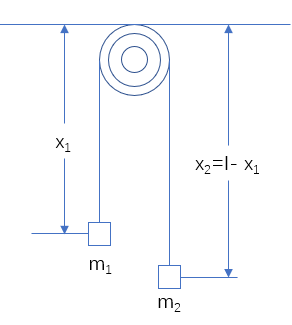
\includegraphics[scale=0.6]{./fig/4-1.png}
    \caption{阿德武德机,包括理想滑轮和二物体}
\end{figure}

\textbf{例}

示于图4-1的体系的质量为$m_1$和$m_2$二质点和无摩擦无重量的滑轮和拉绳,该体系用$F=ma$就能做分析。
但为了说明处理方法,我们用拉格朗日形式来处理。首先,求势能(产生于重力)
\[V=-m_1gx_1-m_2g(l-x_2)\]
式中$l$如图4-1所示。再求动能
\[T=\frac{1}{2}m_1\dot{x}_1^2+\frac{1}{2}m_2\dot{x}_2^2=\frac{1}{2}(m_1+m_2)\dot{x}_1^2\]
因$\dot{x}_1=-\dot{x}_2$。此广义坐标体系是单一坐标$x_1$体系。拉格朗日函数为
\[L=T-V=\frac{1}{2}(m_1+m_2)\dot{x}_1^2+g(m_1-m_2)x_1+m_2gl\]
我们要求算的拉格朗日方程为
\[\frac{\partial L}{\partial x_1}=(m_1-m_2)g\]
\[\frac{\partial L}{\partial \dot{x}_1}=(m_1+m_2)\dot{x}_1\]
因只有一个坐标,故也只有一拉格朗日方程,
\[\dv{t}(m_1+m_2)\dot{x}_1-(m_1-m_2)g=0\]
或
\[(m_1+m_2)\ddot{x}_1=(m_1-m_2)g\]
它与牛顿定律$F=ma$准确地等价。

本章末的习题将说明在牛顿方程比较笨拙的情况下的拉格朗日方程。

做为将牛顿定律表示为拉格朗日方程形式的结果,我们能够导出广义守恒定理:若$\partial L/\partial q_j=0$,则力学量$\partial L/\partial \dot{q_j}$(广义动量)守恒。
若用笛卡儿坐标表示$L$,
\[L=T-V=\frac{m}{2}(\dot{x}^2+\dot{y}^2+\dot{z}^2)-V(x,y,z) \tag{4-32}\]
则$\partial L/\partial x=F_x$,$x$方向的力,$\partial L/\partial \dot{x}=m\dot{x}=p_x$, x方向的动量。
这样,从拉格朗日形式的守恒定理又得出原来的动量守恒定理。我们也可以给出结构平行和权重相同的坐标(或位置)和动量以定义一广义动量。
\begin{definition}[广义动量]
    定义与广义坐标$q_i$共轭的广义动量$p_i$为
    \[p_i=\frac{\partial L}{\partial \dot{q}_i} \tag{4-33}\]
\end{definition}

用此定义,拉格朗日方程能够改写为
\[\dot{p}_i=\frac{\partial L}{\partial q_i} \tag{4-34}\]
用位置和动量来表示力学比单用位置表示其优点有二。
第一,现位置和动量之间的显著的平行结构,它在经典力学和量子力中都构成许多有意义的结果。
第二,可用$6n$个($3n$个$q$和$3n$个$p$)一阶微分方程表示的运动方程代替单用$3n$个($3n$个$q$)二阶微分方程。
即把位置和动量二者都看作是独立变量,这就使我们用两倍的方程式换来了数学上的简化。
为了做到这一点,即用$q's$和$p's$写运动方程,我们先定义一有巨大意义的新力学量。

\begin{definition}[哈密顿函数]
    含几个质点的体系的哈密顿函数为
    \[H=\sum_i p_i \cdot \dot{q}_i-L \tag{4-35}\]
\end{definition}

像前边考虑那样,广义坐标不显含时间,势能与速度无关,我们可以写出
\[\dd{H}=\sum_i\left(\frac{\partial H}{\partial q_i}dq_i+\frac{\partial H}{\partial p_i}dp_i\right) \tag{4-36}\]
由方程4-35得出
\[\frac{\partial H}{\partial q_i}=\sum_ip_i \cdot \frac{\partial \dot{q}_i}{\partial q_i}-\frac{\partial L}{\partial \dot{q}_i}\frac{\partial \dot{q}_i}{\partial q_i}-\frac{\partial L}{\partial q_i} \tag{4-37a}\]
\[\frac{\partial H}{\partial p_i}=\dot{q}_i \tag{4-37b}\]
因$\partial L/\partial \dot{q}_i=p_i$,$\partial L/\partial q_i=\dot{p}_i$,代入方程4-36,得到
\[\dd{H}=\sum_i\left(-\dot{p}_idq_i+\dot{q}_idp_i\right) \tag{4-38}\]
或
\[\dot{q}_i=\frac{\partial H}{\partial p_i} \qquad \dot{p}_i=-\frac{\partial H}{\partial q_i} \tag{4-39}\]
常称方程4-39为哈密顿方程。然而,哈密顿函数的性质是什么?
到目前为止我们只知道一抽象定义,方程4-35。$H$的一重要性质是,它是保守的,或在运动中守恒。
\[\dv{H}{t}=\sum_i\left(\frac{\partial H}{\partial q_i}\dot{q}_i+\frac{\partial H}{\partial p_i}\dot{p}_i\right)+\frac{\partial H}{\partial t}=\sum_i\left(-\dot{p}_i\dot{q}_i+\dot{q}_i\dot{p}_i\right)+\frac{\partial H}{\partial t}=\frac{\partial H}{\partial t} \tag{4-40}\]
从方程可见,除非$H$显函时间,否则$H$与时间无关,或在运动中守恒。
最后,为了将$H$与常见的物理量联系起来,我们集中考察动能:
\[T=\frac{1}{2}\sum_im_iv_i^2=\frac{1}{2}\sum_im_i\left(\sum_j\frac{\partial \mathbf{r}_i}{\partial q_j}\dot{q}_j\right)^2 \tag{4-41}\]
若$\mathbf{r}$不显函时间,则
\[T=\frac{1}{2}\sum_im_i\sum_{jk}\frac{\partial \mathbf{r}_i}{\partial q_j} \cdot \frac{\partial \mathbf{r}_i}{\partial q_k}\dot{q}_j\dot{q}_k=\frac{1}{2}\sum_{jk}t_{jk}\dot{q}_j\dot{q}_k \tag{4-42}\]
式中
\[t_{jk}=\sum_im_i\frac{\partial \mathbf{r}_i}{\partial q_j} \cdot \frac{\partial \mathbf{r}_i}{\partial q_k} \tag{4-43}\]
由此可得
\[\frac{\partial T}{\partial \dot{q}_i}=\sum_kt_{ik}\dot{q}_k \tag{4-44}\]
因而,
\[\sum_i \dot{q}_i\frac{\partial T}{\partial \dot{q}_i}=2T \tag{4-45}\]
现在可援引广义动量的定义,方程4-34。若势能与速度无关则\footnote{原书下式第一个等号后的$L$,写成了$T$(笑}
\[p_i=\frac{\partial L}{\partial \dot{q}_i}=\frac{\partial T}{\partial \dot{q}_i} \tag{4-46}\]
最后,
\[H=\sum_ip_i\dot{q}_i-L=\sum_i\frac{\partial T}{\partial \dot{q}_i}\dot{q}_i-T+V=2T-T+V=T+V \tag{4-47}\]
或,对势能与速度无关的保守系,哈密顿函数是总能量。所有这些结果可用一个定理表示。
\begin{theorem}
对势能与速度无关的保守系,若哈密顿函数不显函时间,则它在运动中守恒,因此在此条件下(总)能量守恒。最后,若$H$不随(广义)坐标变,则与该坐标共轭的动量守恒;若$H$不随动量变,则与该动量共轭的坐标守恒。
\end{theorem}

我们引入最后一个定义做为经典力学中最后一个课题,它与哈密顿处理一起构成联结量子力学和经典力学的途径。
\begin{definition}[泊松括号]
    定义二力学量$F$和$G$的泊松括号为
    \[\{F,G\}=\sum_i\left (\frac{\partial F}{\partial q_i}\frac{\partial G}{\partial p_i}-\frac{\partial F}{\partial p_i}\frac{\partial G}{\partial q_i}\right ) \tag{4-48}\]    
\end{definition}
泊松括号的一个重要应用是它可以示出守恒性质,因
\[\dv{F}{t}=\frac{\partial F}{\partial t}+\sum_i\left(\frac{\partial F}{\partial q_i}\dot{q}_i+\frac{\partial F}{\partial p_i}\dot{p}_i\right)
=\frac{\partial F}{\partial t}+\sum_i\left (\frac{\partial F}{\partial q_i}\frac{\partial H}{\partial p_i}-\frac{\partial F}{\partial p_i}\frac{\partial H}{\partial q_i}\right )=\frac{\partial F}{\partial t}+\{F,H\} \tag{4-49}\]
因此,若$F$不显函时间,则在$F$和$H$的泊松括号为零的条件下$F$在运动中守恒。

在本节中我们介绍了经典力学的两种数学处理。

1.拉格朗日方程。用$3n$个广义坐标表示的$3n$个二阶微分方程:
\[\dv{t}\frac{\partial L}{\partial \dot{q}_i}-\frac{\partial L}{\partial q_i}=0\]

2.哈密顿方程。用$3n$个广义坐标和$3n$个广义动量表示的$6n$个一阶微分方程:
\[\frac{\partial H}{\partial p_i}=\dot{q}_i \qquad -\frac{\partial H}{\partial q_i}=\dot{p}_i\]

这些数学处理能帮助我们记认守恒定理。特别重要的一点是:不显函时间的哈密顿函数在运动中守恒。
在某种常见的情况下,哈密顿函数等于体系的总能量。第五章将示出哈密顿经典力学怎样才能与量子力学联系起来。

\section{力学体系的振动}
在本节中我们将用上节中发展的拉格朗日力学研究质点体系的振动。

$n$个质点的体系有$3n$个自由度;其中有$3$个移动自由度和$3$个转动自由度。
因此,有$3n-6$个振动自由度。对线形分子此简单计算需要修正,线形分子只有$2$个转动自由度,因而振动自由度是$3n-5$。

拉格朗日量是$L=T-V$。因此,需要将$T$和$V$用广义坐标写出。由方程4-42和4-43知
\[T=\frac{1}{2}\sum_{jk}t_{jk}\dot{q}_j\dot{q}_k \tag{4-42}\]
\[t_{jk}=\sum_im_i\frac{\partial \mathbf{r}_i}{\partial q_j} \cdot \frac{\partial \mathbf{r}_i}{\partial q_k} \tag{4-43}\]
$T$是广义速度的二次函数\footnote{原书公式后此句开头有个"或,",感觉句意不通删了。}。$T$还可以用矩阵元为数$t_{jk}$的矩阵表示。

一真实振动分子的势能是一个复杂的和未完全被了解的函数。
但当离开平衡位置的位移很小时,用谐振势能函数作力学体系的振动的简单计算,常常是对真实分子势能的良好近似。
具有这个势能的力学体系称为谐振子;此势能函数与描述服从虎克定律的质点体系的势能函数等同:
\[V=\frac{1}{2}\sum_{jk}v_{jk}q_jq_k \tag{4-50}\]
或,势能$V$是广义坐标的二次函数。$V$也可用其矩阵元为数$v_{jk}$的矩阵表示。

现在可以写出拉格朗日函数
\[L=T-V=\frac{1}{2}\sum_{jk}(t_{jk}\dot{q}_j\dot{q}_k-v_{jk}q_jq_k) \tag{4-51}\]
根据拉格朗日方程,方程4-31,
\[\dv{t}\frac{\partial L}{\partial \dot{q}_j}-\frac{\partial L}{\partial q_j}=0 \tag{4-31}\]
得出
\[\dv{t}\left(\frac{1}{2}\sum_kt_{jk}\dot{q}_k\right)+\frac{1}{2}\sum_kv_{jk}q_k=0\]
\[\sum_k(t_{jk}\ddot{q}_k+v_{jk}q_k)=0 \tag{4-52}\]
不出所料,此方程与简谐运动方程形式上相似;因此,可取尝试解为$q_k=\phi_k\sin\omega t$,$\phi_k$是振幅,$\omega$是振动频率。可得
\[\sum_k\left(v_{jk}\phi_k-\omega^2t_{jk}\phi_k\right)=0 \tag{4-53}\]
这正是变量为$\phi_k$的一组联立线性齐次方程,它有解\footnote{应该是非全零解。}的条件是系数行列式为零:
\[
\begin{vmatrix}
    v_{11}-\omega^2t_{11} & v_{12}-\omega^2t_{12} & \cdots & v_{1n}-\omega^2t_{1n} \\
    v_{21}-\omega^2t_{21} & v_{22}-\omega^2t_{22} & \cdots & v_{2n}-\omega^2t_{2n} \\
    \vdots & \vdots & \ddots & \vdots \\
    v_{n1}-\omega^2t_{n1} & v_{n2}-\omega^2t_{n2} & \cdots & v_{nn}-\omega^2t_{nn}
\end{vmatrix} 
=0 \tag{4-54}   
\]
此方程酷似方程3-82示出的算符的特征值的久期方程。虽然在主对角线上和主对角线以外的特征值都乘以动能矩阵T的矩阵元,但我们也可以将方程4-54叫久期方程。
它有与$\phi_{n'^s}$同样数目的$3n-6$(或$3n-5$)个根$\omega^2$。类似地,可将方程4-53中的方程组写成特征向量方程:
\[V\phi^i=\omega^2T\phi^i \tag{4-55}\]
即,$V$作用于$\phi^i$给出$T$作用于$\phi^i$的倍数($\omega_i^2$)。
\begin{theorem}
    特征值$\{\omega^2\}$必须是非负的和实的。
\end{theorem}

此定理可沿上一章给出的相同的路线加以证明。$\omega^2$是非负的就已充分了,因这样$\omega$必是实的。我们可用另一形式的定理回答分子振动的特征值问题。
\begin{theorem}
特征向量$\{\phi^i\}$形成的以$\{\phi^i\}$为列的矩阵$\Phi$通过下列变换可同时将$V$和$T$对角化:
\[\Phi'V\Phi=\Omega \tag{4-56a}\]
\[\Phi'T\Phi=E \tag{4-56a}\]
式中$\Omega$是其对角元为$\omega^2$的可能值的矩阵,E是单位矩阵。
\end{theorem}

这里的变换虽具有$\Phi'V\Phi$和$\Phi'T\Phi$的形式,但不是相相似变换。方程中的变换称为迭合变换\footnote{特征向量集是相互正交的,转置等于逆,所以这里说是相似变换也没问题。}。用矩阵$\Omega$和$\Phi$可将特征值方科4-55改写成
\[V\Phi=T\Phi\Omega \tag{4-57}\]
左乘$\Phi'$,得
\[\Phi'V\Phi=\Phi'T\Phi\Omega \tag{4-58}\]
将它与习用的特征值问题(如方程3-86)的对应结果比较。因$\Phi'$是正交的,故方程3-86可改写为
\[\Phi'Q\Phi=\Phi'\Phi\hat{q} \tag{3-86}\]
在方程4-58中,方程3-86的$\Phi'\Phi$被$\Phi'T\Phi$替代;这可与方程4-54和方程3-82之间的差别比较。
事实上,正如方程3-86中$\Phi'\Phi=E$(单位矩阵)那样,我们可以证明方程4-58中$\Phi'T\Phi$也是单位矩阵。
因为$\phi^j$对方程4-55的左乘内积为
\[\bra*{\phi^j}V\ket*{\phi^i}=\omega_i^2\bra*{\phi^j}T\ket*{\phi^i} \tag{4-59}\]
$\phi^j$右乘的内积为
\[\bra*{V\phi^i}\ket*{\phi^j}=\omega^2_j\bra*{T\phi^i}\ket*{\phi^j}\]
\[\bra*{\phi^j}\ket*{V\phi^i}=\omega^2_j\bra*{\phi^j}T\ket*{\phi^i} \tag{4-60}\]
故比较方程4-59和4-60,可得
\[(\omega_j^2-\omega_i^2)\bra*{\phi^j}T\ket*{\phi^i}=0 \tag{4-61}\]
或,因特征值不同$\omega_j^2 \neq \omega_i^2$,故$\bra*{\phi^j}T\ket*{\phi^i}=0$。最后,对向量$\{\phi^i\}$作适当地调整,我们可以得出对所有$\phi^j$ ,$\bra*{\phi^j}T\ket*{\phi^j}=1$。
这些陈述和在通常的特征值问题中特征向量的正交归一性类似。

因此,可以得出如方程4-56b那样,中$\Phi'T\Phi=E$,如方程4-56a那样,方程4-58变成$\Phi'V\Phi=\Omega$。

用一个说明如何将这种处理方法应用于分子振动的简单例子结束这一节。
应该在开始时就指出,比这里介绍的方法更复杂的方法也可以用,并且也已被用于复杂分子的振动。
但问题的一般特点及其解法是相同的。

\textbf{例}

有一分子只沿直线振动(这是实际不存在的简化)。如图4-2所示分子是对称的。
我们需要先求算在示出的坐标系(这只是做为例子——也可以选其它坐标系)中势能和动能,然后将势能和动能表示为矩阵。
先考虑势能。在作谐振子近似中势能用一些项表示,每一项是键扩张的平方乘虎克定律力常数:
\[V=\frac{k}{2}(x_2-x_1-b)^2+\frac{k}{2}(x_3-x_2-b)^2\]

\begin{figure}[htbp]
    \centering
    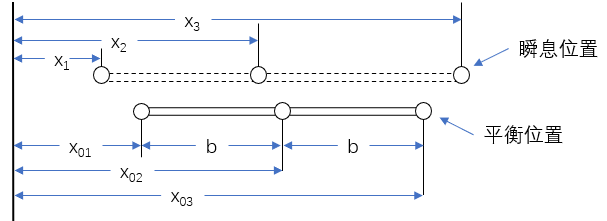
\includegraphics[scale=0.5]{./fig/4-2.png}
    \caption{描述线形三原子分子的坐标系}
\end{figure}

我们需要将势能写为位移坐标\footnote{作者没有在开始指明三个小球的质量,两端的小球质量为m,中间的小球质量为M。}。定义最左边质点的平衡位置为$x_{01}$,中心质点的平衡位置为$x_{02}$,最右边质点的平衡位置为$x_{03}$。
然后,定义位移坐标如下:
\[ 
\begin{array}{c}
    q_1=x_1-x_{01} \\
    q_2=x_2-x_{01} \\
    q_3=x_3-x_{01}
\end{array}
\]
因
\[b=x_{02}-x_{01}=x_{03}-x_{02}\]
故
\[V=\frac{k}{2}(q_2-q_1)^2+\frac{k}{2}(q_3-q_2)^2=\frac{k}{2}(q_1^2+2q_2^2+q_3^2-2q_1q_2-2q_2q_3)\]
现在我们可以写出势能的矩阵。矩阵元$v_{ij}$是势能表示式中项$q_iq_j$的系数。这意味着势能矩阵是
\[V=
\begin{pmatrix}
    k & -k & 0 \\
    -k & 2k & -k \\
    0 & -k & k
\end{pmatrix}
\]
动能比较简单些。在图4-2示出的坐标系中动能是
\[T=\frac{m}{2}(\dot{x}_1^2+\dot{x}_3^2)+\frac{M}{2}(\dot{x}_2^2)\]
若将位移坐标和它的时间导数代入此方程,可得
\[T=\frac{m}{2}(\dot{q}_1^2+\dot{q}_3^2)+\frac{M}{2}(\dot{q}_2^2)\]
也取$T$中的各项(此情况下只有三项),并放到矩阵中去,矩阵中的$t_{ij}$是$T$中$q_iq_j$的系数,可得出动能矩阵
\[T=
\begin{pmatrix}
    m & 0 & 0 \\
    0 & M & 0 \\
    0 & 0 & m
\end{pmatrix}
\]
特征值方程为
\[V\Phi=\omega^2T\Phi\]
需解的久期方程是
\[|V-\omega^2T|=0=
\begin{vmatrix}
    k-\omega^2m & -k & 0 \\
    -k & 2k-\omega^2M & -k \\
    0 & -k & k-\omega^2m
\end{vmatrix}
\]
用行的余因式很容易将久期行列式展开\footnote{这里对运算过程和结果的表示方法做了省略,不影响作者想表达的意思。}:
\[0=(k-\omega^2m)
\begin{vmatrix}
    2k-\omega^2M & -k \\
    -k & k-\omega^2m
\end{vmatrix}
+k
\begin{vmatrix}
    -k & -k \\
    0 & k-\omega^2m
\end{vmatrix}
=(k-\omega^2m)(\omega^2)[\omega^2Mm-k(M+2m)]
\]
其解为
\[\omega=\sqrt{\frac{k}{m}} \ ,\ 0 \ , \ \sqrt{\left(\frac{k}{m}\right)\left(1+\frac{2m}{M}\right)}\]

根据已发展的理论,特征值存在零解不被禁阻。我们只发现特征值$\omega^2$不能是负值。
如果读者返回去并考察理论在那个问题上的发展,他就可得出如下的结论,特征值$\omega=0$对应于其自由度的势能为零的某种运动。
具有零势能的体系并不是谐振子;它是无恢复力或反向力的某种运动。换句话说,它表示自由移动或自由转动。

这也是我们应该预期到的一点。前边我们用三个广义坐标描述此问题,但只应有两个坐标。
我们没有消去对应于与$x$轴平行的移动的广义坐标。这说明了一个重要问题,
非振动的分子运动若仍保留在被选取的广义坐标系中,则它的特征值$\omega^2$为零。

使用一组与振动联系着的只含二坐标的坐标系,我们能重新处理此问题。
为此,应写出我们希望禁阻的移动的方程,并用它来消除以前用的三个坐标$q_1,q_2,q_3$中的一个。
能够选取此方程的条件是使体系的质心在原点:
\[m(x_1+x_3)+Mx_2=0\]
进一步作下去可得到同样的非零特征值,但没有零特征值。

现在我们面临的问题是求简正振动的特征向量。为此,须将特征值(现为已知量)代回到特征值特征向量方程,解此方程求特征向量的分量。
每一特征值就有一特征向量,因此有几个特征值,此过程就要进行几\footnote{此处原文为“n”,与上文对不上,故改为"几"。}次。
振动问题和通常的特征向量问题不同,它不要求特征向量归一化为一,而要求$\bra*{\phi^i}T\ket*{\phi^i}=1$。
特征值方程为$V\Phi=\omega^2T\Phi$。第-次计算选取特征值$\omega^2=k/m$,得到
\[
\begin{pmatrix}
    k & -k & 0 \\
    -k & 2k & -k \\
    0 & -k & k
\end{pmatrix}    
\begin{pmatrix}
    \phi^1_1 \\ \phi^1_2 \\ \phi^1_3
\end{pmatrix}
=\frac{k}{m}
\begin{pmatrix}
    m & 0 & 0 \\
    0 & M & 0 \\
    0 & 0 & m
\end{pmatrix} 
\begin{pmatrix}
    \phi^1_1 \\ \phi^1_2 \\ \phi^1_3
\end{pmatrix}  
\]
将矩阵方程写成联立线性方程组
\[k\phi_1^1-k\phi_2^1=k\phi_1^1\]
\[-k\phi_1^1+2k\phi_2^1-k\phi_3^1=\frac{kM}{m}\phi^1_2\]
\[-k\phi_2^1+k\phi_3^1=k\phi_3^1\]
从第一个方程和最后一个方程得到
\[\phi^1_2=0\]
代入第二个方程得到
\[\phi_1^1=\phi_3^1\]
一个可接受的特征向量(在归一化以前) 是向$(a,0,-a)$。
需要与归一化类似的处理,$\bra*{\phi^i}T\ket*{\phi^i}=1$。以矩阵形式表示为:
\[
(a \ , \ 0 \ , \ -a) 
\begin{pmatrix}
    m & 0 & 0 \\
    0 & M & 0 \\
    0 & 0 & m
\end{pmatrix}
\begin{pmatrix}
    a \\ 0 \\ -a
\end{pmatrix}  
=  
\begin{pmatrix}
    a & 0 & -a
\end{pmatrix} 
\begin{pmatrix}
    ma \\ 0 \\ -ma
\end{pmatrix}  
=2a^2m=1
\]
所以,$a=1/\sqrt{2m}$。因此,归一化的特征向量为$(1/\sqrt{2m},0,-1/\sqrt{2m}$。

对特征值$\omega^2=(k/m)(1+2m/M)$,用同样过程给出未归一化的特征向量为$(a,-2ma/M,a)$
归一化的特征向量十分复杂,为
\[\left(\sqrt{\frac{M}{2mM+4m^2}},-\sqrt{\frac{4m}{4mM+2M^2}},\sqrt{\frac{M}{2mM+4m^2}}\right)\]
特征值$\omega^2=0$的特征向量也可以计算,未归一化的特征向量为$(a,a,a)$;归一化的特征向量的每个分量为$1/\sqrt{2m+M}$。

做为对振动问题的解的最后验证,我们对非对角型的$V$矩阵和对$T$矩阵实施变换。
结果应给出,$V$矩阵变换成以特征值$\omega^2$为对角元的对角矩阵,$T$矩阵变换为单位矩阵。

为简便计,考虑三原子线形分子,如$N_3^-$或$I_3^-$,因而$m=M$。
特征向量为
\[\left(\sqrt{\frac{1}{2m}},0,-\sqrt{\frac{1}{2m}}\right) \ , \ 
\left(\sqrt{\frac{1}{6m}},-\sqrt{\frac{2}{3m}},\sqrt{\frac{1}{6m}}\right) \ , \ 
\left(\sqrt{\frac{1}{3m}},\sqrt{3m},-\sqrt{\frac{1}{3m}}\right)\]
可用图解法解释这些特征向量。特征向量$(1/\sqrt{2m},0,-1/\sqrt{2m})$表示当最左边的原子向左移动时,最右边的原子向右移动,或相反。
这叫做振动的对称伸长方式,示于图4-3a。另一方面,特征向量$(1/\sqrt{6m},-2/\sqrt{6m},1/\sqrt{6m})$表示端原子(1和3)朝同方向运动,而中心原子(2)朝相反方向运动。
中心原子移动的距离为端原子移动距就的二倍以保持质心不变。这叫做反对称伸长方式,示于图4-3b。

最后一个特征向量$(1/\sqrt{3m},\sqrt{3m},-1/\sqrt{3m})$不保持质心固定。事实上此特征向量对应于分子的匀速移动。这是对应于特征频率为零的特征向量。

\begin{figure}[htbp]
    \centering
    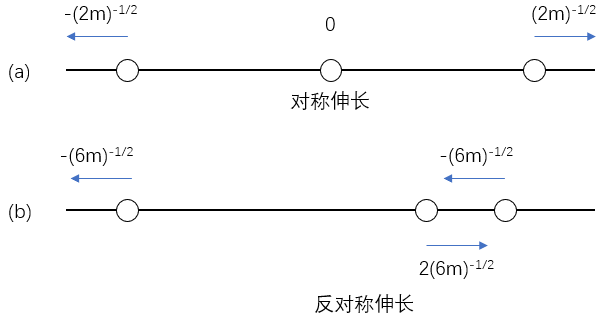
\includegraphics[scale=0.5]{./fig/4-3.png}
    \caption{线形三原子分子的振动的简正方式}
\end{figure}

\section{刚性力学体系的转动}
在上节中我们发展了振动力学体系的运动方程,并证明那种分析如何用到分子振动。
在本节中要发展转动力学体系的运动方程,并要证明如何应用于分子转动。
如上节末指出那样,有比这里介绍的方法更优异的方法可用;下边的讨论只是对一般问题作一概述。

对力学体系可求拉格朗日方程(方程4-31)的解,方程中的拉格朗日函数是按方程4-30定义。
对$V=0$因而$L=T$的刚性体系\footnote{刚性分子骨架的假定自然是不正确的,因分子确在振动,然而此假定可使讨论简化,并能使一些有兴味的概念显现出来。同样地,对阻尼转动这一非常有兴味的情况假定$V=0$也是不正确的。}
的转动拉格朗日函数特别简单。

刚性转动的动能的形式也特别简单。因为按定义
\[T=\frac{1}{2}\sum_im_iv_i^2 \tag{4-62}\]
故需对转动的$v_i$加以说明。简单的图可使同学们确信,对于圆周运动
\[\mathbf{v}_i=\omega \times \mathbf{r}_i \tag{4-63}\]
式中$\omega$是角速度。在一般情况下方程4-63成立。应用方程4-63,则方程4-62变为
\[T=\frac{1}{2}\sum_im_i\mathbf{v}_i \cdot (\omega \times \mathbf{r}_i) \tag{4-64}\]
可以证明方程4-64的乘积中的向量的顺序可以改变,给出
\[T=\frac{\omega}{2}\sum_im_i(\mathbf{r}_i \times \mathbf{v}_i)=\frac{\omega}{2}\sum_i\mathbf{l}_i=\frac{1}{2}\omega \cdot \mathbf{L} \tag{4-65}\]
式中$\mathbf{l}_i$是第$i$个质点的角动量,$\mathbf{L}$是整个体系的角动量。

而
\[\mathbf{L}=\sum_im_i(\mathbf{r}_i \times \mathbf{v}_i)=\sum_im_i(\mathbf{r}_i \times (\omega \times \mathbf{r}_i))=\sum_im_i(\omega\mathbf{r}_i^2-\mathbf{r}_i(\mathbf{r}_i-\omega)) \tag{4-66}\]
使用转动惯量张量的定义可将方程4-65改写成简缩的形式。
\begin{definition}[转动惯量张量]
    绕某一点转动的物体的转动惯量张量是一对称矩阵,在笛卡儿坐标系里定义如下。
    令$q_1^v,q_2^v,q_3^v$号为质点的$x,y,z$坐标。转动惯量的$i,j$元定义为:
    \[I_{ij}=\sum_pm_p(\mathbf{r}_p^2\delta_{ij}-q_i^vq_j^v) \tag{4-67}\]
    式中$\mathbf{r}_p$是质点$P$与特定点的距离。
\end{definition}

用$I$的这个定义可写出
\[\mathbf{L}=\mathbf{I}\omega \tag{4-68}\]
因此
\[T=\frac{1}{2}\omega \cdot \mathbf{I}\omega=\frac{1}{2}\bra*{\omega}\mathbf{I}\ket*{\omega} \tag{4-69}\]
现在摆在我们面前的问题是怎样精确地解释转动动能公式中的转动惯量张量的作用。

在4-1节中我们学过质点体系绕点转动的角动量,可分解为各质点绕质心转动的角动量加质心的角动量。
因此,如果我们只将注意力集中在分子的转动上,即如果我们为分子取的坐标系是使质心固定不动,则角动量就是绕质心转动的角动量。
于是方程4-67中的$\mathbf{r}_p$可取为质心到质点$p$的距离。

若选的坐标系可能使$\mathbf{I}$是对角的,如为$\xi,\eta,\varsigma$坐标系,则动能可取特别简单的形式
\[T=\frac{\omega \cdot \mathbf{I}\omega}{2}=\frac{1}{2}\left(\mathbf{I}_{\xi\xi}\omega_{\xi}^2+\mathbf{I}_{\eta\eta}\omega_{\eta}^2+\mathbf{I}_{\varsigma\varsigma}\omega_{\varsigma}^2\right) \tag{4-70}\]
式中$\mathbf{I}_{\xi\xi},\mathbf{I}_{\eta\eta},\mathbf{I}_{\varsigma\varsigma}$是$\mathbf{I}$的三个对角元,
$\omega_{\xi},\omega_{\eta},\omega_{\varsigma}$是角速度向量的分量。

$\mathbf{I}$能对角化吗?能,因为$\mathbf{I}$是对称的和实的。当$i \neq j$时,
\[\mathbf{I}_{ji}=\sum_p(-m_pq_i^pq_j^p)=\sum_p(-m_pq_j^pq_i^p)=\mathbf{I}_{ji} \tag{4-71}\]
因$\mathbf{I}$是厄米矩阵,故可求助于3-4节中有关厄米算符的特征值的定理。
因此,称为主转动惯量的$\mathbf{I}$的特征值是实的,称为主轴的特征向量是正交归一的。
联系任意笛卡儿轴系和主轴系的相似变换称为主轴变换。如将$\mathbf{I}$的矩阵对角化,我们马上就可使用$T$的更简单的表示式(方程4-70)来讨论刚性转子的能量。

对刚性转子,习惯上是按等价主转动惯量的数目命名如下
\footnote{为方便打表对原书下表稍作修改。}:
\[
\begin{tabular}{c|c}
    \hline
    等价转动惯量数量 & 转子名称 \\ \hline
    3 & 球陀螺 \\
    2 & 对称陀螺 \\
    none & 非对称陀螺 \\
    \hline
\end{tabular}
\]

\textbf{例}

计算水的主转动惯量。若水分子的取向如图4-4示出的坐标系中那样,则容易算出在此坐标系中转动惯量张量质心在原点的矩阵元。
应注意,分子的取向对称于位于坐标系原点的质心。我们必须先计算可给出分子图4-4水分子的主轴的几何形状的核的位置。
因为质心在原点,故此计算可用简单的三角学和质心的方程
\[\sum_im_i\mathbf{r}_i=0\]
核的位置是\footnote{书上氢原子的坐标还少了负号(emmm}
$\mathbf{r}(0)=(0.00,0.07),\mathbf{r}(H_a)=(-0.76,-0.55),\mathbf{r}(H_a)=(0.76,-0.55)$:
$|\mathbf{r}(0)|=0.07,|\mathbf{r}(H_a)|=|\mathbf{r}(H_b)|=0.94$。
应用方程4-67,可计算出水绕质心转动的转动惯量张量。例如,
\[\mathbf{I}_{xx}=\sum_pm_p(\mathbf{r}^2_p-x_p^2)=[16(0.0049-0.0000)+1(0.881-0.578)+1(0.881-0.578)](M)(10^{-16})\]
\[=1.21 \times 10^{-40}g \cdot cm^2\]
式中M是质子的质量$1.67 \times 10^{-24}g,1\AA^2=10^{-16}cm^2$。同样地
\[\mathbf{I}_{xy}=-\sum_pm_px_py_p=-[(16)(0)(0.07)-(1)(-0.76)(-0.55)-(1)(0.76)(-0.55)](M)(10^{-16})=0\]
用类似的办法可计算出张量$\mathbf{I}$
\[\mathbf{I}=
\begin{pmatrix}
    1.21 \times 10^{-40} & 0 & 0 \\
    0 & 1.93 \times 10^{-40} & 0 \\
    0 & 0 & 3.08 \times 10^{-40}
\end{pmatrix}
\]
因张量是对角化的矩阵,故立刻就可求出主转动惯量。我们还可求出,图4-4上的$x,y,z$轴是主轴。
\begin{figure}[htbp]
    \centering
    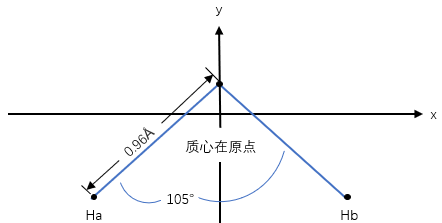
\includegraphics[scale=0.5]{./fig/4-4.png}
    \caption{水分子的主轴}
\end{figure}

这种分子分类和用矩阵代数求主转动惯量的方法在前一节中已发挥了促进作用。

\begin{problemset}
\item 证明方程4-3下边所讲的有关叉乘的性质。
\item 证明在4-1节中提出的质点系的三个守恒定理。
\item 证明在4-1节中提出的三个分离定理。
\item 用一刚性、无重、长度为$l$的棒将质量为$m$的二质点联结起来;棒的中心在用金属丝围成的半径为$a$的圆环上作无摩擦的运动。选用适合的简单的广义坐标组,并用此坐标组将$T$表示出来。
\item 写出在三维空间运动的摆的拉格朗日方程;用刚性的、无重的榜悬挂的质量为$m$的质点在重力的作用下运动。
\item 用一弦(无重、非弹性)将质量不等的二质点联结起来。一质点放在桌子上,另一质点放在桌子一边滑动(无摩擦)。用拉格朗日力学描述此运动。
\item 由弹簧将一质量为$m$的球联于平滑台的中心。弹簧的力常数为$k$,平衡长度为$r$。求体系的运动方程,并加说明。
\item  (a)推导方程4-23a;(b)推导方程4-23b。
\item 一质点在矩形箱内由四个弹簧拉住,每两个弹簧的力常数相同。让质点离开平衡位置一小的位移。描述其运动。
\item 推导方程4-53。
\item 重新推导4-3节的例中提示的用质心坐标系表示的线形三原子分子的简正方式的公式。
\item 求水分子振动的简正方式和频率。
\item 求二氧化碳分子振动的简正方式和频率。
\item 推导方程4-63,4-65和4-66。
\item 证明欧拉定理:有一点固定的刚体的最一般的位 移是绕其轴转动。
\item 计算4-4节的例中水的转动惯量张量,但取另一坐标系;氧原子在原点,-O-H键在$x$轴上。将计算结果和例中的结果比较。
\item 分子$CCl_4, NCl_3,OCl_2,FCl$都是第二周期元素的氯化物。计算每一分子的主转动惯量,并按“陀螺”的特殊种类分类,对每个分子划出简图,并示出其主轴。应查阅这些分子的结构。
\item 证明正四面体和立方体分子是“球顶”。
\end{problemset}
\chapter{总结}
本书的前四章是为量子力学,特别是为分子光谱学准备舞台而设计的。
为了完成舞台道具的准备(事实上是将幕稍启)我们要触及两点。
第一,经典力学和量子力学之间的联系,第二,波动力学观点和矩阵力学观点的综合。

\section{经典力学和量子力学之间的桥}
欲严格地介绍量子力学,应该先知道在十九世纪末和二十世纪初那些令人激动的实验,这些实验要求的理论说明,不是来自牛顿力学和麦克斯威电磁学。
重温此背景将使我们离开本书的目的。因此,本节限定在基本理论的水平上比较经典力学和量子力学,至于量子力学的实验基础则留给读者到别处去欣赏。

按传统的讲法,量子力学课是从评述经典力学的失败开始。对量子力学的最常用的处理方法,是用波动-微粒二象性这个十分自然的观点,并以德布罗意的工作为例。
在开始时就应该认识到,习惯上将经典波动方程和德布罗意的动量波长关系式结合,并不是薛定谔方程的推导,而薛定谔方程则是量子力学发展的基本方程。
只能将薛定谔方程做为假定,从这个假定出发形成对物理世界的看法。此看法只借助相对论和场论的导引在描述亚微观物质上取得巨大的成就。无论如何,波动力学不能推导而只是假定。
量子力学的另一种处理方法,更抽象和更基本些,是建立算符和对应的力学量之间的联系。沿此方向就能提出量子力学的简单的和自洽的一组假定,这些假定是抽象的和基本的。
再一次提出,在开始时就不应把这里讲的处理方法理解为推导,只能理解为假定。它比薛定谔力学的物理内容既不多也不少。作者希望, 用第三章和第四章的术语陈述量子力学而不用人们可能不太熟悉的波动术语,
至少在比较量子力学和经典力学时,会产生新的认识,甚至可能使在两种物理学之间的峡沟上搭桥,不是信念的飞跃而是推理的发展。

玻尔认为,由于经典力学对宏观体系是“正确的”,因此量子力学的引入不能全盘根除过去的经典理论。量子力学必须把经典力学做为极限情况包括在内。
这种陈述木身可以看做是对应原理。怎样用公式表示出由量子力学得到经典力学的极限的本性呢?这个问题能在许多复杂的水平上回答。
这里只给一种指出量子力学的经典极限的方法以及它们之间的对应性;还有别的表示这种对应性的方法。

例如,按$Dicke$和$Wittke$的处理,我们可从量子力学的下述假定开始:每个物理可测量结果是对应该量的算符的本征值。

在经典力学极限中,物理量的算符特性失去了;或更精确讲,物理量$Q$的算符$\mathscr{Q}$必须用“$Q$乘被作用函数”来定义,即$\mathscr{Q}f \rightarrow Qf$。
若这一点成立,那么在经典力学极限中对应于物理的全部算符是可对易的。在唯有量子力学才能“正确地”描述问题的情况下,全部算符是不可对易的。因此, 量子力学的经典力学极限的本性必定是
\[[\mathscr{A},\mathscr{B}]=\text{(小的数)(对应于A,B的某函数的算符)} \tag{5-1}\]
在发展最子理论的过程中,一个“小的数”一次又一次地出现。这个数是普朗克常数。事实上,方程5-1中的数就是$\hbar$这在理论最终与实验比较中得到证实。现在
\[[\mathscr{A},\mathscr{B}]=i\hbar\text{(对应于A,B的某函数的算符)} \tag{5-2}\]
我们对经典力学和量子力学之间的对应性的寻找,差不多完成了。由于量纲的原因,“A,B的函数”的量纲,必须是($AB$/尔格-秒)因为$i\hbar$的单位是尔格-秒。这样的函数就是$A$和$B$的泊松括号因此,
\[[\mathscr{A},\mathscr{B}]=i\hbar\text{(对应于$\{A,B\}$的算符)} \tag{5-3}\]
它就是$Dicke$和$Wittke$的第七个假定。方程5-3不是推导出来的,而是“规定”或“辅助导引”出来的。
从经典力学和量子力学之间的对应性和极限的陈述出发,我们可以推导(现在用推导这个词是正确的)出一些重要的结果。

第一,比较力学量和哈密顿函数的泊松括号,与对应的算符和哈密顿算符的换位子。
\[\dv{f}{t}=\{f,H\}+\frac{\partial f}{\partial t} \tag{4-48}\]
再求助于经典力学极限的原理,算符$\mathscr{F}$的行为就像函数$f$一样,
\[\dv{\mathscr{F}}{t}=-\frac{i}{\hbar}[\mathscr{F},\mathscr{H}]+\frac{\partial \mathscr{F}}{\partial t}=\frac{i}{\hbar}[\mathscr{H},\mathscr{F}]+\frac{\partial \mathscr{F}}{\partial t} \tag{5-4}\]
这就是海森堡运动方程。海森堡的观点(重点放在线性算符及其矩阵表示),将力学量的全部时间变量通过方程5-4放到其对应的算符中。
此方程使我们能用守恒定理来表述对应原理:在经典力学中运动守恒的量,在量子力学中仍然是运动守恒的量。
例子\footnote{原文为“特例”,我觉得是翻译的问题,原作者可能想表达强调。}是,若经典哈密顿量不显函时间,则能量是守恒的:
\[\dv{H}{t}=\{H,H\}+\frac{\partial H}{\partial t}=\{H,H\}=0 \tag{5-4a}\]
其量子力学的类似关系为
\[\dv{\mathscr{H}}{t}=\frac{i}{\hbar}[\mathscr{H},\mathscr{H}]+\frac{\partial \mathscr{H}}{\partial t}=\frac{i}{\hbar}[\mathscr{H},\mathscr{H}]=0 \tag{5-4b}\]

薛定谔用的另一种观点
\footnote{原书的脚注:这里使用“观点”一词表示运动方程在量子力学中是用什么方式来描述,别的作者用“表示”表示此概念如“海森堡表示”薛定得表示”。但我们用“表示”表示十分不同的意思,因而这里不用它。}
,是使算符不显函时间,而其本征值显函时间。为此,开始时用其本征函数为$\phi$的算符的本征值$f$的运动方程。
\[\dv{\mathscr{F}}{t}=\dv{t}\bra*{\phi}\mathscr{F}\ket*{\phi}=\bra*{\dv{\phi}{t}}\mathscr{F}\ket*{\phi}+\bra*{\phi}\mathscr{F}\ket*{\dv{\phi}{t}} \tag{5-6}\]
由方程5-4得
\[\dv{\mathscr{F}}{t}=\bra*{\phi}\frac{i}{\hbar}[\mathscr{H},\mathscr{F}]\ket*{\phi}=\bra*{\phi}\frac{i}{\hbar}\mathscr{H}\mathscr{F}-\frac{i}{\hbar}\mathscr{F}\mathscr{H}\ket*{\phi}\]
\[=\bra*{-\frac{i}{\hbar}\mathscr{H}\phi}\mathscr{F}\ket*{\phi}+\bra*{\phi}\mathscr{F}\ket*{-\frac{i}{\hbar}\mathscr{H}\phi} \tag{5-7}\]
为使方程5-6和方程5-7一致,则要求
\[\mathscr{H}\phi=i\hbar\frac{\partial \phi}{\partial t} \tag{5-8}\]
这就是薛定谔方程。

这样,我们就看到了经典力学和量子力学之间的简洁的对应关系能够建立起来,它既可引出海森堡运动方程又能引出薛定谔运动方程,并伴随着守恒定理。

\section{矩阵力学和波动力学的综合}
我们已经讲了本征值-本征向量问题的两种观点。在第一种观点里,算符是微分算符,因而本征值方程是微分方程。
在第二种观点里,算符用矩阵表示,因而本征值方程是用一组联立线性齐次方程表示。这两种观点的综合可在希伯特空间的概念中找到。

我们需要证明,第三章的代数法仍可应用于连续变量问题(许多量子力学问题所具有的)。
若定义希伯特空间为,由有定义内积(方程3-1)的归一化函数张成的向量空间,那我们就可以建立矩阵力学和波动力学的综合。
希伯特空间的概念允许向量空间是无限维的。此无限个数可以是分立的,并且可如基组$\{H_n(x)\}$中指标$n$那样标记为$n=0,1,2\cdots$。或此无限个数可以是连续的,如直线上的点那样不能用数标记。

对希伯特空间作进一步讨论使我们离题太远;作者只希望指出特征函教和特征向量之间的相似性质。
在希伯特空间里,算符的相阵表示可以是无限维的;本征函数可用无限长的列向量表示。
例如,位置算符$\mathscr{X}$具有连续域,或特征值谱,如$\{x'\}:\mathscr{X}\ket*{x'}=x'\ket*{x'}$。
希伯特空间中的任何本征向量$\ket*{\xi'}$都可用$\mathscr{X}$的本征向量(因为它们形成一完备正交归一组)展开。
\[\ket*{\xi}=\sum\ket*{x'}\bra*{x'}\ket*{\xi}=\int\ket*{x'}\bra*{x'}\ket*{\xi}\dd{x} \tag{5-9}\]
因希伯特空间是无限维的,所以我们用对连续变量$x'$积分代替求和。系数$\bra*{x'}\ket*{\xi}$是(复)函数,它组成以$\ket*{x'}$为基的向量$\ket*{\xi}$的表示。
我们可称此复函数集合为波函数:$\Psi_{\xi}(x')=\bra*{x'}\ket*{\xi}$。二希伯特空间向量的内积$\bra*{\xi}\ket*{\eta}$给出与第二章的理论的最终联系:
\[\bra*{\xi}\ket*{\eta}=\int \dd{x}'\int \dd{x}''\bra*{\xi}\ket*{x'}\bra*{x'}\ket*{x''}\bra*{x''}\ket*{\eta}=\int \dd{x}'\bra*{\xi}\ket*{x'}\bra*{x'}\ket*{\eta}=\int \dd{x}'\Psi_{\xi}^*(x')\Psi_{\eta}(x') \tag{5-10}\]
它与方程2-1相同\footnote{原文5-10式最后一个等号后面的$\Psi_{\eta}(x')$误写为$\Psi^*_{\eta}(x')$(笑}。

到此,我们结束了对与量子化学有关的数学和物理的突击。作者的希望,是同学们在量子力学的原理和应用的过程中,不要被同时紧张地领会表达量子力学的数学语言所羁绊。

\begin{problemset}
\item 证明方程5-3的量纲是正确的。
\item 应用方程5-3所表达的对应原理,求笛卡儿坐标和笛卡儿直线动量之间的对易关系。
\end{problemset}
\end{document}
